\chapter{Rio de Janeiro Mangroves} \label{ch:mangroves}

\section{\hlc[cyan]{Chapter Purpose \& Structure}}

The case study detailed in this chapter is in service to multiple objectives. First, it seeks to address Research Question 2: ``What are the sustainability benefits of collaborative development of \acp{dss} using the \acf{evdt} Modeling Framework in complex \acf{sets}?" It accomplishes this by providing a case study demonstration of Research Deliverables 2a, 2b, and 2c: 

\begin{enumerate}[label=\emph{\alph*},itemsep=0pt,parsep=0pt]
	\item{System architecture analyses of each of the case studies} 
	\item{Development of an \ac{evdt}-based \acf{dss} for each of the case studies} 
	\item{An interview-based assessment of the development process and usefulness of each \ac{dss}} 
\end{enumerate}
	
Through these deliverables, this chapter serves as a demonstration of the \ac{evdt} Framework. The structure of this chapter thus mirrors the components of the framework laid out in Section \ref{sec:framework}. It starts by walking through the steps of the \acf{saf} as applied to this case study in Section \ref{sec:rio-saf}. These are separated into the methodology used for each step of the \ac{saf} (Section \ref{sec:rio-saf-method}) and the results of each step (Section \ref{sec:rio-saf-results}. Then, in Section \ref{sec:rio-evdt}, it shall turn to showing relevant datasets and analysis as applied through the \acf{evdt} models. These two are separated in methodology (Section \ref{sec:rio-evdt-method}) and results (Section \ref{sec:rio-evdt-result}. These are then integrated into a prototype \ac{dss} in Section \ref{sec:rio-dss}. Finally Section \ref{sec:rio-collab} lays out how various stakeholders were collaborated with beyond the setting of requirements during the \ac{saf} process. The remaining sections examine and discuss the outcomes of this case study. The following chapter will similarly present a second case study.  

It should be noted that, as stated in Section \ref{sec:questions}, each case study also has its own objectives beyond supporting a chapter of this thesis. In this case, that means supporting policy decisions in Rio de Janeiro surrounding human wellbeing and mangrove conservation. Readers specifically interested in the socio-environmental history of the study area are pointed to Section \ref{sec:rio-context}. Those interested in environmental analyses performed in the course of this research are pointed to Sections \ref{sec:rio-evdt-e-method}, \ref{sec:rio-evdt-e-result}, and \ref{sec:rio-discussion}.

Finally, this research was begun in 2017. Field visits took place in 2019 and 2020, the latter of which was interrupted by the onset of the COVID-19 pandemic (as was this project in general). Our research and development priorities (both mine and those of our Rio de Janeiro colleagues) shifted to more urgent concerns. This means that aspects of this chapter are a couple of years old at the time of writing and various desired objectives were never reached. This is discussed further in Section \ref{sec:rio-discussion}.

\section{\hlc[cyan]{A Note on Credit / Contributions}}

Prior to this project, I had little experience with mangroves and no experience with Brazil. This project would not have been possible without the contributions of quite a number of people, some of whom I would like to acknowledge here.

\begin{itemize}[itemsep=0pt,parsep=0pt]
	\item{Felipe Mandarino: Served as my primary point-of-contact over the course of several years and was the anchor of this project.}
	\item{David Lagomasino: Taught me how to use \ac{gee} and work with satellite imagery.}
	\item{Carla Madureira, Rafael Silva de Barros, and all of their students at \ac{ufrj}: Taught me about the local mangroves, took me on field visits, and helped me to buy my first pair of Havaianas.}
	\item{Suhyun Jung and Emily Joiner: Taught me about ecosystem services and compiled many of the valuation studies referred to in this chapter.}
\end{itemize}


\section{\hlc[green]{Systems Architecture Framework}} \label{sec:rio-saf}

The following subsections work through the six steps of the \ac{saf} originally detailed in Section \ref{sec:saf} as applied to the Rio de Janeiro mangrove case study, first as methodology and then as results. The goal is to identify what information, analyses, and other forms of decision support would be useful to stakeholders in the Guaratiba area.

\subsection{\hlc[green]{SAF Methodology}} \label{sec:rio-saf-method}

\subsubsection{\hlc[cyan]{System Context}} \label{sec:rio-context}

Rio de Janeiro has a great deal of familiarity with the descriptor \textit{iconic}. The word is frequently associated with the city's beaches, Copacabana and Ipanema, and with its festivals, such as Carnaval. So too have the city's hillside favelas found themselves as perhaps the definitive image of informal settlements and poverty in the global popular consciousness. It stands to reason that when the city hosted not just one but two megaevents in a row, the 2014 FIFA World Cup and the 2016 Summer Olympics, massive amounts of attention would be paid to the city not only by the urban planners, activists, and economists used to critiquing such endeavors, but by the international press and general public as well. As residents of distant countries, we were presented with stunning photos of the sports facilities being constructed \cite{umlaufRioCityTransformed2016} followed by equally stunning photos of their abandonment and disrepair \cite{olivaresRioOlympicVenues2017}. The academic literature is full of critiques of these events, with particular focus on the processes and effects of the major projects such as the Maracanã stadium and the Porto Maravilha redevelopment \cite{sanchezMegaeventsUrbanRegeneration2013}, as well as the displacement and responses of the directly impacted communities  \cite{talbotHumanRightsAbuses2018,viehoffPoliticsMegaeventPlanning2016}. 

This case study does not focus these stadiums and favelas. It is not, ultimately, a further elaboration on the \textit{iconic} Rio de Janeiro. Rather it seeks to examine and discuss a particular neighborhood, one that is (or rather, has been) in an out-of-the-way corner of the municipality, away from the gorgeous beaches and troubled favelas, more swamp and farm than urban, yet still important for reasons that will be made clear. This area, Guaratiba (and more specifically, the area stretching between Pedra de Guaratiba and Barra de Guaratiba), is, despite its relative remoteness in the southwestern corner of the city, still a part of Rio de Janeiro, and thus affected by the powers and forces at work in the city. To this end, after defining the study area, I will briefly lay out the relevant parts of recent Rio urban planning history, specifically the city's long fascination with grand plans and its oftentimes confusing overlay of government jurisdictions. Afterwards, we will dive into Guaratiba itself: its environment, its people, and its potential future. 

\paragraph{\hlc[cyan]{Study Area}} \leavevmode\newline

Guaratiba is a relatively rural district of Rio de Janeiro situated in the southwestern corner of the municipality. Rio de Janeiro is divided in 5 administrative zones, which are further divided into \acp{ra}, as seen in Figure \ref{fig:ras}. Guaratiba is \ac{ra} XXVI, simultaneously one of the largest of the \acp{ra} by land area and one of the smallest by population, constituting only 1.9\% of the municipal population as of 2018 with only has three official barrios (or neighborhoods) within it \cite{institutopereirapassos|datarioRegioesPlanejamentoIndicadores2018}. It is home to a mix of land uses, including decorative plant farming, multiple fishing communities, a military base and training center, a state-run biological reserve, some informal settlements, and a growing ecotourism industry. The biological reserve exists to protect the largest remaining mangrove forest within the municipality, contained primarily in the coastal region of the \ac{ra} between the Barra de Guaratiba (152 on the map) and the Pedra de Guaratiba (153). This means that the bulk of the approximately 120,000 residents of the \ac{ra} are to the north of the mangroves, but there are still approximately 20-25K people in close proximity.

These mangroves are vulnerable due to landward urbanization, including a recently opened urban transit line, and rising sea levels \cite{goldbergEcoMapDecisionsupportTool2018}. They provide a variety of ecosystem services, including serving as a mechanism for highly efficient carbon sequestration, supporting a small-scale industry of fishing and crab catching, preventing coastal erosion, and attracting the aforementioned local ecotourism industry \cite{schwenkResearchEnvironmentalSocioeconomical2008}. Government policies to conserve the mangroves can use integrated modeling tools to consider both the benefits of protecting the forests as well as the economic needs of low-income communities. This, coupled with the Rio de Janeiro municipal government's pre-existing interest in generating useful datasets and making them available online through the Data.Rio platform \cite{matheusOpenGovernmentData2014}, made the Guaratiba mangroves a particularly suitable case study for the \ac{evdt} Modeling Framework.

\begin{figure}[!htb]
	\centering
	\includegraphics[scale=0.5]{Figures/chap4/RA2.png}
	\caption{RAs of Rio de Janeiro. Guaratiba in blue and includes the barrios 151-153.}
	\label{fig:ras}
\end{figure}

In order to further establish the system context for the Guaratiba area, I conduct a literature review and synthesis. In particular, I use four lenses to examine the system context:

\begin{enumerate} \setlength{\itemsep}{0pt} \setlength{\parskip}{0pt}
    \item What are the broader municipal and regional dynamics impacting Guaratiba? (Section \ref{sec:rio-plans})
    \item What are the different government jurisdictions at play in the area? (Section \ref{sec:rio-jurisdictions})
    \item What is the past, current, and likely future state of the environment in Guaratiba? (Section \ref{sec:guaratiba-environment})
    \item What is the past, current, and likely future socioeconomic state of Guaratiba? (Section \ref{sec:guaratiba-people})
\end{enumerate}

\subsubsection{\hlc[cyan]{Analyze System Stakeholders}}

Our primary Local Context Experts and points of contact are at \ac{ipp}, which is the municipal data agency, and ESPAÇO, a research group at the \ac{ufrj} who study various coastal ecosystems in Brazil and elsewhere \cite{cruzClassificacaoOrientadaObjetos2007, seabraMapeamentoDinamicaCobertura2013} and who are also familiar with examining socioeconomic impacts of environmental phenomena \cite{schwenkResearchEnvironmentalSocioeconomical2008}. The latter can also be considered to be Technical Area Experts. Other Local Context Experts include a member of a local fisher association and government officials at the municipal urban development agency and the municipal environmental agency. Additional Technical Area Experts include two ecosystem services economists (one from the University of West Virginia and one from \ac{rff}) and the committee members for this thesis. The primary intended users for this case study are government officials at the \ac{ipp} who have a fair amount of experience with mapping. Future projects in this area would ideally expand that userbase to non-government individuals. 

Over the course of two field visits to Rio de Janeiro and Guaratiba (one in August of 2019 and the other in March of 2020), I conducted a series of interviews and meetings with various key stakeholders in the Guaratiba system, including local fishers; local academic researchers; and municipal, state, and federal government officials. I was introduced to these stakeholders using a snowball approach, starting with connections stemming from the Space Enabled Research Group and our primary point of contacts in Rio de Janeiro. Information about both contacted and noncontacted stakeholders are summarized in Table \ref{tab:rio-contacts}. Clearly there are some key stakeholders listed in the noncontacted categories. This demonstrates the flaws of a snowball approach and, while I did make attempts to contact them myself, these were to no avail. Further persistence and creativity may have rectified this but unfortunately the pandemic cut the second visit short. Similarly, I intended to follow up some of the unstructured meetings with formal interviews but did not have such an opportunity.

\begin{table}[!htb]
\caption[Rio de Janeiro Stakeholder Contacts]{Rio de Janeiro Stakeholder Contacts. This table does not include casual interactions or discussions about unrelated topics to this project.}
\label{tab:rio-contacts}
\begin{center}
\scriptsize
\begin{tabular}{| C{4cm} |  L{3cm} | L{3cm} | L{3cm} |} \hline

\multicolumn{4}{|C{13cm}|}{\textbf{Contacted Stakeholders}} \\ \hline
 
\textbf{Stakeholder Organization/Affiliation} & \textbf{Description} & \textbf{\# of Individuals Contacted}  & \textbf{Type of Contact} \\ \hlinewd{2pt}

Pedra de Guaratiba Fishing Association & local organization & 1 & Extended Unstructured Meeting; Site Tour \\ \hline

ESPAÇO Research Group of \ac{ufrj} & Academic researchers at local institution & 2 & Multiple Unstructured Meetings; Multiple Site Tours \\ \hline

\ac{ipp} & Municipal government data management agency & 2 & 1 Formal Interview; Multiple Unstructured Meetings \\ \hline

\ac{smac} & Municipal government environmental agency & 3 & 1 Formal Interview; Unstructured Meeting \\ \hline

\ac{icmbio} & National government environmental agency & 3 & Unstructured Meeting \\ \hline

\ac{smu} & Municipal government planning agency & 2 & Multiple Unstructured Meetings \\ \hline \hline

\multicolumn{4}{|C{13cm}|}{Uncontacted Stakeholders} \\ \hline

\textbf{Stakeholder Organization/Affiliation} & \textbf{Description}  & \multicolumn{2}{L{6cm}|}{\textbf{Explanation}} \\ \hlinewd{2pt}

Comissão dos Moradores & Local resident's committees common throughout Rio de Janeiro & \multicolumn{2}{L{6cm}|}{Unable to find online contact information; other contacts were unwilling or unable to furnish an introduction} \\ \hline

\ac{mst} & Brazilian Marxist social movement & \multicolumn{2}{L{6cm}|}{No response received from email queries; Other contacts were unwilling or unable to furnish an introduction} \\ \hline

\ac{ibase} & Local \ac{ngo} / activist organization & \multicolumn{2}{L{6cm}|}{No response to contact request via the organization's website} \\ \hline

\ac{inea} & State Government Environmental Agency & \multicolumn{2}{L{6cm}|}{Had brief, casual interactions with multiple officials but, after several attempts, was unable to schedule dedicated meetings} \\ \hline

\end{tabular}
\end{center}
\end{table}


The formal interviews varied in length from 30 minutes to 1.5 hours, semi-structured, and conducted in-person. The informal meetings lasted from 30 minutes to 3 hours and were conducted in-person. Only the formal interviews were recorded  For the recorded interviews, the recordings were reviewed and using to generate notes and codings. For all the others, written notes were taken during and immediately after the meeting. 

The questions asked in both the formal interviews and the unstructured meetings were derived from the \ac{saf} structure. For example to address a \ac{saf} question such as ``What are your (stakeholder's) primary needs?", I asked questions such as ``What is your organization's primary goal/mission?" and ``What are some questions that you would like to be able to answer but can't? What are some challenges that your organization faces?" These questions served to supplement the System Context understanding, identify additional stakeholders, clarify the relationships between stakeholders, and identify potential Needs, Goals, Challenges, Relationships, Functions, and Forms as discussed in the subsequent sections. The list of questions for the interview and discussions can be found in Appendix \ref{interview-questions}. For any given interaction, these questions were adjusted to match the stakeholder and additional followup questions were added as needed. In some cases questions were skipped when the respondent had already addressed it while answering a previous question.

\subsubsection{\hlc[cyan]{Understand Desired Outcomes \& Objectives}}

I coded the recordings and notes qualitatively based on the \ac{saf} in order to develop meaningful themes and conclusions, identify commonalities and differences across the stakeholders, and better understand the relationships between stakeholders. These were used to construct a basic stakeholder map and begin to articulate what questions a \ac{dss} could potentially answer for each stakeholder (connected to their particular Needs, Goals, and Challenges). 

\subsubsection{\hlc[cyan]{Select System Functions}}

System functions were selected by considering the various Stakeholder Needs and identifying where significant overlap existed. These were then compared with the feasibility of each function given available data and other resources. Further input from stakeholders on potential functions was solicited during the March 2020 visit, where some an initial \ac{dss} prototype and analysis was available for concrete reference. Prior to the pandemic intervening, the intent was to use this latter set of meetings to construct a definite list of potential \ac{dss} functions and have stakeholders assign importance weights to each one, in order to guide further development.

\subsubsection{\hlc[cyan]{Assign Function to Forms}}

System functions were assigned to forms based on balancing the capabilities of the Space Enabled team with the needs and preferences of the stakeholders, particularly concerning usability. For instance, those at \ac{ipp} and \ac{smac} had significant experience working directly with remote observation imagery in \ac{gis} software, but not all stakeholders shared this competence. Forms had to thus be selected with such differences in mind. The outcome here was to develop a simple diagram of the system architecture as well as some basic requirements for the \ac{dss} to be developed.


\subsubsection{\hlc[cyan]{Monitor and Evaluate Systems}} \label{sec:rio-monitor-method}

The impact of the \ac{dss}, analyses, and other \ac{evdt} Framework outputs on policy cannot be directly evaluated in this case study because (a) the time scales at which mangrove conservation, urban development, and socioeconomic changes occur at are well beyond the duration of a single individual's doctoral process; and (b) there are innumerable confounding factors that make developing a reasonable counterfactual infeasible (e.g. political changes, macroeconomic changes, climate change, etc.). In lieu of such direct measurement of impact, the best alternative is to focus on perceived utility by the stakeholders. The plan to accomplish this was user study workshops in which various stakeholders would seek to answer various questions about desired policy choices both with and without the use of the \ac{dss} and other analytic products. Unfortunately the coronavirus pandemic prevented this from occurring, so only informal feedback from a subset of stakeholders was able to be solicited.


\subsection{\hlc[green]{SAF Results}} \label{sec:rio-saf-results}

\subsubsection{\hlc[green]{System Context}}

Here I present the relevant information about the System Context of this case study. This is the result of both a literature survey and several stakeholder interviews and meetings. These findings are briefly summarized in Figure \ref{fig:dimensions_rio}

\begin{figure}[H] 
\centering
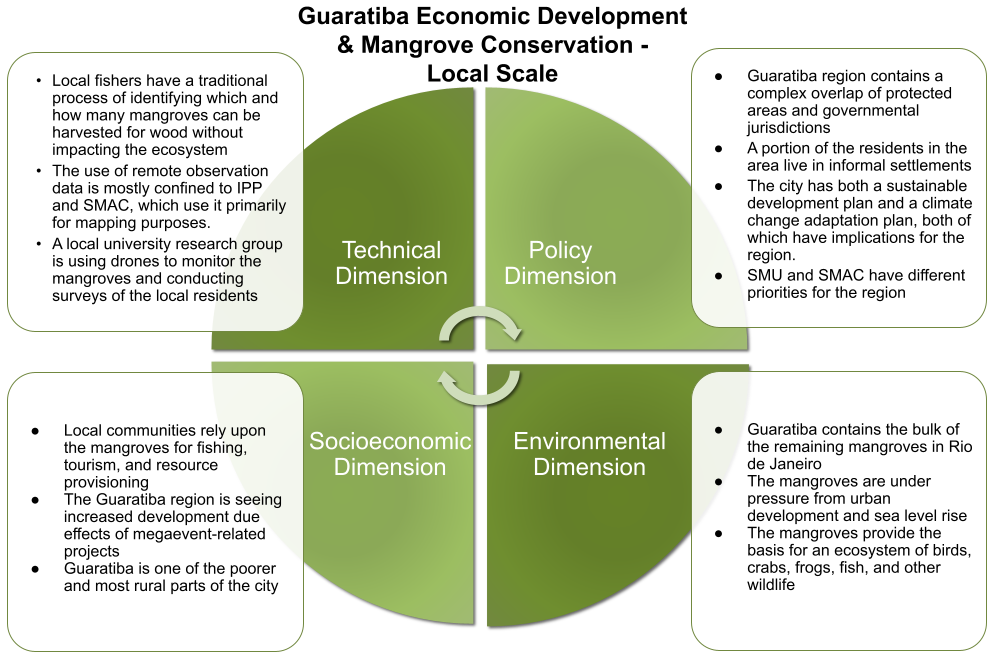
\includegraphics[width=0.8\textwidth]{Figures/chap4/dimensions_rio.png}
\caption[Rio de Janeiro System Context Dimensions]{Rio de Janeiro System Context Dimensions}
\label{fig:dimensions_rio}
\end{figure}

\paragraph{\hlc[green]{Big Plans and Megaevents in Rio de Janeiro}} \label{sec:rio-plans} \leavevmode\newline

Rio has a history of being on the forefront of intentionality and long-term strategic thinking when it comes to urban planning. In 1995, it became the first city in Latin America to develop a strategic plan, something it continues to do in three-year increments to this day \cite{prefeituradacidadedoriodejaneiroPLANOESTRATEGICOCIDADE2017}. Specific programs stemming from these plans include the Favela Bairro Programme which sought to upgrade the informal settlements and the Rio-Cidade Programa which sought to revitalize certain key areas of the city \cite{aciolyc.ReviewingUrbanRevitalisation2001}.

This type of strategic planning took place alongside a broader effort in the city and across Brazil to increase democratic participation in the planning process, as the country transitioned out of a military dictatorship \cite{aciolyc.ReviewingUrbanRevitalisation2001}. This interest in blending democracy with planning could also be seen in replacement of the government-owned Municipal Computer and Planning Company with the \ac{smu} and \ac{ipp}, thereby retaining both planning and data gathering capabilities, but putting them in the hands of government offices. While Rio has never reached the same level of public participation as Porto Alegre \cite{desousasantosParticipatoryBudgetingPorto1998}, this inclination has continued to today, as seen in efforts like the Data.Rio platform, which seeks to make increasing amounts of data about the city freely available online, and the proliferation of neighborhood-level``Associação De Moradores" (Residents' Associations).

Perhaps due to its beautiful natural environment and the importance of its tourist industry (a major focus of the 1995 strategic plan), Rio de Janeiro has long acknowledged the importance of environmental conservation and sustainability when it comes to development. Even prior to 1995, the city hosted the \ac{unced}, which gave birth to the Climate Change Convention, itself the basis for international climate change agreements. Twenty years later, the city would once again play host to such a conference, this time in the form of the 2012 \ac{uncsd}, which paved the way for the creation and adoption of the \acp{sdg} by the UN General Assembly three years later. It should be made clear that Rio de Janeiro was no mere picturesque venue for these conferences. Rather, the city has taken the UN pronouncements of sustainable development seriously, publishing a Climate Change Adaptation Strategy in 2016 (utilizing entirely intra-country expertise)  \cite{prefeituradacidadedoriodejaneiroClimateChangeAdaption2016} and a Resilience Strategy in 2017 (created in partnership with the Rockefeller Foundation) \cite{100resilientcitiesResilienceStrategyCity2017}. The city is currently using a participatory process to create a Sustainable Development Plan that will detail how the city intends to contribute towards the \acp{sdg} \cite{unitednationsbrazilONUConvidaCariocas2019}.

A plethora of plans does not necessarily result in smooth sailing, however (in fact, many would say that it is directly contrary to good development \cite{easterlyWhiteManBurden2007a}). While the climate and sustainability-related plans advocate for environmental protections, energy efficiency, and waste controls, the strategic plans have focused more strongly on economic development and the tourist industry, which is related to but not identical with environmental conservation. These latter plans have explicitly espoused the use of sports megaevents (which manifested in the form of the 2014 FIFA World Cup and the 2016 Summer Olympics) as a way of attracting investment \cite{sanchezMegaeventsUrbanRegeneration2013}, a pursuit that has arguably done little to advance either sustainable development or climate change resilience, particularly as many of the recent venues were built directly on waterfront or on protected nature reserves \cite{connorsLocalGolfersTest2016}. 

Of particular relevance to Guaratiba is how the megaevent-related development reshaped transportation patterns and commercial development throughout the city. This phenomena is perhaps best explained through the use of three maps. Figure \ref{fig:relocation} shows the origin and destination of most of the favela relocation efforts (both voluntary and mandatory) in the years leading up to the World Cup and Olympics. Most of the new settlements were constructed under the \ac{mcmv} program, a federal program started in 2009 that enabled the some of the poorest households in Brazil to purchase new homes with little-to-no down payments, interest rates of near-zero, and income-adjusted monthly payments. The program was initially aimed at building one million homes nationwide, then later expanded to three million, of which more than 100,000 were assigned to the city of Rio de Janeiro \cite{nadalMinhaCasaMinha2018}. The city partly used this allocation of federal funds to support favela relocation efforts as part of megaevent-related development.

\begin{figure}[!htb]
	\centering
	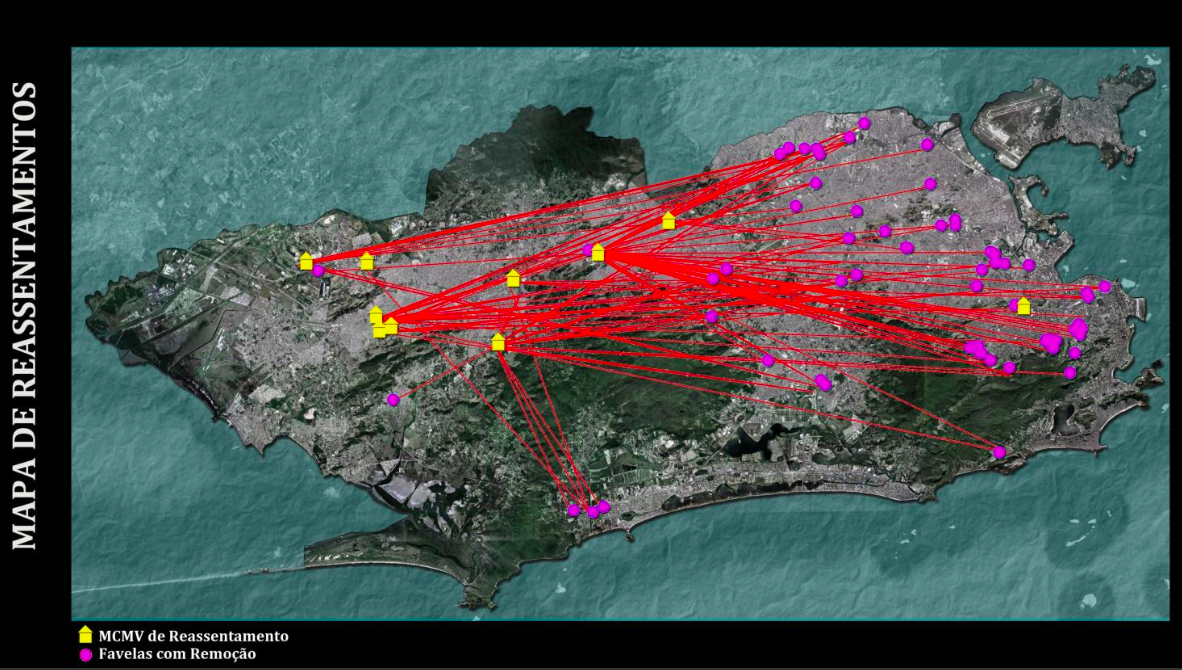
\includegraphics[scale=0.3]{Figures/chap4/Relocation.png}
	\caption[Favela Relocation Locations under MCMV between 2009 and 2013]{Favela Relocation Locations under \ac{mcmv} between 2009 and 2013. From \cite{faulhaberRioMaravilhaProjetos2012}}
	\label{fig:relocation}
\end{figure}

The relocation of favela inhabitants from east to northwest introduced problems, however. The original siting of informal settlements in Rio de Janeiro was partially driven by the availability of proximal employment. This is why historically, despite low land prices in the rural western parts of the city, most of the city's poor elected to live in high density favelas in the eastern, urban neighborhoods. Figure \ref{fig:employment} shows that while the new, formal \ac{mcmv} homes may have been higher quality than the old favela homes, they were also much further away from major centers of employment. Getting a nicer home is not much consolation for losing your job. 

\begin{figure}[!htb]
	\centering
	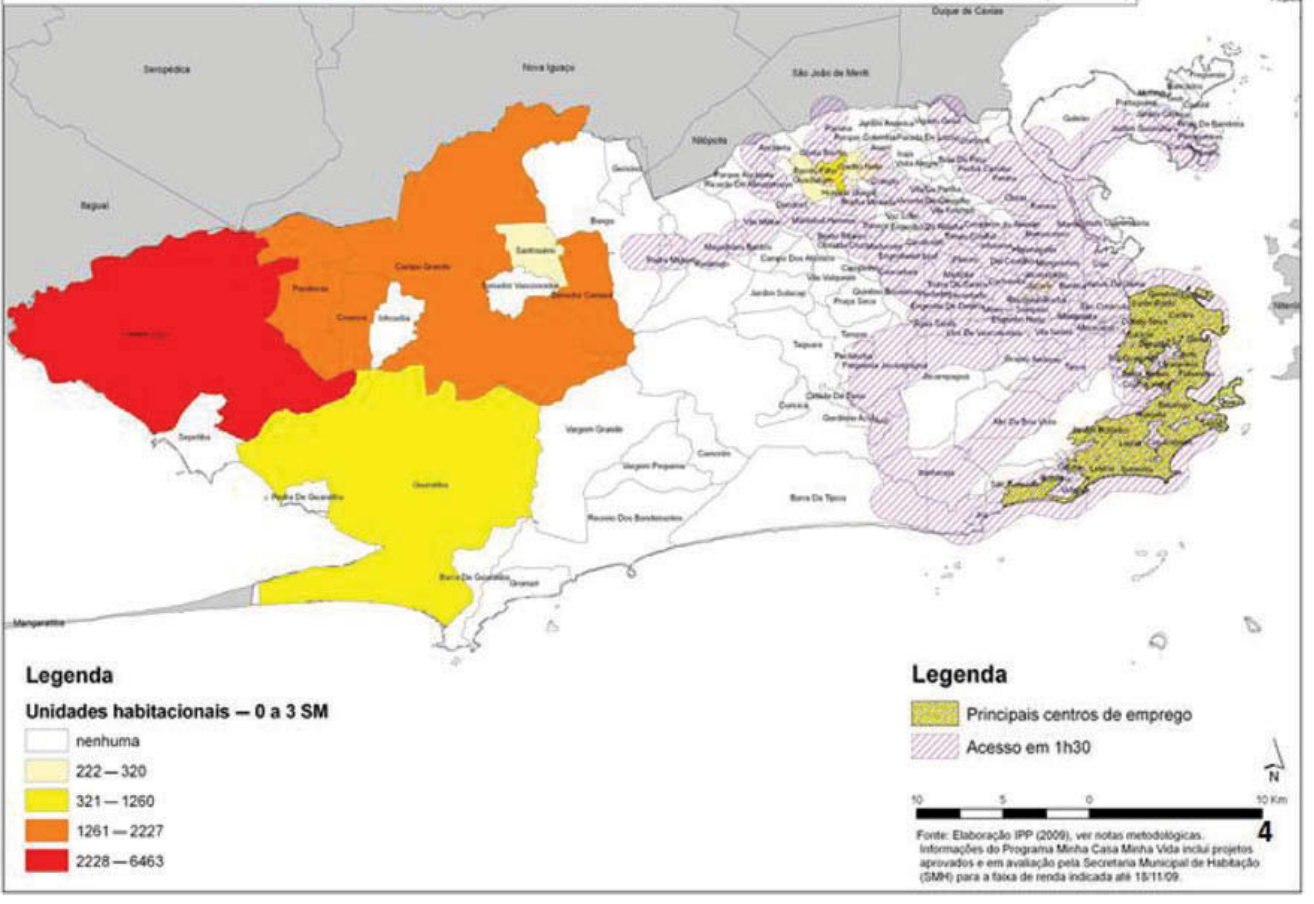
\includegraphics[scale=0.3]{Figures/chap4/Employment.png}
	\caption[Comparison of MCMV housing units and access to major employment centers.]{Comparison of MCMV housing units and access to major employment centers. From \cite{sanchezMegaeventsUrbanRegeneration2013}}
	\label{fig:employment}
\end{figure}

The Rio de Janeiro government was neither completely ignorant nor completely callous, however. As is common in the lead-up to sports megaevents, the city planned significant renovations, improvements, and extensions to the existing public transit system, as shown in Figure \ref{fig:transit}. Some of these, in particular the extension of the metro and the dedicated-lane bus Transoesto from Copacabana towards Barra Da Tijuca, were intended primarily to improve access to the major Olympic sporting venues. Many of the extensions, however were intended to better connect the northern and northwestern reaches of the city with the centers of employment, alleviating the concerns of those being relocated, while also improving accessibility for the existing residents of those areas. 

\begin{figure}[!htb]
	\centering
	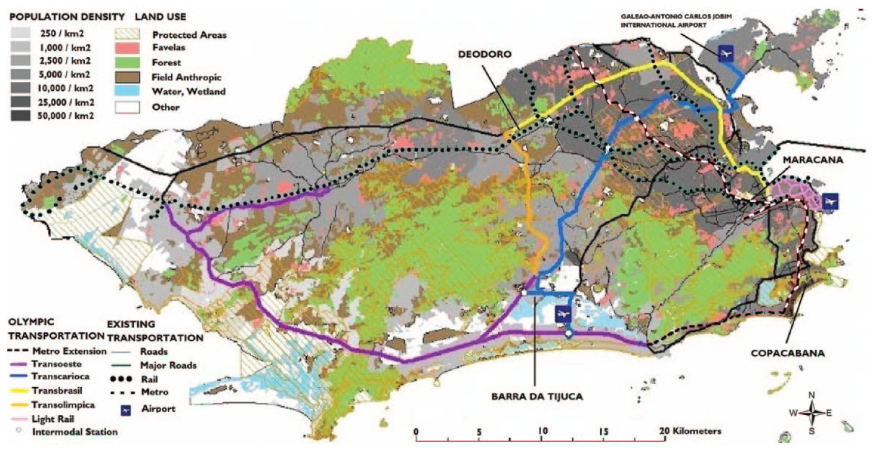
\includegraphics[scale=0.5]{Figures/chap4/Transit.png}
	\caption[Olympic-related transportation expansions and proximity to environmental protection areas]{Olympic-related transportation expansions and proximity to environmental protection areas. From \cite{kassens-noorOlympicTransportLegacies2018}}
	\label{fig:transit}
\end{figure}

Unfortunately the transit extensions were not as extensive, reliable, or high speed as initially promised \cite{wattsFuryFrustrationBrazil2014} and access to jobs for poorer communities ultimately decreased \cite{robertsonResultsAreCostly2017}. None of this directly impacted Guaratibans, however, as Guaratiba, tucked in the southwestern corner of the city, was neither the source nor destination of relocation efforts. What \textit{would} impact Guaratiba was the the Transoesto line and the related expansion of bus routes and road widths. These significantly increased the accessibility of downtown Rio de Janeiro for the largely rural Guaratibans (and vice versa). This accessibility significantly increased the value of the area for commercial activity and development, exacerbating ongoing local trends, as will be discussed further in Section \ref{sec:guaratiba-people}.

\paragraph{\hlc[green]{Overlapping Jurisdictions in Guaratiba}} \label{sec:rio-jurisdictions} \leavevmode\newline

While the city of Rio de Janeiro has busied itself with high-level plans, the municipal government is by no means the only government player in the city. Brazil has a whole has significant amounts of jurisdictional overlap between its municipal, state, and federal levels of government, when compared to countries such as the United States \cite{coutoImitationCoercionState2018}. This is particularly true for the city of Rio de Janeiro, which for more than 200 years until 1960, was the capital of Brazil. To this day, numerous institutions and roles within the city that elsewhere would be managed by the state or municipal governments are still federally administered. For example, there are numerous individual public schools, from primary through tertiary, that are run by either the city, state, or federal government, fairly independently of one another. In the field of environmental management, both the federal and state constitutions have chapters on the environment, and the municipality has its own an environmental secretariat. These distinct sources of authority are often visible in regulatory law, such as the separate endangered species lists maintained by the federal \cite{institutochicomendesdeconservacaodabiodiversidadeListaNacionalOficial2014} and state governments \cite{institutoestadualdoambienteListaEspeciesFauna}.

The most relevant aspect of these overlapping environmental jurisdictions when it comes to the Guaratiba area is the Carioca Mosaic\footnote{``Cariocan" is the demonym for inhabitants of Rio de Janeiro and ``Carioca" or ``Carioco" is an often-used adjectival form.}. This term refers to the federally-coordinated collection of federal, state, and municipal environmental conservation areas in the greater area of the city of Rio de Janeiro \cite{teixeiraPORTARIANo2452011}. Within the Mosaic, the federal government's \ac{icmbio} administers one national park and one national monument; the state government's \ac{inea} administers one state park, two environmental protection areas, and one biological reserve; and the municipal government's \ac{smac} administers 14 nature parks, two environmental protection areas, and a natural monument.

Of these various units, the following are in or in direct proximity to the Guaratiba area:

{\setstretch{1.0}
\begin{itemize}
	\item \ac{apa} Ambiental das Brisas (municipal)
	\item \ac{apa} da Orla da Baia de Sepetiba (municipal) 
	\item Parque Natural Municipal da Serra da Capoeira Grande (municipal)
	\item Parque Nacional Municipal da Prainha (municipal)
	\item Parque Nacional Municipal de Grumari (municipal)
	\item \ac{rbag}\footnote{Until 2006, this land was controlled by the nearby Brazilian Army \ac{ctex}, which continues to occupy a significant amount of land in the Guaratiba area and maintains some facilities within the \ac{rbag}. Similarly to other military administered lands in various parts of the world, \ac{ctex}'s control of this land results in a kind of quasi-environmental protection that is simultaneously less formally determined than actual environmental conservation areas but much more stringently enforced in practice. For example, there is an army vehicle workshop that disposes of waste directly into the mangroves, but commercial activities and unauthorized human access are strictly forbidden \cite{herzogGuaratibaVerdeSubsidios2009}.} (state)
	\item \ac{apa} Sepetiba II (state)
	\item Parque Estadual da Pedra Branca (state)
\end{itemize}}

This means that those who live and work in the Guaratiba area will regularly come into contact with eight different municipal and state-run conservation areas that are then collectively coordinated by the federal government. Such an arrangement has both benefits and costs. On the positive side, it can help ensure a certain minimum level of environmental protection amid shifting government priorities. For instance, at the time of writing, the state government of Rio de Janeiro is prioritizing security \cite{kaiserRioGovernorConfirms2019} while the federal government is actively scaling back environmental protections \cite{simoesBrazilBolsonaroEnvironment2019}. If one of these levels of government were solely in charge of environmental protection within the city of Rio de Janeiro, significant harm to the environment might occur, but since there are overlapping jurisdictions, the municipal government can continue to guarantee some minimum level of protections. Unfortunately, this system can (and does) not only lead to perhaps overly cumbersome permitting requirements for certain development projects, but can also lead to a diffusion of responsibility for environmental protections and inconsistent enforcement. 
 
This confusion of jurisdiction can have real consequences for residents of the area, particularly the disenfranchised. Take the case of Araçatiba, a small informal settlement almost completely surrounded by the \ac{rbag}. The favela ended up in its current position in the 1970s after commercial development (specifically television filming) pushed residents away from their previous location. At the time, this land was controlled by the Brazilian Army \ac{ctex}. In 2006, the \ac{ctex} transferred most of the land in this area to the state government to form the \ac{rbag} and to protect the local mangrove forests. Some additional land, including the Araçatiba informal settlement, was transferred to the civilian federal government. Over the next several years, the federal government took various measures to formalize the settlement, only to reverse course in 2014 and seek evictions instead \cite{chisholmWhoInvadingWhom2017}. The mayor at the time, Eduardo Paes, promised to prevent these evictions, but his successor did not follow suit, resulting in the demolition of several homes in 2017 and the threat of continued demolitions in the months to come \cite{stroblSOSAracatibaCommunity2018}. After protests organized by the favela residents, the federal government and \ac{inea} (the state environmental agency) apologized for the demolitions. Meanwhile, progress towards formal titling has stalled as it is dependent on homes being ``upgraded," which the city government has shown little interest in pursuing. Amid all of this is a somewhat bizarre digression that the federal government claimed that proper notice had been given prior to the demolitions via a message delivered to the president of the Araçatiba Residents Association, an organization that had not met in more than ten years \cite{stroblFourCoreCriticisms2018}. 

To summarize, the federal government tore down homes on federal land after being prevented for several years from doing so by the city government. The ensuing protests resulted in an apology by the state government and a refusal by the city government to certify the formalization of the settlement, which is still on federal land.

Of course, one favela is not necessarily representative of an entire region. The next two chapters will thus explore how the themes of this section and the previous section impact the people and environment of Guaratiba.

\paragraph{\hlc[cyan]{The Environment of Guaratiba}} \leavevmode\newline \label{sec:guaratiba-environment}

The distinguishing environmental aspect of the coastal Guaratiba area is its significant mangrove forest, made of five different mangrove species. Prior to colonization, most of the Rio de Janeiro coastal areas were either mountains or covered by mangroves. Over the centuries, the lowland mangrove forests were incrementally destroyed and filled in order to accommodate the growing city. The remaining mangrove trees of the greater Rio area, shown in Figure \ref{fig:mangrove-extent}\footnote{The methodology used to generate this and other original figures in the section are presented in Section \ref{sec:rio-evdt-e-method}.}, are confined primarily to northern Guanabara Bay (outside of the municipality) and eastern Sepetiba Bay (the bay on the western side of the city). This means that the Guaratiba forest, and the \ac{rbag} in particular, is the largest copse of mangroves within the city’s jurisdiction. These mangroves provide a variety of ecosystem services, including serving as a mechanism for highly efficient carbon sequestration, supporting a subsistence industry of fishing and crab catching (supporting vulnerable, juvenile shrimp in particular \cite{costaPensarMarPara1992}), preventing coastal erosion, and attracting a local ecotourism industry. Even these trees are under an ongoing threat.

\begin{figure}[!htb]
	\centering
	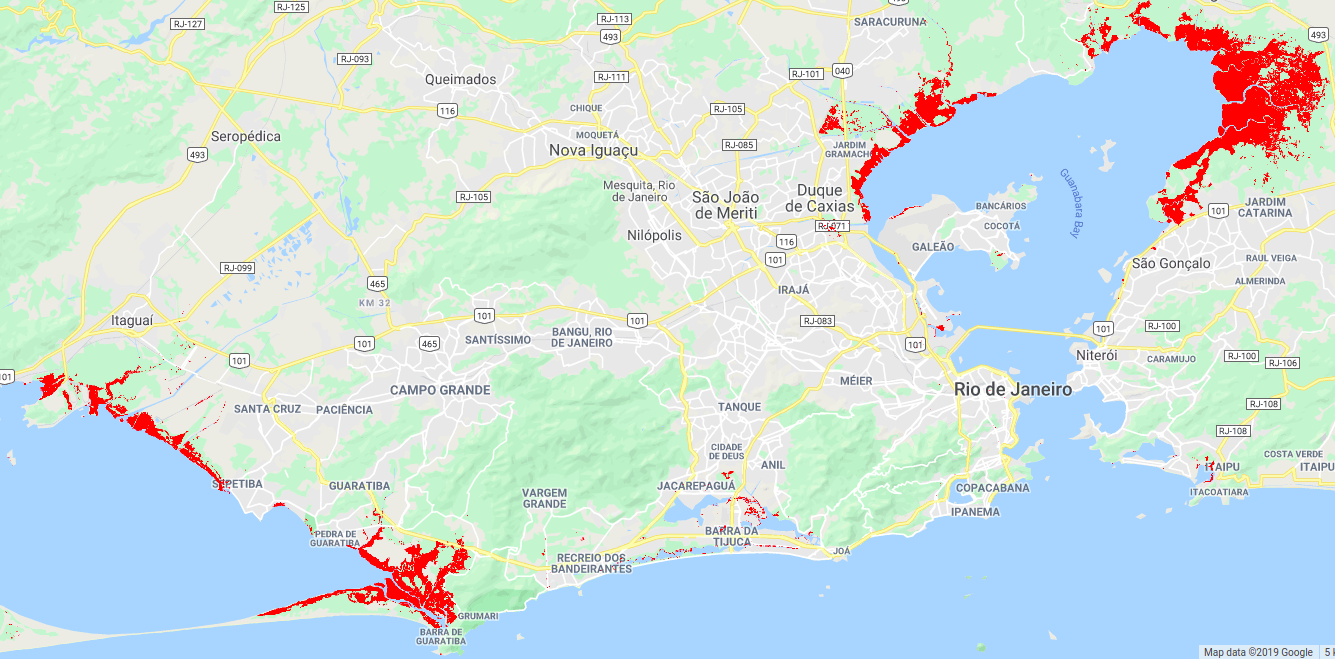
\includegraphics[scale=0.25]{Figures/chap4/MangroveExtent.png}
	\caption[Mangrove extent in the greater Rio de Janeiro area in 2018]{Mangrove extent in the greater Rio de Janeiro area in 2018, as estimated using a combination of Landsat, Sentinel, and PALSAR imagery.}
	\label{fig:mangrove-extent}
\end{figure}

Just up the cost from Pedra de Guaratiba, in the Santa Cruz \ac{ra}, the Ternium steel mill opened in 2010\footnote{Ternium purchased the steel mill in 2017. At its opening in 2010, the factory and associated port were operated by Thyssenküpp.}. This mill, along with its associated facilities, including an expanded canal, a bridge, a dam, and dredging of the bay directly replaced or caused the death of a significant number of mangroves (approximately 145 hectares) \cite{ecologusESTUDOIMPACTOAMBIENTALE2005}. Various indirect damages, including pollutants, silt disturbances, and changes in hydrology have resulted in further loses over the past several years \cite{lopesTerritorialidadesEmConflitos2013}. These effects are visible in the northwest corner of Figure \ref{fig:mangrove-ndvi-anomaly}. In this figure, red indicates damage to mangroves, including both decay and outright losses. Green indicates growth, both of existing trees and of new trees.

\begin{figure}[!htb]
	\centering
	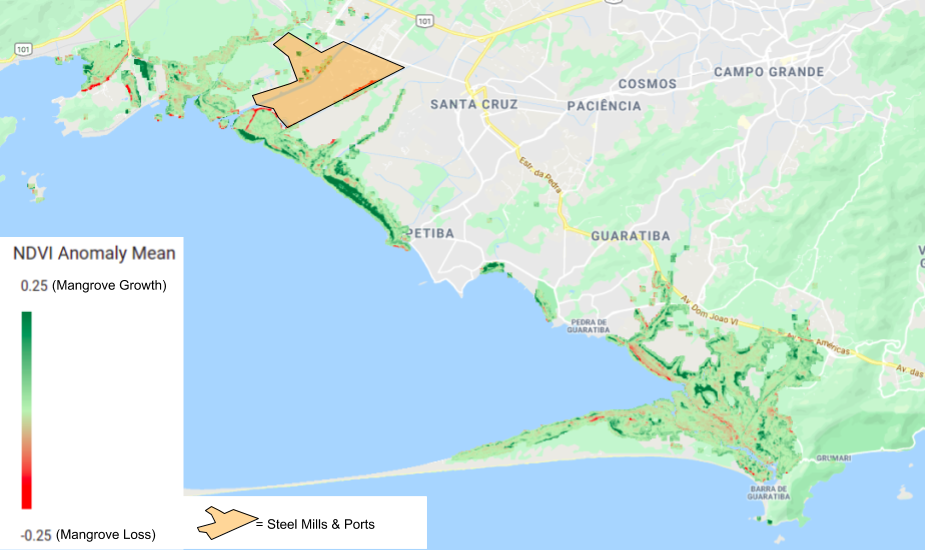
\includegraphics[scale=0.4]{Figures/chap4/NDVIanomaly_v2.png}
	\caption[Change in Guaratiba area mangrove health from 2000 to 2018]{Change in Guaratiba area mangrove health from 2000 to 2018, with the Gerdau Cosigua and Ternium steel mills indicated.}
	\label{fig:mangrove-ndvi-anomaly}
\end{figure}

While outside our direct area of interest, the steel mills of Santa Cruz have indirect effects on Guaratiba and are demonstrative of the results of potential industrial development further down the coast. In Guaratiba proper, the direct human-interfaces with the \ac{rbag} include \ac{ctex} in the center of the reserve, the Barra de Guaratiba neighborhood to the southeast, the Ilha de Guaratiba neighborhood\footnote{Ilha de Guaratiba is technically just a subdivision of Barra de Guaratiba. That said the two names are typically used to refer to different areas that have substantially different histories and economies and are only connected by a strip of land. Barra de Guaratiba is the urban cluster on the coast at the southern tip of the \ac{ra}. It was historically a fishing village and more recently a tourist destination. Ilha de Guaratiba, on the northern end of the official neighborhood along the highway, is a historical agricultural marketplace. The use of these names in this paper will stick to the common usage, particularly as we are more interested in the coastal regions rather than more inland areas such as Ilha de Guaratiba.} to the northeast, the Embrapa Agroindústria de Alimentos to the north, and the Araçatiba favela on the northeastern edge. Most of these areas are clearly visible in Figure \ref{fig:rbag}.

\begin{figure}[!htb]
	\centering
	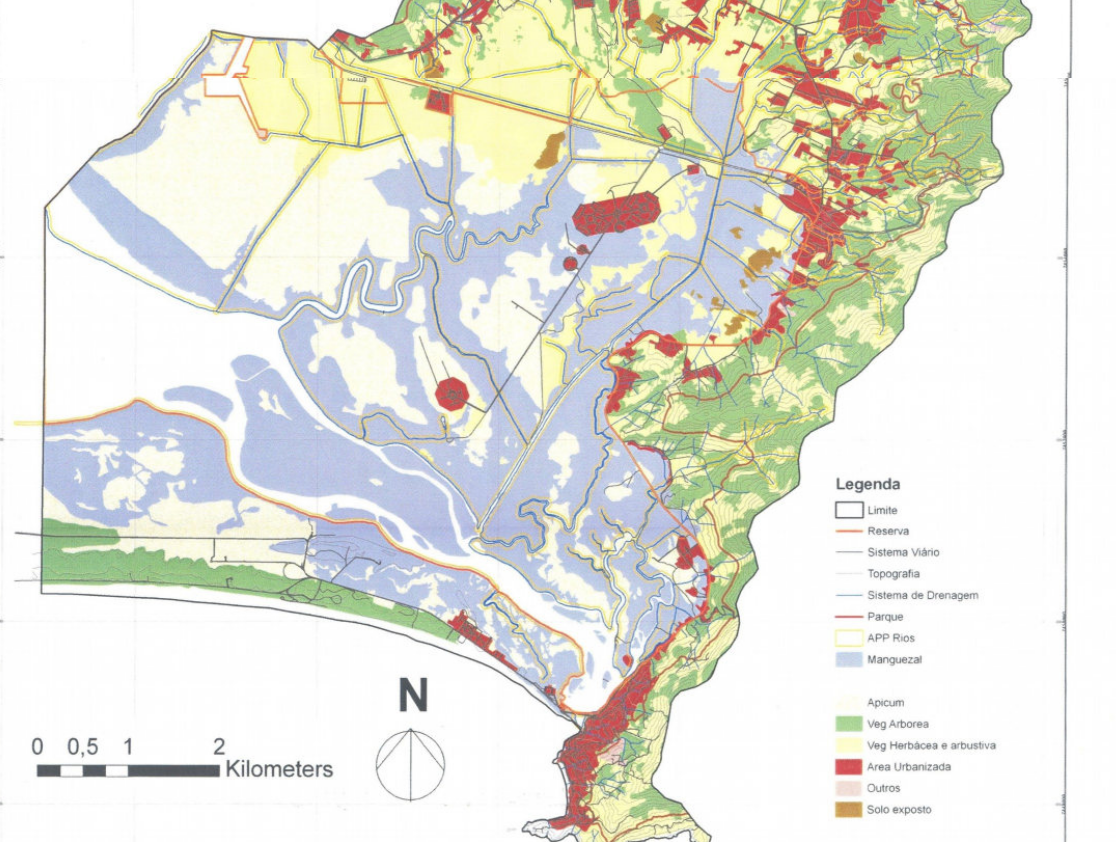
\includegraphics[scale=0.3]{Figures/chap4/RBAG.png}
	\caption[Map of RBAG and nearby urbanization]{Map of RBAG and nearby urbanization. Excerpted from \cite{herzogGuaratibaVerdeSubsidios2009} and originally made by IPP.}
	\label{fig:rbag}
\end{figure}

The health of the \ac{rbag} mangroves is a mixed bag. There has been some damage to certain sections of the forest, partly due to an invasive insect species and partly due to the increased sewage flows created by an increasing population and increased commercial activity. The dumping of waste in informal landfills, even when outside the mangrove forest itself, can still cause damage, as flows of water can be diverted or blocked, killing off sections of mangroves \cite{castroOSDESAFIOSPLANEJAMENTO2012}. All of this is driven by the fact that while there are significant legal environmental protections within \ac{rbag}, there are essentially no restrictions on development and activity just outside of the reserve, despite the fact that the mangrove forest occupies one of the primary outlets of regional drainage basin.

One component of the mangrove forest that is most directly threatened by commercial development are not the mangroves themselves, but the \textit{apicun}, hyper-saline mudflats created by the mangroves in various places on the interior and edge of the forest. These flats provide a variety of important ecological functions, such as serving as migratory stops and breeding grounds for thirty-nine species of birds\footnote{It is perhaps worth mentioning that this number used to be higher. For instance, Guaratiba takes its name for the local word for the scarlet ibis bird: \textit{guarás}. This bird is no longer found in the Rio de Janeiro area, pushed out due to a declining availability of its preferred habitat, the mangroves.} and homes for twelve species of crabs (a major target of local fishers) \cite{vicenteAvaliacaoHidrogeologicaRegioes2010}. They also represent a of land that the mangroves spread into when pressured from other directions. Despite these important functions, the apicuns are not as well protected as the mangroves themselves under the law and are commonly viewed by the public as wasted land that serves no purpose and thus ripe for development.

Additionally, part of the aforementioned transit expansion efforts was the construction of the first highway through the region, Av. D. João VI. This highways has isolated a section of mangrove forest from the main \ac{rbag} with implications that are yet to be seen. One key consequence of the highway is that the mangroves no longer have a mechanism for moving inland in the face of seaward pressures, such as a rising sea level that may take place over the coming decades.

\paragraph{\hlc[green]{The People of Guaratiba}} \label{sec:guaratiba-people} \leavevmode\newline

Guaratiba has historically had such a small population largely been due to its relative isolation. Separated by mountains on the east from the primary urban core and on the north from the more heavily populated Campo Grande \ac{ra}, Guaratiba is largely rural and heavily forested. Since the decline of colonial-era plantation farming, the residents have primarily engaged in subsistence and near-subsistence commercial activities, including artisanal fishing, farming, and ranching (including of frogs). The products of this economic activity were typically sold (via local distributors) in outdoor markets (called \textit{fieras}) throughout the Rio de Janeiro city. This largely informal supply chain kept residents somewhat isolated from the globalized agricultural markets that drove industrial farming in other parts of the city \cite{fernandesDecodificandoGeografiasPreteritas2010}.

By most development metrics, the inhabitants are some of the worst off in Rio de Janeiro, with low rates of education, more children per family, and poor health. An example of the latter can be found in the fact that approximately a quarter of the dogs in the area carry \ac{avl}, a typically fatal parasite, and human cases are relatively common, particularly in the Barra de Guaratiba area, despite control efforts \cite{cabreraCanineVisceralLeishmaniasis2003}. Over the past few decades, however, the the area has been experiencing rapid growth recently, significantly outpacing the city as a whole \cite{pizzolatoLOCALIZACAOESCOLASPUBLICAS2013}. Much of this was driven by increasing industrial employment opportunities in Campo Grande and Santa Cruz, to the north, of which the aforementioned steel mills are just one example. These areas have historically been significantly easier to reach than the core of Rio de Janeiro to the east. The more recent transit expansion projects have accelerated this trend, enabling easier access to Campo Grande and Santa Cruz. The improved connections eastward have also allowed for a more substantial ecotourism industry focused on the coastal mangrove forests and for a more substantial regional tourism (i.e. tourists from other parts or Rio de Janeiro) spending the weekends at the beaches of the area. These latter tourists have also begun purchasing second homes (vacation homes) in the area, particularly in Barra de Guaratiba, driving commercial development of condominiums and restaurants \cite{herzogGuaratibaVerdeSubsidios2009}. Such condominiums first entered the Guaratiba \ac{ra} in the 1990s and have spread to Barra de Guaratiba in the past 15 years, as transportation infrastructure to the peninsula has improved \cite{fernandesDecodificandoGeografiasPreteritas2010}. 

Such growth has itself introduced certain additional problems. The area was already characterized by low levels of education (4.7 years of school on average, by some estimates), and the increased population seems likely to overwhelm the existing school system, an issue further complicated by the fact that, due to the rural nature of the region, many students are already more than three kilometers from the nearest school and thus cannot easily be reassigned to further, emptier schools. One analysis of the \ac{ra} estimated a deficit of nearly 35,000 seats by 2020, despite low rates of attendance \cite{pizzolatoLOCALIZACAOESCOLASPUBLICAS2013}. One issue is that there are few mechanisms for community organization in the area. As mentioned earlier, Araçatiba did have a Residents Association, only for it to dissolve more than ten years ago. Now they find themselves trying to work with a city-wide Conselho Popular to effectively advocate for themselves \cite{stroblFourCoreCriticisms2018}. Even the more formal neighborhoods of Guaratiba typically have either ineffectual or nonexistent associations \cite{herzogGuaratibaVerdeSubsidios2009}. On the economic rather than residential side, frog ranchers are virtually solitary \cite{borinUMAABORDAGEMASSOCIATIVISMO2013}, as are many of the farmers. Perhaps the primary organized group in the area are the artisanal fisherman, who participate in a variety of local and regional associations of varying degrees of formality \cite{lopesTerritorialidadesEmConflitos2013}.

The continued commercial and industrial development threatens to displace many of the historical communities of Guaratiba. In the 1970s, Araçatiba was created after informal settlements were forced to move by a film studio. More recently, the opening of the Ternium steel mill, in addition to its environmental impacts discussed earlier, effectively excluded artisanal fishing activities in a significant portion of the Sepetiba Bay. While the effects of this are more directly born by neighboring Sepetiba, fishers from that area have been forced eastwards, thereby impacting Guaratiba fisherman, particularly the approximately 1,000 fishers who reside in Pedra de Guaratiba \cite{lopesTerritorialidadesEmConflitos2013}. These fishers are also pressured due to technological adoption by the more large-scale, commercial fishers. The increasing prevalence of industrial trawl fishing over the past few decades in the Sepetiba Bay (instead of more targeted, historical fishing methods), has resulted in the increased catching of juvenile and unintended fauna, as well as stirring up the silt on the bottom of the bay. This has led to increased tensions and conflicts between the the industrial and artisanal fishers \cite{begossiMappingSpotsFishing2001}, somewhat attenuated by the (illegal) ability of the artisanal fishers to operate inside the mangrove forests. This ability is by no means guaranteed, however. Fishing is nominally prohibited within the \ac{rbag}. This prohibition is currently rather poorly enforced, as part of a more board set of allowances provided to local (typically informal) residents. Another example of this allowance is that the bounds of the \ac{rbag} have, during each update, been intentionally drawn to exclude existing settlements \cite{castroOSDESAFIOSPLANEJAMENTO2012}. That said, a future policy change could result stricter enforcement and in yet further encroachment on locals’ means of subsistence. 

As Guaratiba has become more connected to the rest of the city and commercial interests have increasingly moved in, small-scale farmers have been negatively impacted as well as the fishers. The open-air fieras have been increasingly replaced by supermarkets, depriving the farmers of a means of selling their produce. Many of the farmers adapted by switching from food produce to ornamental plants, something that Guaratiba has developed a reputation for over the past several decades \cite{fernandesDecodificandoGeografiasPreteritas2010}. 

All of this is to say that isolated, rural, and poor Guaratiba be none of these things before too long. But will the Guaratibans benefit or merely be replaced? And what will happen to the natural environment that has supported them for so many generations?

The following section will take a look at the relationships between stakeholders with a more specific focus.

\subsubsection{\hlc[cyan]{Analyze System Stakeholders}}

There are multiple ways to consider the relevant stakeholders and their relationships. One is to separate government stakeholders from non-government stakeholders. With regards to the former, as discussed in Section \ref{sec:rio-jurisdictions}, Rio de Janeiro's complicated history has resulted in a plethora of ministries with overlapping jurisdictions. Figure \ref{fig:government-agencies} summarize the most relevant municipal, state, and federal ministries, institutions, and initiatives. Each of these institution direct own and manage certain parcels of land within the city of Rio de Janeiro (not necessarily within this project's study area) in addition to regulating certain activities throughout the municipality. While they do certainly communicate and coordinate, their priorities are not necessarily in alignment (as will be discussed in the next section). 


\begin{figure}[!htb] 
\centering
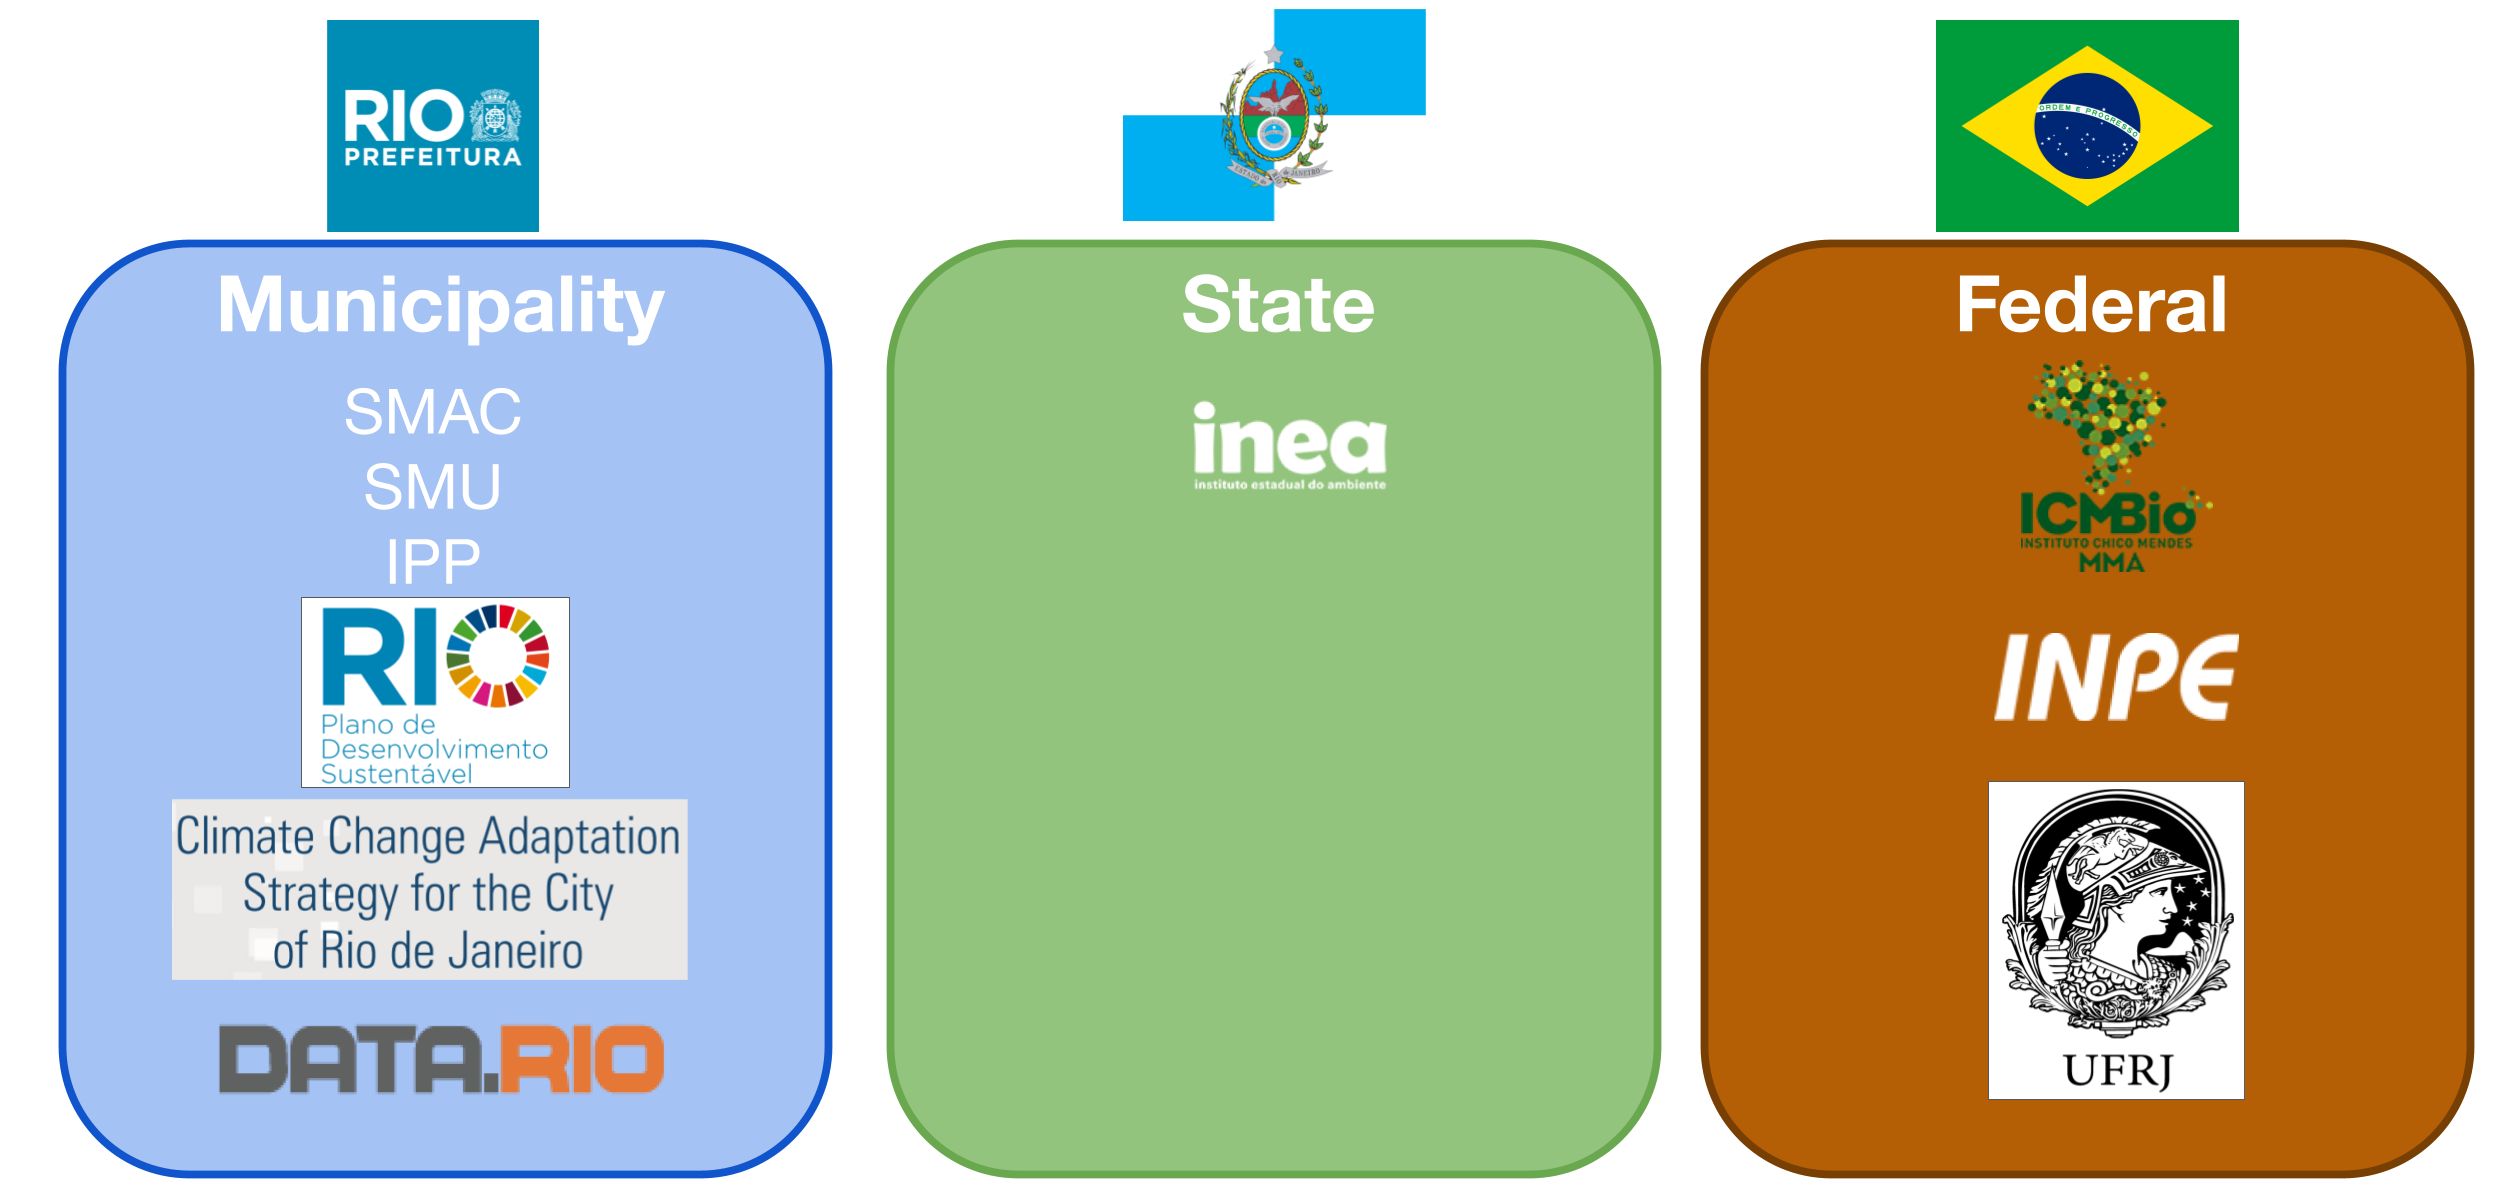
\includegraphics[width=0.8\textwidth]{Figures/chap4/government-agencies.png}
\caption[Relevant government stakeholders in Rio de Janeiro case study]{Relevant government stakeholders in Rio de Janeiro case study, organized from left to right as municipal, state, and national.}
\label{fig:government-agencies}
\end{figure}

The non-government actors include local actors such as residents (and their associations) and commercial developers. These are the stakeholders most directly impacted by land use decisions and the health of the mangroves.

We can also analyze the stakeholders is by classifying them into primary-secondary-tertiary categories or mapping their relationships. Figure \ref{fig:rio_stakemap} does both of these simultaneously. The arrows between each stakeholder represent the means by which they influence one another. This can include direct orders or voicing of opinion (such as legislative policy), knowledge or information (such as information about the state of the mangroves), or tangible benefits (such as money, goods, or services).

The primary stakeholders, marked in blue, represent those that have the most direct land use decision-making power in the study area. This is expressed both through land ownership/control and through policy regulations. The Pescadors / Local Residents Association is represented with a gradient as some members of this category manage land and some do not, or only do so in a legally precarious manner, such as the residents of the Araçatiba informal settlement. 

The yellow boxes represent the secondary stakeholders, who advice and influence the primary stakeholders through information, funding, or policies. The municipal, state, and federal legislative bodies play important roles in translating the perspectives of their constituents into directives for the various ministries and secretariats. The scientific community and \ac{ipp} meanwhile provide the knowledge and information that shapes how these directives are carried out. The Space Enabled Research Group resides in this category, as the project is aimed at supporting decisions of the various primary stakeholders. 

Finally the tertiary stakeholders are shown in red and include those who impacted by land use decisions and the health of the mangroves but who do not directly participate in decision-making. This includes some of the local fishers and residents who may not own land but still derive their living from it, as well as the global community who benefits from both ecotourism to the mangroves and from the carbon storage and sequestration that the mangroves provide.

While not common to stakeholder mapping, I chose to represent that mangrove forests and other land of the study area as a stakeholder, albeit one outside of the primary-secondary-tertiary classification system. This is done for two reasons. First, it raise the profile of the environment from a mere incidental provider of human benefits to something worth direct recognition. Second, many of the relationships between the stakeholders are indirect, mediated through land use decisions and the mangrove forests themselves. Such relationships are difficult to map without including the land itself as a stakeholder.

\begin{figure}[!htb]
	\centering
	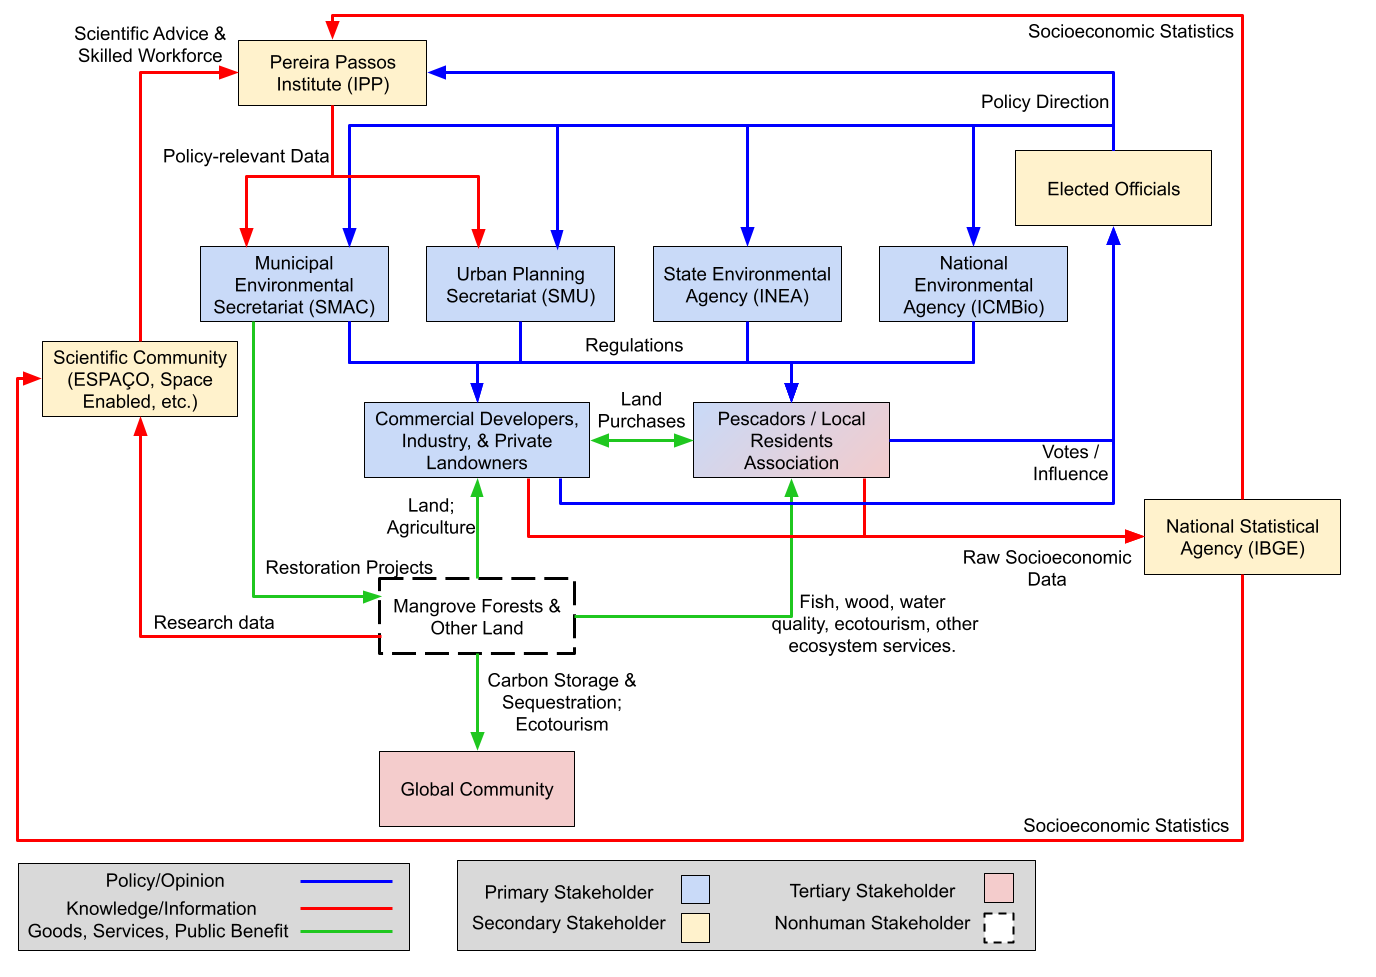
\includegraphics[width=0.9\textwidth]{Figures/chap4/Stakeholder_Map.png}
	\caption[Stakeholder Map for the Mangrove Forests of Rio de Janeiro]{Stakeholder Map for the Mangrove Forests of Rio de Janeiro}
	\label{fig:rio_stakemap}
\end{figure}

It should be noted that Figure \ref{fig:rio_stakemap} represents a descriptive perspective, focuses on land use decision-making. If one wanted to construct a map centered on this project's \ac{evdt} \ac{dss}, the map would differ significantly. For instance, the primary stakeholders would be the Space Enabled Research Group and \ac{ipp}, as those with the most direct involvement in the creation of the \ac{dss} (despite efforts to broaden the circle of collaboration wider). I did not think such a map was necessary to develop the System Objectives in the next section, but other case studies may find such a practice useful.

\subsubsection{\hlc[cyan]{Understand Desired Outcomes \& Objectives}} \label{sec:rio-saf-objectives-result}

Based on both the literature survey and the interviews/meetings with stakeholders, I derived a set of key stakeholder's Needs, Desired Outcomes, and potential System Objectives, which are summarized below in Table \ref{tab:rio-needs}. The \ac{dss} will not address all of these but will be informed by them. This table, in conjunction with the stakeholder classification and mapping in the previous section, allowed for the identification of both shared and conflicting objectives. For example, a formal sewage system was noted as a priority by both the urban-planning-oriented \ac{smu} and the environment-oriented \ac{smac}. Notably this was not brought up by the fishers themselves (though it should be noted that I did not directly ask them about it either). 

In general, conservation and even replanting of the mangroves was a common Desired Outcome, but the reasoning and priority for this varied significantly, resulting in important differences. The fishers prioritized preservation of existing mangroves and replanting in recently deforested areas. They viewed city efforts to compensate for development-induced deforestation with replanting efforts elsewhere (including in areas deforested decades or centuries ago) as irrelevant to their needs. 

All of these key stakeholders were in agreement that improved understanding of mangrove ecosystem services would assist their decision-making and enable them to better argue for their interests.  

Though not included in the table, \ac{icmbio}'s Needs, Desired Outcomes, and System Objectives were similar to those of \ac{smac}. It is also reasonable to suppose that \ac{inea}'s interests are similar (though certainly not identical) to those \ac{smac} and \ac{icmbio}.

\begin{landscape}
\begin{table}[t]
\caption[Needs, Outcomes, and Objectives for Rio de Janeiro Case Study]{Stakeholder Needs, Desired Outcomes, and potential System Objectives for key stakeholders in the Rio de Janeiro Case Study}
\label{tab:rio-needs}
\begin{center}
\scriptsize
\begin{tabular}{| C{2cm} |  L{5.33cm} | L{5.33cm} | L{5.33cm} |} \hline
 
\textbf{Stakeholder Group} & \textbf{Stakeholder Needs} & \textbf{Desired Outcomes}  & \textbf{Potential System Objectives} \\ \hlinewd{2pt}


\multirow{2}{*}{\centering Fishers} & \tabitem{Access to fish and wood in their historical locations} & \tabitem{Ability to conduct sustainable wood harvesting in the mangrove forests} & \tabitem{Support/justify mangrove preservation and restoration} \\ 
 & \tabitem{Water access for boat storage and repair} & \tabitem{Preservation/restoration of existing mangroves} & \\ \hline



\multirow{5}{*}{\centering \ac{smu}} & \tabitem{Improved water quality and waste removal} & \tabitem{Formal sewage system} &  \tabitem{Support/justify zoning decisions}\\

& \tabitem{Minimize gentrification} & \tabitem{Controlled drainage} & \tabitem{Inform sewage system project prioritization}\\

& \tabitem{Encourage economic development and increased standard of living in area}  & \tabitem{Facilitate formalization of informal settlements} & \tabitem{Improve understanding of ecotourism in region}\\ 

& \tabitem{Reduced flood risk} & \tabitem{Reduce sediment accumulation}  & \\

&  & \tabitem{Economic connections/commuting to Campo Grande, not downtown Rio} & \\ \hline




\multirow{5}{*}{\centering \ac{smac}} & \tabitem{Conservation of environment and biodiversity} & \tabitem{Protection of both mangroves and wetlands} & \tabitem{Inform definition of conservation unit boundaries} \\ 

& \tabitem{Improved water quality} & \tabitem{Replanting/restoration of mangroves across the city} & \tabitem{Support/justify mangrove preservation and restoration} \\

& \tabitem{Improved air quality} & \tabitem{Formal sewage system} & \tabitem{Inform targeting of new parks or replanting projects} \\

& \tabitem{Sequestration of carbon} & \tabitem{Protection of riparian areas} & \tabitem{\ac{eo} data use capacity building} \\

& \tabitem{Real time \& local scale environmental data} & \tabitem{Better use of \ac{eo} data} & \\ \hline




\ac{ipp} & \tabitem{Ability to inform other municipal agencies} & \tabitem{Better socioenvironmental data/metrics} & \tabitem{Complex systems capacity building} \\

& \tabitem{Understand future changes/threats} & \tabitem{Method for generating future scenarios, particularly climate change} & \tabitem{Scenario planning capacity building} \\ \hline

\end{tabular}
\end{center}
\end{table}
\end{landscape}

\subsubsection{\hlc[cyan]{Select System Functions}}

Based on the above analysis, several \ac{dss} system functions were selected. These are:

\begin{itemize}[itemsep=0pt,parsep=0pt]
    \item{\textbf{Descriptively model environmental phenomena}, in particular mangrove health trends over the past two decades. This will inform the current state of the environment and possible future trajectories.}
    \item{\textbf{Provide estimates of mangrove ecosystem services}, including both local and global services. This will help inform decision-making around mangroves by various stakeholders.}
    \item{\textbf{Generate potential future conservation scenarios.}}
\end{itemize}

In addition to these \ac{dss}-specific functions, there are some additional functions to be performed by the Space Enabled - \ac{ipp} collaboration on this project, namely:

\begin{itemize}[itemsep=0pt,parsep=0pt]
    \item{\textbf{Modeling and \ac{dss} development capacity building.} This is primarily relevant to \ac{ipp}.}
    \item{\textbf{\ac{eo} analysis capacity building.} This is most relevant to \ac{smac}, but \ac{smu} has also expressed such an interest.}
\end{itemize}


\subsubsection{\hlc[cyan]{Assign Function to Forms}}

The particular form decided to implement these functions was a desktop-based data visualization and exploration tool. A desktop-based system, rather than an online or mobile system, was chosen for a few reasons. First, familiarity with non-phone computers and internet access varies significantly among the stakeholders. If an online version was developed, it would need to be easily accessible and intelligible on a mobile device. This was beyond the abilities of myself and other teammates, though it remains an option for the future. The preferred alternative was a desktop-based system that would be intended for use in workshops with stakeholders, rather than for independent use, thereby reducing those barriers of entry. This decision is not without its flaws, as discussed in Section \ref{sec:rio-discussion}. 

The above \ac{saf} results are summarized in Figure \ref{fig:system-diagram-rio}. The rest of the chapter will detail the development of \ac{dss}, along with the models underlying it, before returning to the question of how well the resultant system fulfilled this vision.

\begin{figure}[!htb] 
\centering
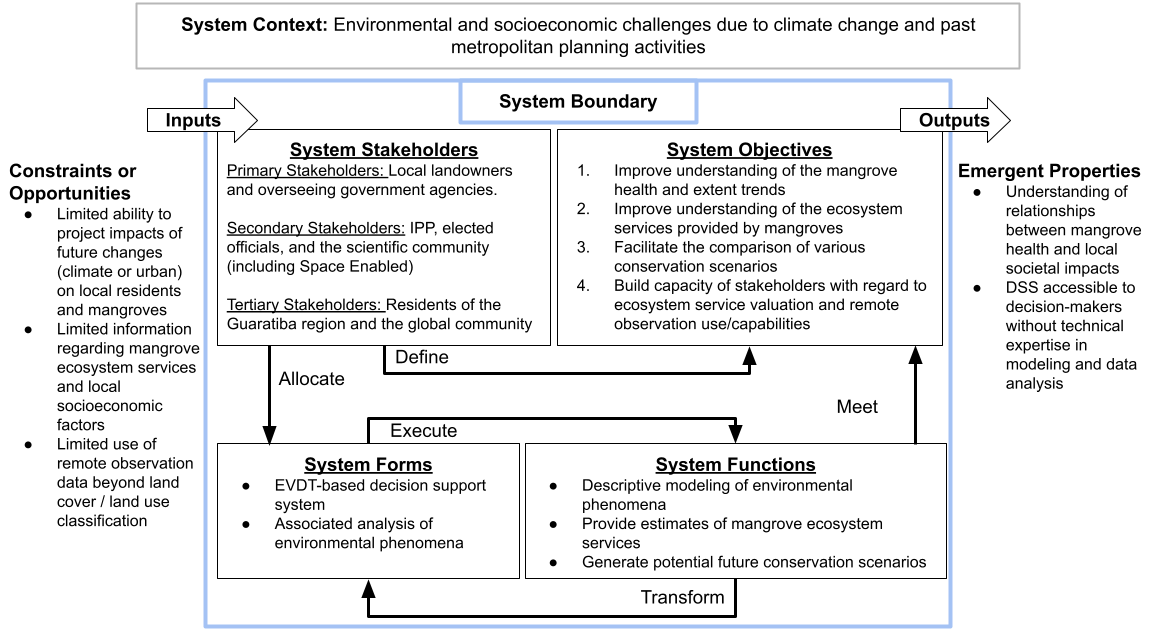
\includegraphics[width=0.8\textwidth]{Figures/chap4/system-diagram-rio.png}
\caption[High level Systems Architecture Framework diagram for the Rio de Janeiro case study]{High level \ac{saf} diagram for the Rio de Janeiro case study}
\label{fig:system-diagram-rio}
\end{figure}

This was not the only form considered. For example, Figure \ref{fig:concept_flow} shows two potential user experience concepts for a \ac{dss}. Each is aimed primarily at the needs of a particular stakeholder group. Ultimately the selected form was essentially the left option as it satisfied the needs of more of the involved stakeholders. 

\begin{figure}[H] 
\centering
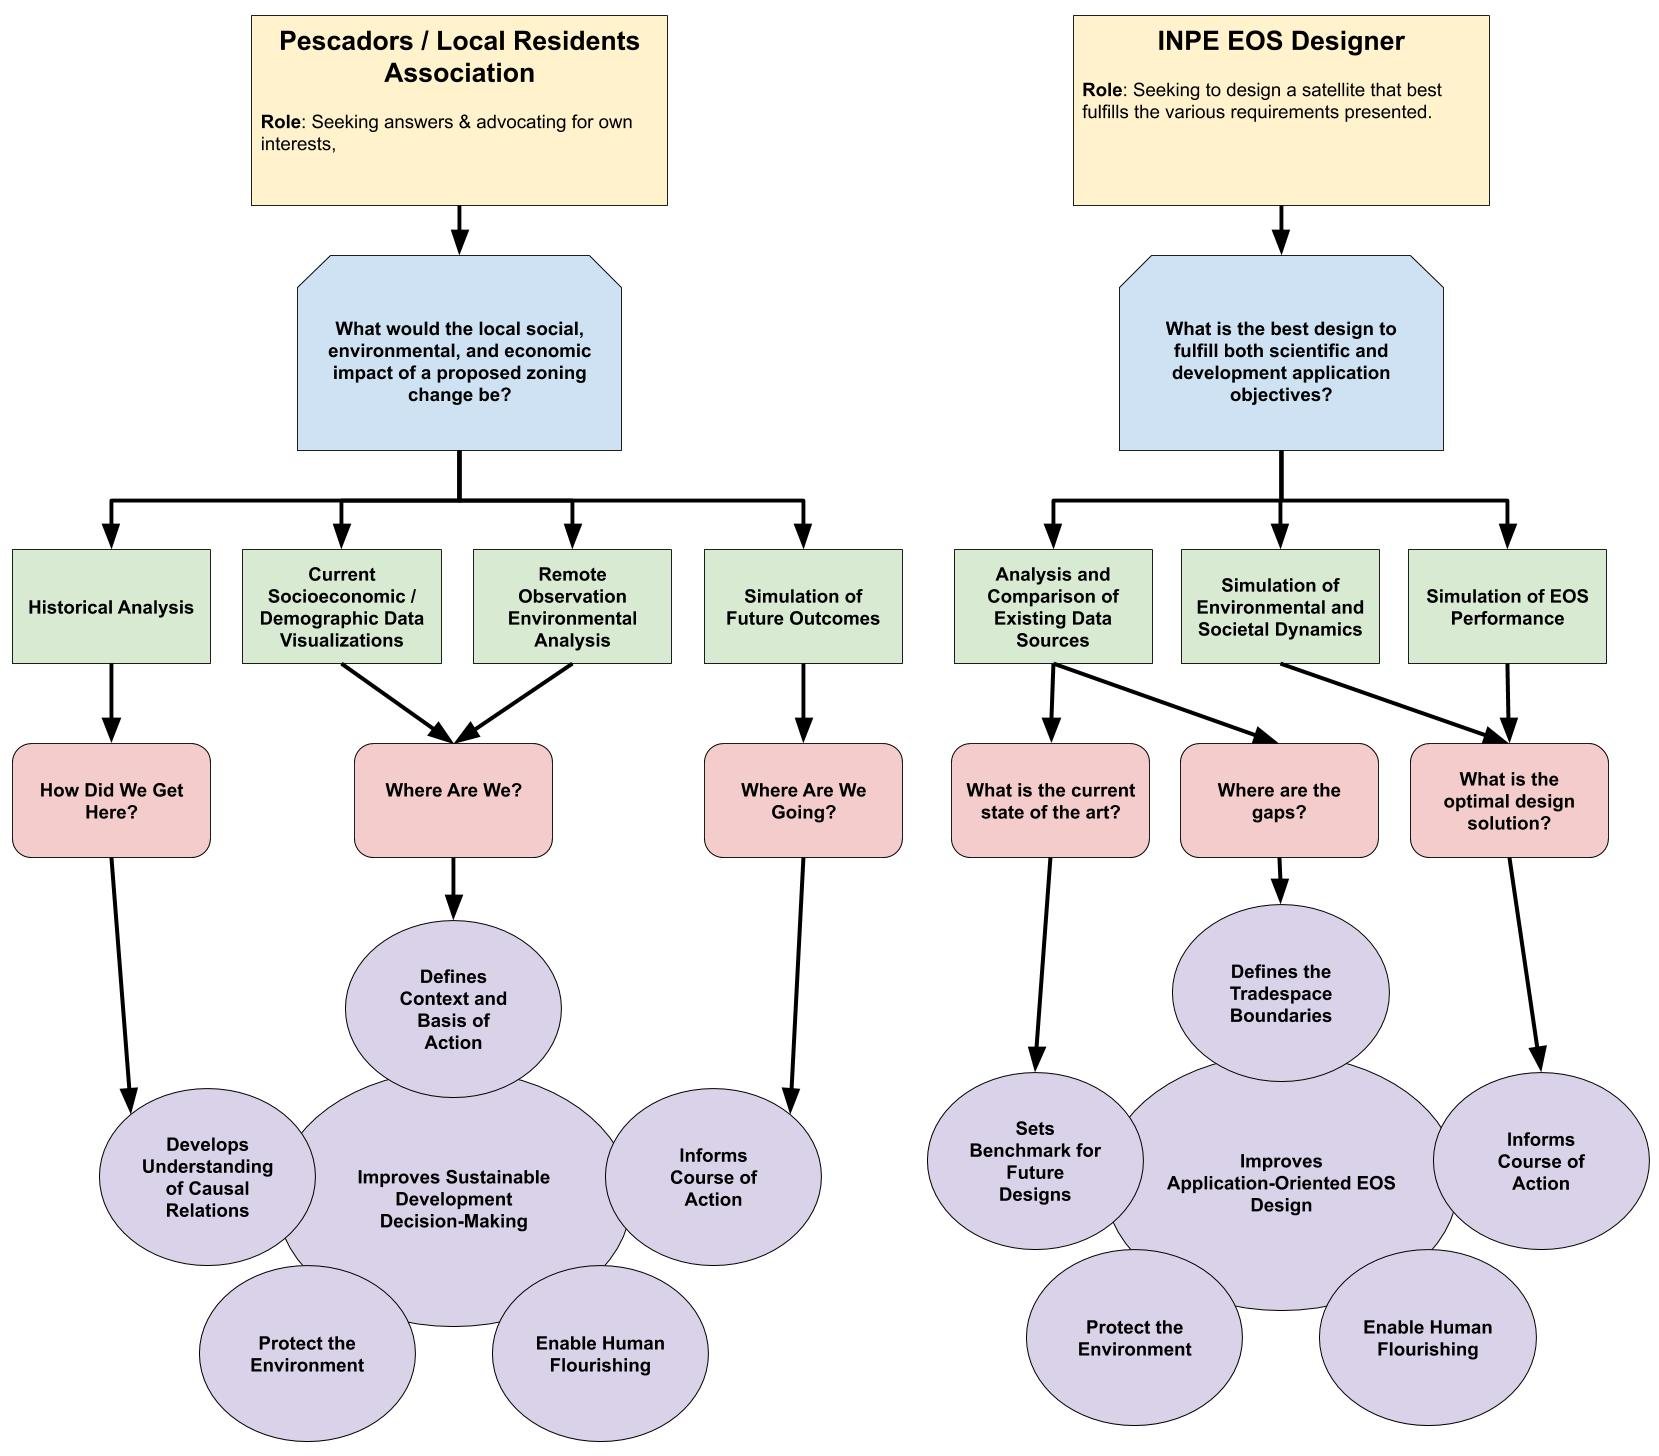
\includegraphics[width=0.9\textwidth]{Figures/chap4/concept_flow.jpg}
\caption[Two potential user experience concepts for the Rio de Janeiro case study]{Two potential user experience concepts for this case study}
\label{fig:concept_flow}
\end{figure}

\subsubsection{\hlc[cyan]{Monitor and Evaluate Systems}}

As was stated in Section \ref{sec:rio-monitor-method}, long-term monitoring of the Guaratiba environment or the impacts of this project are beyond the scope of this thesis. Instead, feedback from a subset of the stakeholders was relied upon. This feedback is only intelligible in the context of the resulting \ac{dss}, so it is reported later in this chapter, in Section \ref{sec:rio-dss}.

\section{\hlc[cyan]{EVDT Application}} \label{sec:rio-evdt}

The following subsections walk through the components of the system from an \acf{evdt} perspective, detailing what models were used and the results of those models. Before proceeding though, it is worth stating what exactly each of the four components of \ac{evdt} mean for this system. Returning to the four questions from Section \ref{sec:evdt-questions}, we ask the following:

\begin{enumerate}[itemsep=0pt,parsep=0pt]
	\item \textbf{What is happening in the natural environment?} What are the impacts of seal-level rise and urban expansion on the mangrove forests? What role do complex secondary factors such as sedimentation change due to land use conversion and organic discharge due to agricultural activities, play in determining mangrove growth? 
	\item \textbf{How will humans be impacted by what is happening in the natural environment?} What impact do the designation of natural reserves have on the community? What effects would the lack of mangroves have on the city? What is the value of the carbon sink of mangrove forests?
	\item \textbf{What decisions are humans making in response to environmental factors and why?} How are planning policies such as restricted land use conversion in certain protected natural reserves developed? How are other centralized and decentralized decisions made, such as the rate of urban expansion or the development of transportation infrastructure? 
	\item \textbf{What technology system can be designed to provide high quality information that supports human decision making?} What satellite, aerial, and in-situ sensing platforms are needed by the municipality to accomplish their mission?
\end{enumerate}

% [**consider adapting this text for here or elsewhere in this chapter]]

%The mangrove forest is a special type of forest which grows in between land and sea. They have many important ecological and environmental properties, such as stabilizing the shorelines \cite{gedan2011present} and providing a habitat for a wide range of species \cite{ronnback1999ecological}. Although the total area of mangrove forests is not significant, their significance in maintaining a healthy coastal ecosystem is fundamental.
%
%In Rio de Janeiro, mangrove forests in Planning Area 5 are highly vulnerable due to both landward urbanization pressure, including a recently opened urban transit line, and seaward pressure from rising sea levels. Therefore, a model to evaluate both environmental risks, such as rising sea levels, and social risks, such as land use conversion into urban or agricultural use, is needed to holistically understand questions related to the protection of mangrove forests in Rio de Janeiro.

%An integrated model is the only way to capture the wide variety of biological behaviors of mangrove forests that can occur in response to certain environmental changes. For instance, mangrove's response to rising sea levels depends on sedimentation level in shoreline areas\cite{gilmanThreatsMangrovesClimate2008}, which can be altered due to human activities such as residential development \cite{lacerdaluizandmenezesmarceloandmussimolisanimauricioChangesMangroveExtension2007}. Mangrove forests have a viviparous reproduction system with seeds that are buoyant and can remain dormant until being transported to a suitable environment by the waterways \cite{sussexGrowthMetabolismEmbryo1975}. Therefore, the logic map underlying the integrated model must incorporate both the primary and the secondary factors linking together environmental and social factors. By capturing these linkages, the growth of mangrove forests can be simulated for scenarios that differ on a variety of factors, including the rate of mangrove reproduction, the sea level rise rate, and preference for proximity to transportation in residential and agricultural development.
%
%Additionally, an integrated model could help evaluate current urban planning policies in Rio de Janeiro. Currently several regions within the natural reserve, i.e. a subset of total mangrove forests, are protected against any land use conversion. With such a model, new boundaries could be considered and other potential policies could be investigated, such as various urban expansion rates, various transportation infrastructure scenarios, and more sophisticated restriction policies on land use conversion.

With these questions and goals in mind, a specific instance of the integrated model framework can be represented as shown in Figure \ref{fig:rio-evdt-flow}. In order to develop such a model, a number of steps remain to be completed. Some of the most notable include:

\begin{itemize}[itemsep=0pt,parsep=0pt]
    \item Determination of certain parameters based on historical data. These include the rate of sea level rise and the rate of urban and agricultural expansion, both of which should be identifiable from a combination of satellite data and local in-situ measurements.
    \item Collection of various demographic and social data to improve risk estimation methods for the impact of the loss of mangroves. These include population data, urban land use types, and their differential impacts on local forests. For instance, some evidence suggests that particular residential land use types, such as favelas, may lead to more severe deforestation impacts \cite{herzogLocalAssessmentRio2013}.
    \item Better understanding of the civic decision making process in Rio de Janeiro. This is necessary in order to identify what urban development policies should be simulated using the integrated model.
\end{itemize}


\begin{figure}[!htb]
\centering
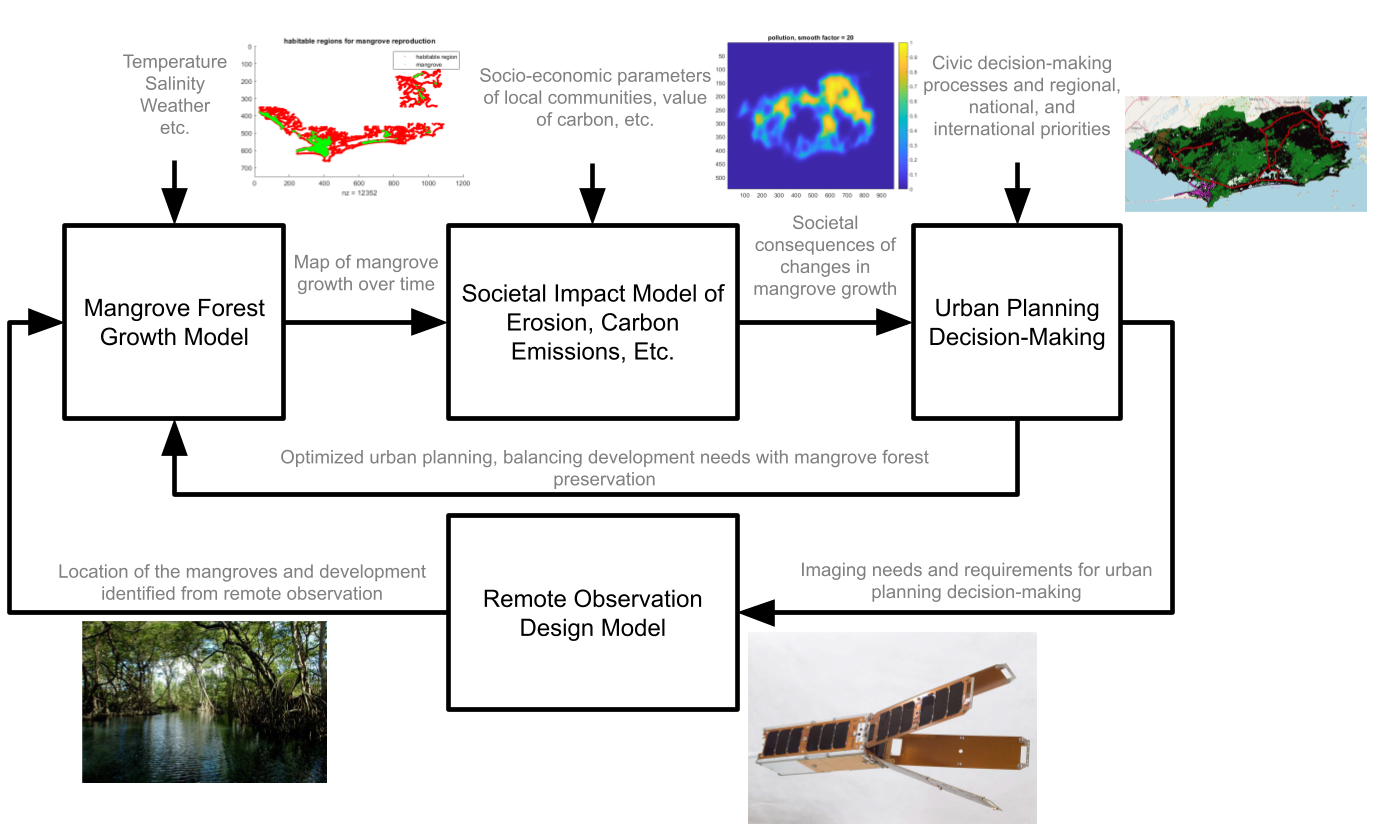
\includegraphics[width=0.9\textwidth]{Figures/chap4/MangroveModelFlow.png}
\caption[EVDT Model (Rio de Janeiro Mangrove Forest Case)]{Environment - Vulnerability - Decision - Technology Model (Rio de Janeiro Mangrove Forest Case)}
\label{fig:rio-evdt-flow}
\end{figure}


\subsection{\hlc[cyan]{EVDT Methodology}} \label{sec:rio-evdt-method}

\subsubsection{\hlc[cyan]{Environment}} \label{sec:rio-evdt-e-method}

The Environment Model of this case study is primarily interested in the the size (as measured by geographic extent) and health mangrove forest over time. Secondarily it is interested in the carbon stock and annual carbon export potential that they represent. Each of these are dependent of a variety of sources of data measuring and mapping mangroves.

Unlike some other forms of natural resources, which were extensively surveyed and quantified by colonial conquerors and explorers, historical information on pre-industrial Mangrove forest cover tends to be vague, primarily characterizing Mangroves as barriers to settlement \cite{amadorBaiaGuanabaraOcupacao2013}, likely due to historical perceptions of mangroves by colonists, who, as opposed to native inhabitants of the Americas, tended to view mangroves as gloomy sources of disease rather than as natural resources to be exploited \cite{friessEcosystemServicesDisservices2016}. Retroactive understanding of Rio de Janeiro area mangrove cover in this era has been supplemented by palaeoecological studies \cite{vilelaLateHoloceneEvolution2014} but only in a highly incomplete manner. 

This disregard for mangrove forests largely continued until, after a UN-led effort in the 1980s, international concern over their degradation increased, leading to greater efforts to monitor mangroves. In the second half of the 20th century, mangrove mapping efforts relied primarily on a combination of in-situ surveys and aerial and satellite photography. Investigations were typically site-specific, relied on human interpretation of images, and commonly only had one measurement every 1-2 decades \cite{lacerdaluizandmenezesmarceloandmussimolisanimauricioChangesMangroveExtension2007, fromardHalfCenturyDynamic2004}. These factors limited both spatial scalability and the potential for timely forest management. 


In the past decade, significant progress has been made to address these limitations by creating spatially explicit global mangrove forest cover, loss, drivers of loss, and carbon sequestration maps \cite{spaldingWorldAtlasMangroves2010, donatoMangrovesMostCarbonrich2011, sandermanGlobalMapMangrove2018, simardMangroveCanopyHeight2019, goldbergGlobalDeclinesHuman2020}. Due to both new remote observation datasets and novel analysis techniques,   spatial and temporal accuracy and resolution have significantly increased. The first global mangrove extent map with a consistent methodology and a spatial resolution of <1km was published in 2011 by Giri et al. using data from the Landsat series of \acp{eos} processed by hybrid supervised and unsupervised classification techniques \cite{giriStatusDistributionMangrove2011}. This map represented mangrove forest cover in the year 2000 specifically. 

More recently, the \ac{gmw} published an extent map with an improved classification methodology covering the years 1996, 2007, 2008, 2009, 2010, 2015, and 2016 \cite{buntingGlobalMangroveWatch2018}. This was accomplished by combining \ac{sar} data from the \ac{alos} \ac{palsar} platform with the Landsat data used by Giri et al. In 2010, the \ac{icesat} with its \ac{glas} was launched. The lidar data generated, when combined with the radar interferometry data from the \ac{srtm} in 2000, has similarly enabled the creation of global mangrove height maps \cite{simardMangroveCanopyHeight2019}, improving carbon storage estimates. 

Similar advances, often driven by improvements in machine learning, have yielded global maps of human land use, which can be combined with mangrove-related data products to accurately identify drivers of loss \cite{goldbergGlobalDeclinesHuman2020}. Most recently, these tools have been used to generate global datasets in which the specific years of degradation and regrowth are mapped \cite{vancutsemLongterm199020192021}.

Of these numerous sources of data and derived information, a subset were used to assess the Guaratiba region mangroves from the year 2000 to 2018. These data sources, along with what purpose they were put to are summarized in Table \ref{tab:rio-environment-sources}.

\begin{table}[!htb]
\caption[Datasets used for Rio Environmental Analyses]{Datasets used for each component of the environmental analyses performed for this case study}
\label{tab:rio-environment-sources}
\begin{center}
\scriptsize
\begin{tabular}{| C{3cm} |  C{2cm} | C{2cm} | C{2cm} | C{2cm} | C{2cm} |} \hline
 
\textbf{Data Source} & \textbf{Full Year Data Availability} & \textbf{Extent}  & \textbf{Health} & \textbf{Carbon} & \textbf{Reference(s)} \\ \hlinewd{2pt}

Landsat 5 \ac{tm} Collection 2 Surface Reflectance & 1984 - 2012 & \textbf{$\times$} & \textbf{$\times$} & & \\ \hline

Landsat 7 \ac{etm} Collection 2 Surface Reflectance & 1999 - 2022 & \textbf{$\times$} & \textbf{$\times$} & & \\ \hline

Landsat 8 \ac{oli} Collection 2 Surface Reflectance & 2013 - 2022 & \textbf{$\times$} & \textbf{$\times$} & & \\ \hline

\ac{alos} \ac{palsar}/\ac{palsar}-2 Yearly Mosaic & 2007 - 2010, 2015 - 2020 & \textbf{$\times$} &  & & \cite{shimadaNewGlobalForest2014} \\ \hline

Sentinel-2 \ac{msi} Harmonized Surface Reflectance & 2018 - 2022 & \textbf{$\times$} &  & & \\ \hline

Giri et al.'s Global Mangrove Forests Distribution, v1 & 2000 & \textbf{$\times$} &  & & \cite{giriStatusDistributionMangrove2011} \\ \hline

\ac{gmw} V2 & 1996, 2007 - 2010, 2015 - 2016 & \textbf{$\times$} &  & & \cite{buntingGlobalMangroveWatch2018} \\ \hline

Simard et al.'s Canopy Height & 2000 & & & \textbf{$\times$} & \cite{simardMangroveCanopyHeight2019} \\ \hline

\end{tabular}
\end{center}
\end{table}

These various data sources were used in a multi-step process was used to assess the state of the mangroves, as seen in Figure \ref{fig:extent_method}, to track changes in extent, health, and biomass of the mangroves from 2000 to 2018. The following subsections provide more details about each of these components. Unless otherwise stated, all \ac{eo} imagery processing and analysis took place using \acf{gee}, prior to being exported for use as part of the \ac{dss} (See Section \ref{sec:rio-dss}). \ac{gee} is a free, cloud-based, geospatial programming platform that hosts free satellite imagery from a variety of sources. This platform obviates the need to download such imagery onto a computer for individual manual analysis.

\begin{landscape}
\begin{figure}[t]
	\centering
	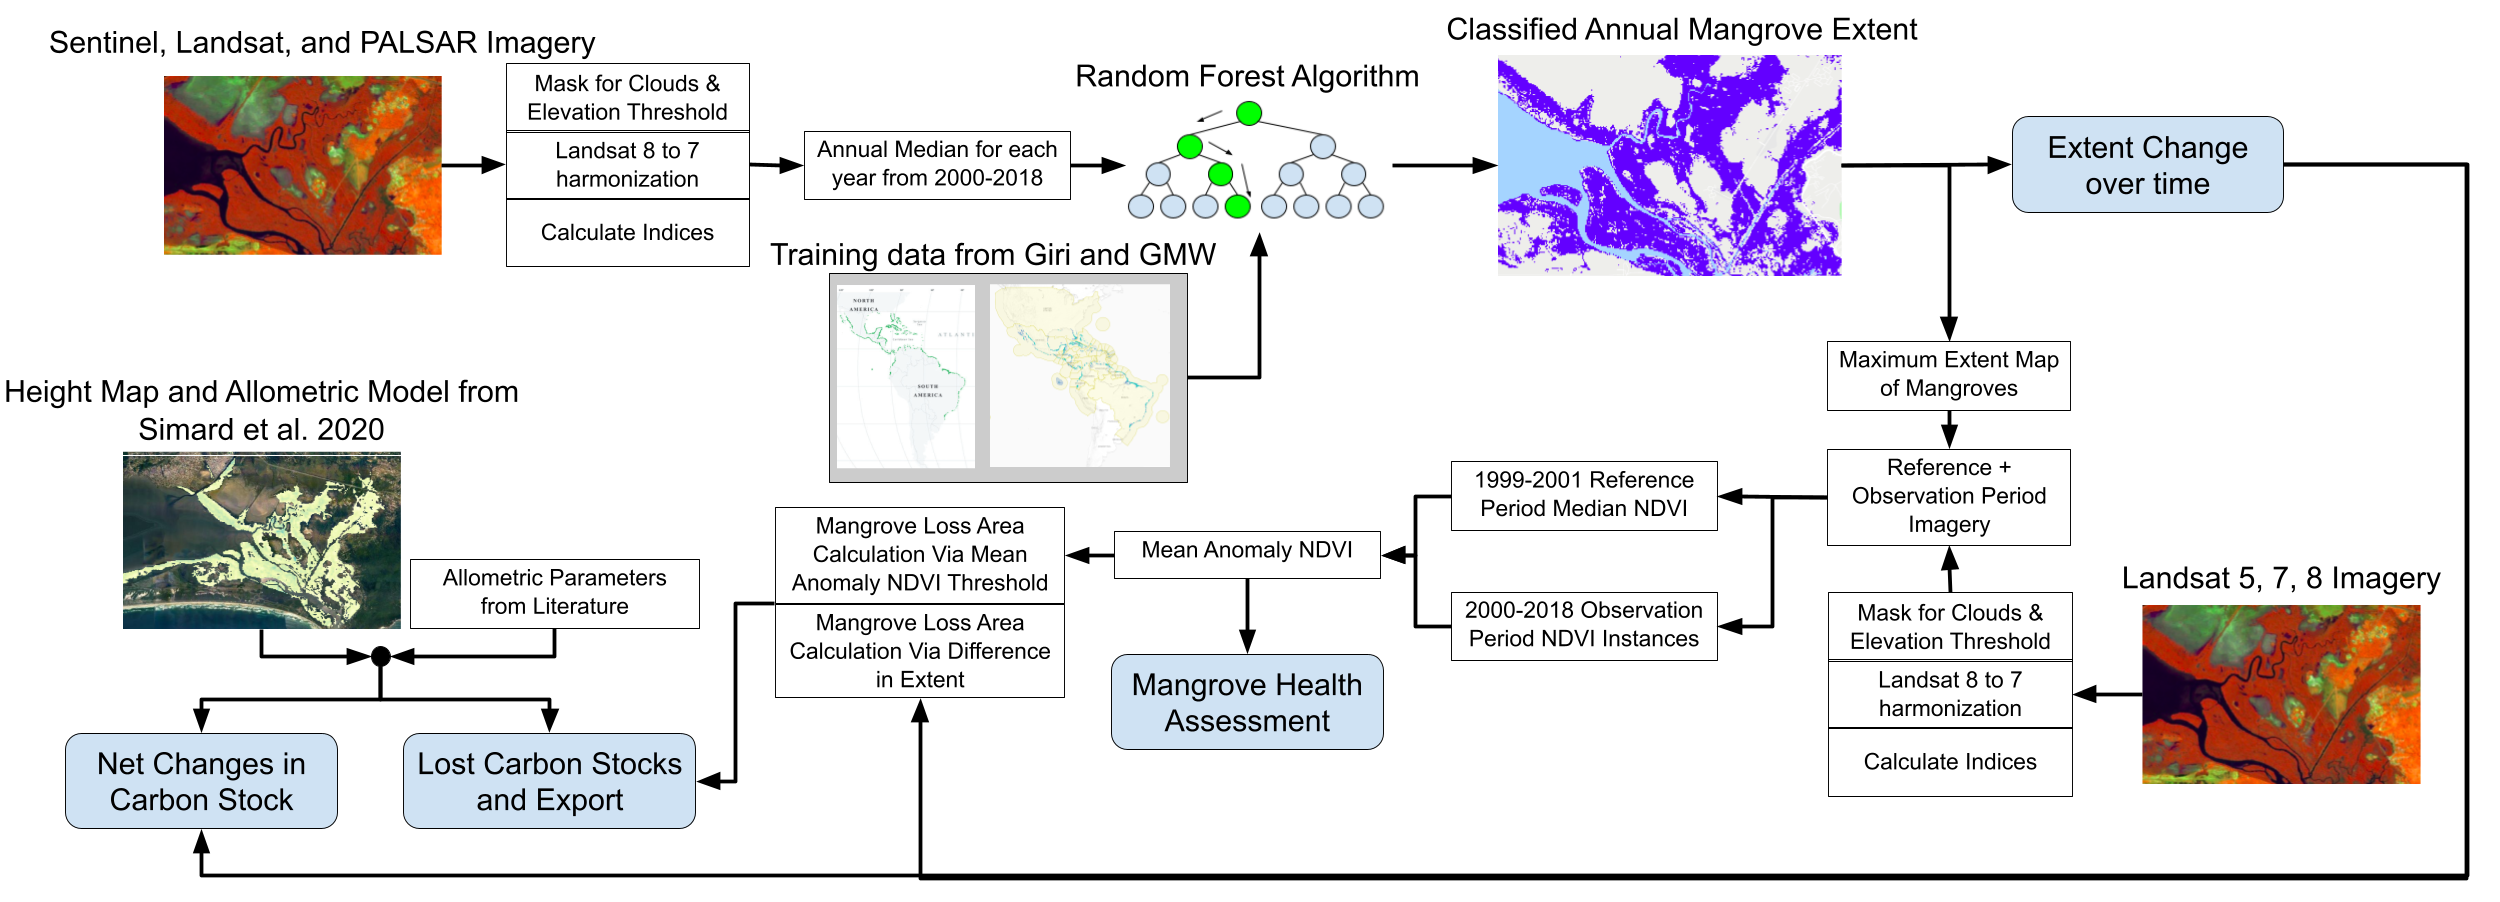
\includegraphics[scale=0.225]{Figures/chap4/extent_method.png}
	\caption[Mangrove Analysis Methodology]{Methodology for Analyzed Mangrove Extent, Health, and Carbon. Primary outputs are shown in blue boxes.}
	\label{fig:extent_method}
\end{figure}
\end{landscape}

\paragraph{\hlc[cyan]{Mangrove Extent}} \label{sec:rio-mangrove-extent} \leavevmode\newline

Regarding extent, the widely-used global mangrove extent maps such as Giri and \ac{gmw}, are typically representative of specific years and, due to their global-scale, often have higher errors in specific localities, particularly involving the landward edge of mangrove forests and smaller copses of trees. In order to conduct extent-change tracking and to identify such copses, it is sometimes preferred to conduct more targeted estimations, as was done in this case. Mangrove extent was estimated using a Random Forest Classifier (100 trees, 8 variables per split) utilizing both single-band surface reflectance imagery and several multi-band indices from Landsat 7 \ac{etm}, Landsat 8 \ac{oli}, Sentinel-2 \ac{msi}, and \ac{alos} \ac{palsar}. The indices used are summarized in Table \ref{tab:indices}. Not all of these satellites produced available data for the entire 2000-2018 range. For this reason, three separate versions of the classifier were trained, one that only uses Landsat data (full date change); one that uses Landsat and \ac{palsar} (for the years that \ac{palsar} data is available); and one that uses Landsat, \ac{palsar}, and Sentinel-2. Training data was identified using a combination of Giri's 2000 map, \ac{gmw}'s 2015 map, and firsthand field visits. 

In order to eliminate false positives, a mask was used to filter out flagged pixels at over 40m in elevation, as determined by the \ac{srtm} dataset \cite{jarvisHolefilledSRTMGlobe2008}. For a more detailed explanation of random forest classifier algorithms and their relevance to forest identification, see \cite{jhonnerieRandomForestClassification2015}.

For validation, the initial plan was to conduct \ac{uav} surveys of various parts of the Guaratiba mangrove forests. One such test survey for a particular plot of land was conducted in collaboration with the ESPAÇO research group in March of 2020. During the same visit, non-systematic visual inspection of areas identified by the classifier as damaged or lost mangroves were also conducted. The onset of the pandemic interrupted these plans, so instead validation relies upon comparison across the three classifiers, and with the Giri and \ac{gmw} maps.

Planet Lab's PlanetScope surface reflectance imagery was also experimented with, but ultimately was determined to not provide sufficient identification improvements to warrant continued use. 

Once the mangrove extent for each year has been classified, changes in extent can be identified for future consideration. Additionally an "all years inclusive" extent map can be generated, providing a basis for the spatial area to monitor for changes in vegetation health. 


\begin{table}[H]
\caption[Indices Used For Mangrove Classification]{Indices used for mangrove classification. Each of these were computed for both the Landsat and Sentinel-2 imagery. $R$ refers to surface reflectance values, with the subscripts indicating the specific band of light.}
\label{tab:indices}
\begin{center}
\scriptsize
\begin{tabular}{| C{2.5cm} |  L{4.5cm} | C{2.5cm} | C{2cm} |} \hline

 
\textbf{Index} & \centering \textbf{Description} & \textbf{Equation} & \textbf{Reference(s)}  \\ \hlinewd{2pt}

\ac{ndvi} & Popular index used to identify vegetation and monitor changes in vegetation health & $\frac{R_{NIR} - R_{red}}{R_{NIR} + R_{red}}$ & \cite{fredenMonitoringVegetationSystems1974,haboudaneHyperspectralVegetationIndices2004, pettorelliUsingSatellitederivedNDVI2005} \\ \hline

\ac{ndmi} & Used to distinguish mangroves from terrestrial forests & $\frac{R_{SWIR2} - R{green}}{R_{SWIR2} + R_{green}}$ & \cite{shiNewSpectralMetrics2016} \\ \hline

\ac{mndwi} & Used to identify water, particularly in areas with significant vegetation, soil, and built-up noise. & $\frac{R_{green} - R_{SWIR1}}{R_{green} + R_{SWIR1}}$ & \cite{xuModificationNormalisedDifference2006} \\ \hline

\ac{sr} & An old and popular index used to identify vegetation and monitor changes in vegetation health & $\frac{R_{NIR}}{R_{red}}$ & \cite{jordanDerivationLeafAreaIndex1969} \\ \hline

Band Ratio 54 & Used to monitor soil moisture & $\frac{R_{SWIR1}}{R_{NIR}}$ & \cite{ngothiEffectiveBandRatio2019} \\ \hline

Band Ratio 35 & Extension of the \ac{sr} concept to examine vegetation moisture & $\frac{R_{Red}}{R_{SWIR1}}$ & \cite{jiTerminologySpectralVegetation2011} \\ \hline

\ac{gcvi} & Used to monitor the content of leaf chlorophyll in vegetation and thus indirectly to monitor plant stress $ frac{R_{NIR}}{R_{green}}-1$ & \\ \hline

\end{tabular}
\end{center}
\end{table}


\paragraph{\hlc[cyan]{Mangrove Health}} \label{sec:rio-mangrove-health} \leavevmode\newline

While the classifier seeks to identify what land contains mangroves, it does not provide any information regarding the current or past health of those mangroves. For that we must turn to other approaches. Ultimately we elected to use the relatively simple and robust \ac{ndvi}, a normalized difference ratio of \ac{nir} and red surface reflectance, as seen in Table \ref{tab:indices}. \ac{ndvi} returns a value between -1 and 1, with 1 indicating a high likelihood of healthy vegetation, -1 indicating an absence of vegetation, and intermediate values indicating either possible vegetation or unhealthy vegetation, as seen in Figure \ref{fig:gndvi}. In Landsat 8's \ac{oli}, the one of the instruments used for tracking \ac{ndvi} in this case study, the \ac{nir} band captures \SIrange{0.845}{0.885}{\micro\metre} light while the red band captures \SIrange{0.630}{0.680}{\micro\metre} light. Landsat 5 and 7 surface reflectance imagery were used as well, harmonized according to Roy et al. \cite{royCharacterizationLandsat7Landsat82016}. \ac{ndvi} is the most commonly used surface reflectance index for tracking vegetation presence and health via remote observation, as well as being one of the more commonly used \ac{eo} indices overall \cite{fredenMonitoringVegetationSystems1974,haboudaneHyperspectralVegetationIndices2004, pettorelliUsingSatellitederivedNDVI2005}. 

\begin{figure}[H] 
\centering
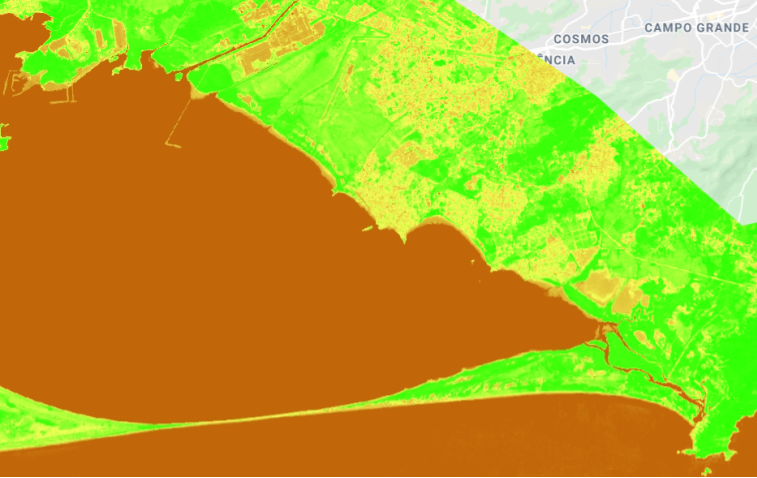
\includegraphics[width=0.49\textwidth]{Figures/chap4/guaratiba_ndvi.png}
\caption[False-Color image of area of interest showing an NDVI composite]{False-Color image of area of interest showing an NDVI composite. The greenest pixels indicate healthy vegetation presence}
\label{fig:gndvi}
\end{figure}

The specific metric used to assess mangrove health trends was \ac{ndvi} mean anomaly. The equation for this can be seen in equation \ref{eq:mean}. Here \textit{NDVI\textsubscript{Ref}} refers to the median \ac{ndvi} value at a specific location (an individual pixel in this case) over a specified reference period. \textit{NDVI\textsubscript{i}} refers to the \ac{ndvi} value at that location for each of the images taken during the observation period, and \textit{n} refers to the number of usable images (i.e. clear, no clouds, etc.) at a specific location. This metric has two primary benefits. First, it allows for a spatial consideration of health trends, where a straightforward \ac{ndvi} time series would show trends for only specific points or statistical aggregations. Second, unlike a mere start-end delta, the mean anomaly primarily represents significant, secular changes in mangrove health rather than cyclical or temporary changes. Both this method of health tracking and the classifier method of extent tracking is largely based upon methods used by Lagomasino et al. \cite{lagomasinoMeasuringMangroveCarbon2019, goldbergGlobalDeclinesHuman2020}.

\begin{equation}
\label{eq:mean}
Anomaly = \frac{\sum_{i=0}^{n} (NDVI_i - NDVI_{Ref})}{n}
\end{equation}

For this analysis, a reference period was defined as January 1st, 1999 to December 31, 2001 and the observation period was defined as January 1st, 2000 to December 31, 2018. It should be noted that mean anomaly is sensitive to the selection and duration of these periods, so the presented figures alone should not be taken as indicative of trends outside of the specified periods. 

\begin{figure}[H] 
\centering
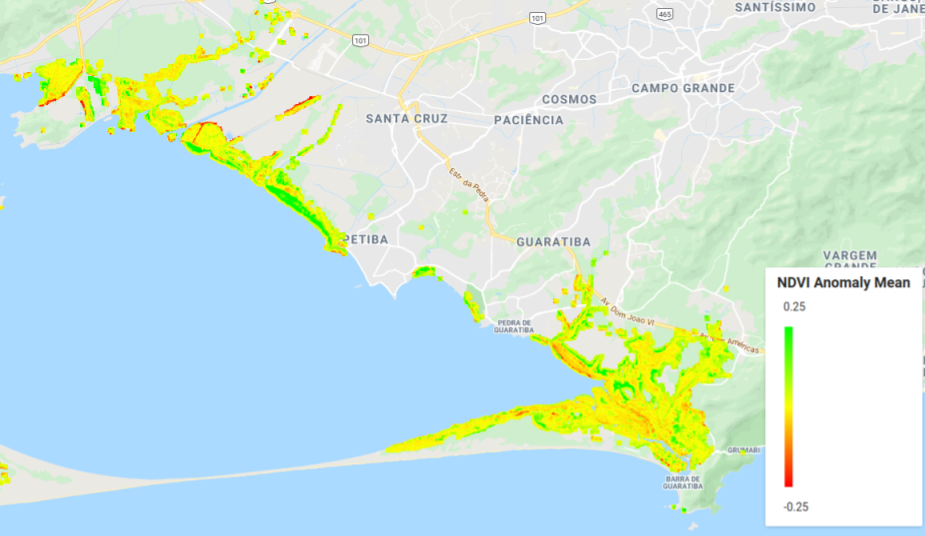
\includegraphics[width=0.49\textwidth]{Figures/chap4/guaratiba_anomaly.png}
\caption[False-Color image depicting NDVI mean anomaly]{False-Color image depicting NDVI mean anomaly. Green indicates new or healthier mangroves, red indicates reduction in extent or in health, yellow indicates no measured change.}
\label{fig:anomaly}
\end{figure}

\paragraph{\hlc[cyan]{Mangrove Height}} \label{sec:rio-mangrove-height} \leavevmode\newline

Previous I mentioned the Simard et al. 2020 global mangrove canopy height map was to be used in this analysis (see Table \ref{tab:rio-environment-sources}. While this map is specifically intended to represent the height of mangroves in the year 2000, it remains the best available information on mangrove height in the region. This however may not remain the case for long (see Section \ref{sec:rio-discussion} for discussion of ongoing data collection activities).

\paragraph{\hlc[cyan]{Mangrove Carbon Stocks and Exports}} \label{sec:rio-mangrove-carbon} \leavevmode\newline

Th height estimates from Simard et al. can be used to estimate \ac{agb} \cite{cloughAllometricRelationshipsEstimating1989, fatoyinboEstimatingMangroveAboveground2018, simardMangroveCanopyHeight2019}, which is important for improving estimates of the forests' carbon sequestration capabilities \cite{lagomasinoMeasuringMangroveCarbon2019}. 

To estimate \ac{agb} density for the Guaratiba area, I used the Americas generic power allometric model developed by Simard et al. \cite{simardMangroveCanopyHeight2019}, shown in Equation \ref{eq:allo} where $H_{ba}$ refers to the basal area weighted height of the mangroves. This equation was chosen as it contained the highest $R^2$ value (0.71) and lowest \ac{rmse} (54.3 MgC/ha) of the equations that cover the region. 

\begin{equation}
\label{eq:allo}
\ac{agb}_{density} = 1.418 * H_{ba}^{1.6038}
\end{equation}

By combining the Simard canopy height data with the Landsat-only extent classification\footnote{For mangroves identified by the Landsat-only extent classification that were not included in the Simard dataset, I assumed that $H_{ba}$ was equal to the average for the region.}, the \ac{agb} distribution of the region can be mapped for specific years.

To account for soil carbon and root biomass, in addition to \ac{agb}, Equation \ref{eq:carbon} was used. In it, $270.1$ represents an estimate of the mangrove soil carbon density in MgC/ha. This is based on 19 samples (which ranged from 135 to 376 MgC/ha) taken by Jennerjahn et al. 2002 \cite{jennerjahnRelevanceMangrovesProduction2002} in Sepetiba bay (as reported in \cite{kristensenOrganicCarbonDynamics2008, atwoodGlobalPatternsMangrove2017}), making it directly relevant to this case study.  Total root biomass was estimated at 49\% of the \ac{agb}, as is specified by \ac{ipcc} guidelines \cite{takahiko2013Supplement20062014} (thus the 1.49 multiplicative constant in Equation \ref{eq:carbon}). This accounting process is modeled after the methodology used in Simard et al. \cite{simardMangroveCanopyHeight2019}.

\begin{equation}
\label{eq:carbon}
C_{density} = 1.49 * \ac{agb}_{density} + 270.1 
\end{equation}

For annual rate of carbon export, I used 5.85 MgC/ha. This is based on two sources. The first is Estrada \cite{estrada2013analise} who sampled sites throughout the \ac{rbag}, sorted the mangroves into three categories, and estimated rate of \ac{agb} change resulting from growth and recruitment. These three categories are fringe, basin, and transition, for each Estrada estimated annual carbon sequestration rates of 2.64, 1.90, and 2.39 MgC/ha respectively. We can use these to calculate an area-weighted average of 2.05 MgC/ha-year. 

The other source is Lacerda \cite{lacerda1992carbon} (as reported in \cite{jennerjahnRelevanceMangrovesProduction2002}) who, based on samples liter fall from mangroves along the coast of Sepetiba bay, estimated an annual carbon sequestration rate of 3.8 MgC/ha (2.2 being exported into the ocean and the remainder being incorporated into the sediment).

Since these two sources both based on samples from the study area (albeit not in the precise same location) and they measure different mechanisms of carbon sequestration, I added them together to reach the figure of 5.85 MgC/ha-year. This is acknowledged to be imprecise both due to variations in the type of mangrove forest throughout the region and in the high levels of uncertainty in each of the underlying sources.

\subsubsection{\hlc[cyan]{Vulnerability}} \label{sec:rio-vulnerability}

Social impact and vulnerability in this case study has several different forms. First there are general socioeconomic trends and pressures in the Guaratiba area. Secondly, there are the ecosystem services provided, directly or directly, by the mangroves. Ecosystem services are often sorted into three categories: provisioning (providing some raw material), regulating (moderating the ambient environment in a helpful manner), and cultural (non-material benefits) \cite{haines-youngCommonInternationalClassification2018}. Mangrove forests around the world provide each of these:

\begin{itemize}[itemsep=0pt,parsep=0pt]
	\item{Provisioning: Fuelwood / timber}
	\item{Regulating: Water filtration, protection from coastal erosion and storms\footnote{Some studies place protection from coastal erosion and storms into a fourth category, supporting/maintaining, rather than in regulating \cite{getznerEcosystemServicesMangrove2020}.}, hosting fisheries}
	\item{Cultural: Tourism, general biodiversity}
\end{itemize}

The following subsections detail the data and methods used to approach both the general socioeconomic condition of the inhabitants of the study area and the ecosystem services provided by the mangroves. For the latter, I further separate out the carbon regulating services from all other such services.

\paragraph{\hlc[cyan]{Socioeconomic Situation}} \leavevmode\newline

A qualitative history of these was presented in Section \ref{sec:rio-context}. In addition to this history, various quantitative socioeconomic and demographic data, including employment rates and population density, were collected at several geographic scales, including bairros (neighborhoods), census blocks, and census microgrids. Much of this data was sourced from the national statistics agency, the \ac{ibge}. These were supplemented with municipally collected data, organized by \ac{ipp}. Such data includes a UN-developed \ac{ipm} \cite{oxfordpovertyandhumandevelopmentinitiativeChartingPathewaysOut2020}, a municipally-customized \ac{ips} \cite{puliciRelatorioMetodologicoIndice2016}, and detailed land use / land cover maps \cite{regoAutomaticClassificationLand2003}. In particular I relied upon 2016 employment sector data \cite{institutopereirapassosNumeroEmpregadosPor2018} and 2010 population data \cite{institutopereirapassosPopulacaoResidentePor2018}.

This data varies significantly in its geographic and temporal resolution. This process was primarily descriptive and provided the basis for various layers to be displayed in the \ac{dss}.

\paragraph{\hlc[cyan]{Carbon Regulation Ecosystem Services}} \leavevmode\newline

When it comes to mangrove ecosystem services, we can separate out carbon regulating as these have already been estimated in the Environment section of this chapter. All that remains is to put a value on those amounts and rates of carbon.

One option is to use a government-endorsed price that is actively traded on a market. In 2017, Brazil created the RenovaBio program which sells carbon credits, called CBIOs, in exchange for biofuel production. Using CBIO prices pose two problems. First is that CBIO prices have been highly variable, ranging from 10USD/MgC \cite{castroBrazilianCarbonCredit2020} to more than 38USD/MgC \cite{barrosBiofuelsAnnual2022}. This is compounded by the fact that CBIOs were first sold in 2020, after the period of study, preventing us from directly linking annual carbon sequestration with a particular CBIO price for that year.

The other problem with using CBIO prices is that they are intended to encourage biofuel production and are not necessarily representative of the actual value of carbon in general or of mangrove forests in particular.   

This can be compared to estimates for specifically the Guaratiba reserve (as opposed to the full region) by Estrada et al. They estimated that the Guaratiba mangrove forest, as of the year  sequester approximately \$456K of worth of carbon per year and their total \ac{agb} represents \$3.5M \cite{estradaEconomicEvaluationCarbon2015}. It should be noted that they used a somewhat different methodology, first estimating the extent of different types of mangrove forest within the reserve (fringe, basin, transition) and the typical carbon storage/sequestration levels for each of these types. These were then multiplied by a value of \$18/MgC, attributed to Medeiros et al. \cite{medeirosContribuicaoUnidadesConservacao2011}. 

Confusingly enough, Medeiros et al. does not contain this valuation nor do they create their own valuation. Instead, they refer to Hamilton et al. \cite{hamiltonStateForestCarbon2010} to pull the value of \$4.76/MgC. Estrada et al. meanwhile separate cites Hamilton et al. for a figure of \$7.88/MgC. Upon examining Hamilton et al. myself, it appears that they conducted a global survey of EU forest carbon credits in 2009. \$7.88/MgC was the volume-weighted average price that they found. \$4.76/MgC was the average of EU \ac{tcer} credits, which must be replaced or reissued at the end of their crediting period (which is the end of the commitment period of the Kyoto Protocol following the one in which they were issued) \cite{salinasNonpermanence2011}. Notably, neither Estrada nor Medeiros updated this dollar amounts from 2009 to the years in which their studies took place. 

Using EU carbon credits such as \acp{tcer} is not without its flaws either. These credits are fundamentally tied to specific emissions-reduction projects and not intended to measure non-project-related carbon stocks and sequestration. They are also time-limited for variable amounts of time, making it difficult to directly calculate the net present value of a forest in its entirety \cite{salinasNonpermanence2011}. Finally their price has fluctuated significantly. Since their creation in 2005 to 2018, they have varied from a minimum of around 0.10USD/MgC in the summer of 2007 to a peak of around 40.28USD/MgC in June of 2008. More recently, over the course of 2018, the price steadily increased from 10.96USD/MgC to 29.54USD/MgC (none of these values have been converted to the present year) \cite{EUCarbonPermits2023}. Ultimately, in keeping with the study period of 2000 to 2018, with the intent of supporting decisions around 2018, I elected with to conduct the valuation using the average 2018 EU carbon credit price of 19.46USD/MgC, acknowledging that prices would continue to fluctuate (overwhelming upwards) after this period. 

\paragraph{\hlc[cyan]{Non-Carbon Ecosystem Services}} \leavevmode\newline

As mentioned previously, it is known that the local communities in the Guaratiba area benefit from various ecosystem services provided by the mangroves, but the exact forms these services take are unknown and their values have not been quantified. Some bounds on these values can be estimated from valuation studies focusing on mangroves elsewhere in the region and elsewhere around the world. Prof. Suyhun Jung, Emily Joiner, and I examined mangrove ecosystem services valuations from the \ac{esvd} \cite{grootEcosystemServicesValuation2020} (an open source database maintained by the Foundation for Sustainable Development) and nine meta-analyses or review papers \cite{branderEmpiricsWetlandValuation2006,branderEcosystemServiceValues2012, salemEconomicValueMangroves2012, veghMangroveEcosystemServices2014, voReviewValuationMethods2012, himes-cornellMangroveEcosystemService2018, getznerEcosystemServicesMangrove2020, barbierProtectiveServiceMangrove2016, barbierEstuarineCoastalEcosystems2020} as part of a broader project to developed a refined global range of mangrove ecosystem services \cite{jungGapsMangroveForestInReview}.

Even after curating these sources for methodological reliability and comparability (see \cite{jungGapsMangroveForestInReview} for more details), significant variation remained. Cultural/aesthetic value varied from \$0/ha to \$18K/ha (in international 2020 dollars) while one outlier on the value of food provisioning placed it's value at approximately \$65K/ha when others placed it at near zero. Focusing on just subsistence-related ecosystem services reduces but does not elimate such variance. Timber \& non-timber forest products were valued \$0/ha -\$1K/ha, capture fisheries between \$0/ha - \$2K/ha, and shoreline protection \$0/ha - \$5.5k/ha (though with two outliers around \$13K/ha).

Directly applying these ranges to the Guaratiba area would result in significant errors, however. The underlying studies are from around the world and involve very different societies, economies, and ecosystems. The studies taking place in Brazil not only constitutes a minority of such studies but in fact have been disproportionately few compared to the extent of mangroves in the country, as can be seen in Figure \ref{fig:mangrove_area_studies}. Within South America, Columbia has ~5 times as many studies despite having only around one quarter as many mangroves. Globally, the bulk of the studies have taken place in southern and south eastern Asia. 

\begin{figure}[!htb] 
\centering
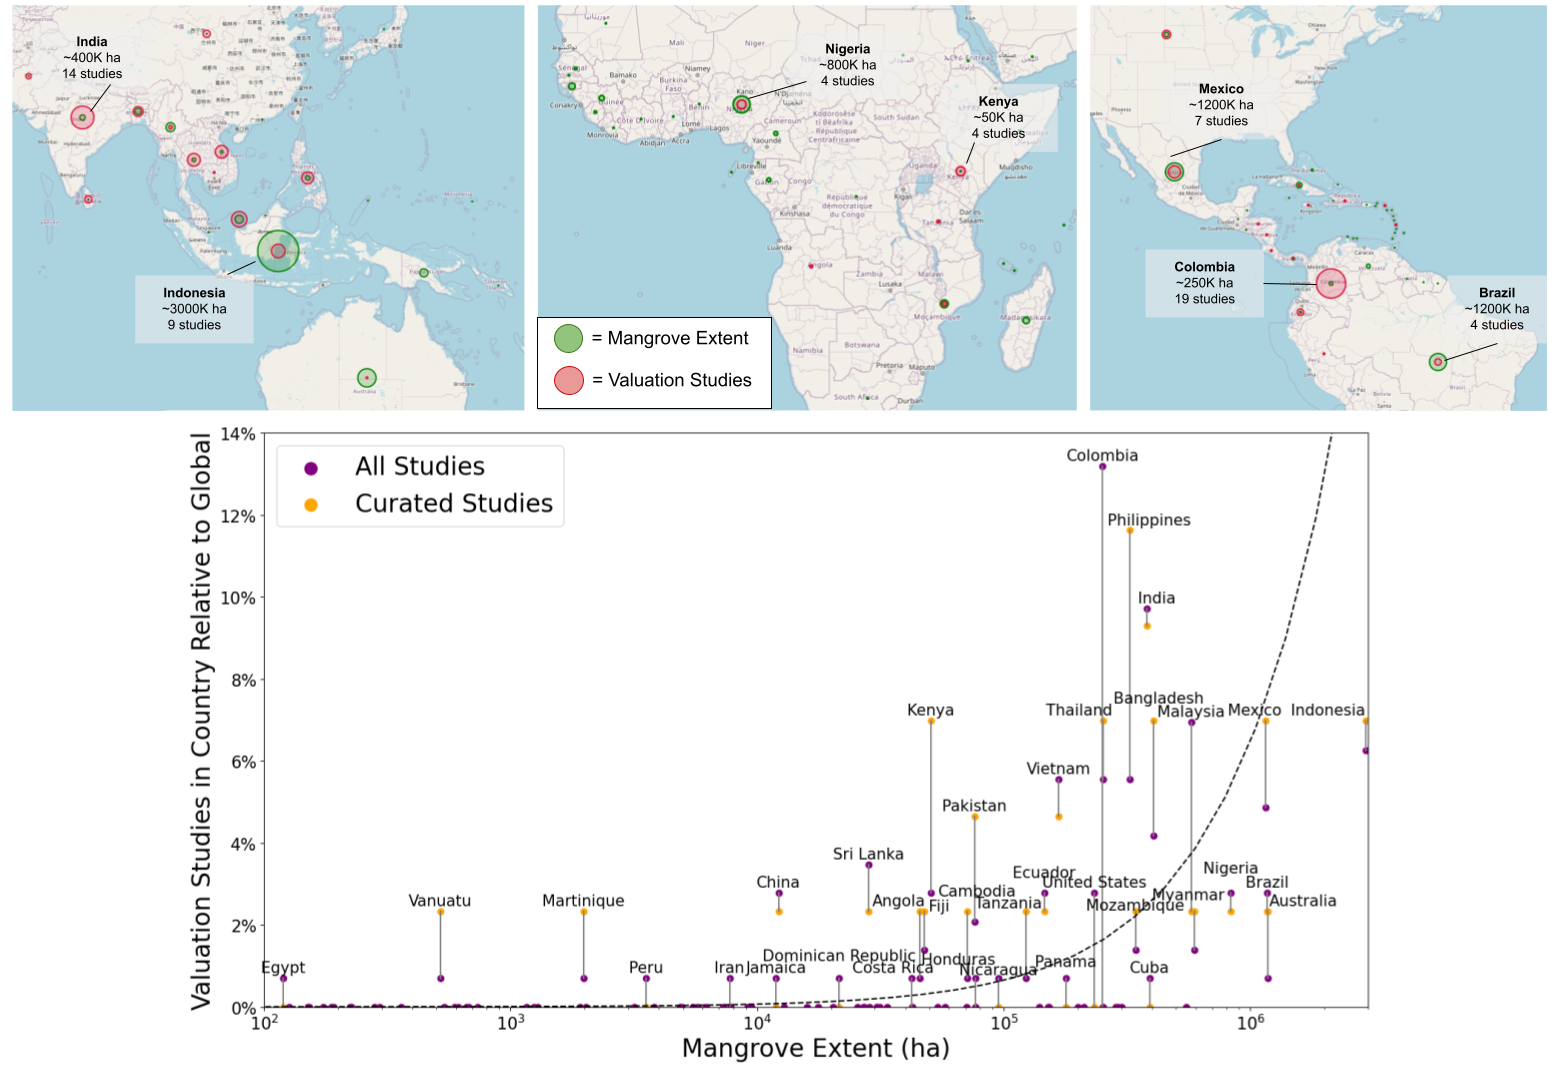
\includegraphics[width=0.95\textwidth]{Figures/chap4/mangrove_area_studies_graphic_combo.png}
\caption[Mangrove Valuation Studies Compared to Mangrove Extent]{Top: Maps comparing pre-curation mangrove valuation studies relative to mangrove areal extent by nation. Red and green circles of equal size indicate that the proportion of the valuation studies in that country compared to all studies matches the proportion of mangrove extent in that country compared to the global extent. E.g., Nigeria contains 3 percent of the studies and 5 percent of the global mangrove extent, so the circles are approximately the same size. India, however, contains 10 percent of the studies but only has 2 percent of the world’s mangroves, so the red circle is significantly larger than the green circle.
Bottom: A graph showing how the relative portions of studies taking place in each country compared with mangrove extent. The black dashed line indicates where the proportion of the valuation studies in that country compared to all studies matches the proportion of mangrove extent in that country compared to the global extent (comparable to red and green circles of the same size in the map).}
\label{fig:mangrove_area_studies}
\end{figure}

If we focus on the studies more particular for Brazil, we have Estrada et al. \cite{estradaEconomicEvaluationCarbon2015}, which focused on the local and was previously discussed with regards to carbon storage and valuation \ac{rbag}; de Rezende et al. \cite{derezendeEconomicValuationMangrove2015}, which studied the Pariaba do Sul River estuary in the northern portion of the state of Rio de Janeiro, approximately 300km to the northeast of this chapter's study area; and Souza \& Ramos e Silva \cite{souzaEcologicalEconomicValuation2011}, which studies the Potengi River estuary in northeastern Brazil, approximately 2100km from our study area.

The first of these only valued carbon and thus is not relevant to non-carbon ecosystem services.  The second used choice experiments to study preferences for mangrove restoration. This involved surveying individuals in the larger public plazas in cities near the mangrove forests of the estuary. This essentially seeks to approximate how much individuals would be filling to pay to preserve or restore the mangroves and then extrapolate that to the entire community (in this case, the state of Rio de Janeiro). It thus does not distinguish what types of ecosystem services are valued. de Rezende et al. ultimately come up with the range of \$21K/ha - \$380k/ha (or only \$0.4K/ha - \$7.5k/ha if only the willingness to pay of the communities closest to the mangroves are considered).

Souza \& Ramos e Silva meanwhile sought to estimate the value of tourism (using data from local transit and tourism operators); aquaculture (using local market prices and volumes); and water quality, specifically nitrogen phosphorus, and heavy metals (by determining the cost of an equivalent water treatment center). They come to an estimate of \$4K/ha for tourism, \$8.7K for aquaculture, and \$15.5K/ha for water treatment. While they do not specify what year these dollar amounts are for, it appears that the bulk of their research took place in 2009. Converting these to 2018 dollars results in \$4.5K/ha, \$9.7K/ha, and \$17.3K/ha, respectively.

I rely upon the estimates from this last source primarily, as despite the study taking place in another part of the country, they represent the primary non-carbon ecosystem services of concern in the Guaratiba area while also being well within the range of values noted in the broader metastudy \cite{jungGapsMangroveForestInReview}. 

\subsubsection{\hlc[cyan]{Decision-making}}

Two primary policy decisions are currently included in this \ac{evdt} application: conservation status and urban zoning. The histories of these are provided by the municipal Environmental Secretariat and Urban Planning Secretariat and accessed via the Data.Rio platform. The urban zoning categories are broadly similar to those in many cities around the world and include the types of commercial and industrial activity permitted and maximum floor area ratio allowed, among other factors. 

Conservation status, on the other hand, is more complicated, as discussed in Section \ref{sec:rio-jurisdictions}. Some of these protected areas are classed as ``integral protection," meaning little or no development and resource extraction is allowed. In addition to these areas (and often surrounding them), there are various municipally-defined ``sustainable use" areas that allow for certain, restricted forms of development and resource extraction. There are also two different classes of ``boundary zones" with yet fewer protections.

The selection of these two axes of policy decisions (conservation status and urban zoning) was based on meetings and discussions with government officials from several municipal and federal agencies, university researchers, and local community members. Other axes were discussed and were of interest to particular audiences (such as transit network changes, conservation policy enforcement stringency, and sewage infrastructure improvements), but these two held broad appeal and relative accessibility, while still having concrete historical data that are either quantitative or code-able qualitative in nature. 

For each of these two axes, I sorted protected areas and zones into various categories. For each of these categories, I calculated both the absolute extent of mangroves loss during the 2000 to 2018 period and the relative amount of mangrove loss, compared to the full extent of mangroves. Loss extent was determined by the \ac{ndvi} mean anomaly threshold from Section \ref{sec:rio-evdt-e-result}. This enabled us to see if there is any correlation between municipal government restrictions and mangrove losses.

\subsubsection{\hlc[cyan]{Technology}}

The primary technologies of interest in this project are sensing and measurement methods for informing policymakers and the other \ac{evdt} components. Among the commonly noted concerns during the stakeholder analysis process discussed in Section \ref{sec:rio-saf} were gaps in data on important topics, including changes in land cover, the value of ecosystem services, and the state of the environment. To better understand the current state of system, I inquired what sensing technologies or methods various stakeholders were currently using. The Technology component of this project will summarize this history of use and identify potential additional sensing technologies that may be of use. 

In the future, the \ac{evdt} Framework is intended to inform sensing technology selection and design. While this is not a major focus of this thesis or this case study, the potential for this will be discussed further in Section \ref{sec:rio-discussion}.

\subsection{\hlc[cyan]{EVDT Results}} \label{sec:rio-evdt-result}

\subsubsection{\hlc[cyan]{Environment}} \label{sec:rio-evdt-e-result}


\paragraph{\hlc[cyan]{Mangrove Extent}} \leavevmode\newline

We can see the differences, including both losses and new growth, of the mangroves between 2000 and 2018, as classified by the Landsat-only process, in Figure \ref{fig:extent-changes}. This represents a net increase of approximately 290 ha from 2000 to 2018, an approximately 9\% increase compared to the 3200 ha present in 2000.

The primary areas of new mangroves in Guaratiba proper (shown in blue on the right of Figure \ref{fig:extent-changes}) are along the interior gaps in the forests. This areas, called \textit{apicum} in Brazilian Portuguese, consist of a mix of sand and salt marshes, and are a natural part of the mangrove forest ecosystem. The mangroves commonly encircle these areas and generate soil in them prior to the trees themselves sprouting along their edges. The primary areas of lost extent (shown in red) occur along the human-forest interface and, to a less extent, along the water ways of the biological reserve. In the northwest corner of the right image (between Pedra de Guaratiba and Sepetiba) can be seen new growth in smaller protected areas immediately adjacent to built-up land.

In the left-hand image, different phenomena are apparent. The primary areas of new growth are along the coast, adjacent to Rio Guandu, a canalized river used as discharge by the Ternium steel plant and other industrial sites in Santa Cruz Industrial District. Primary losses meanwhile are directly along that, and the other canals, likely due to construction that took place around 2010. 
	
\begin{figure}[H] 
\centering
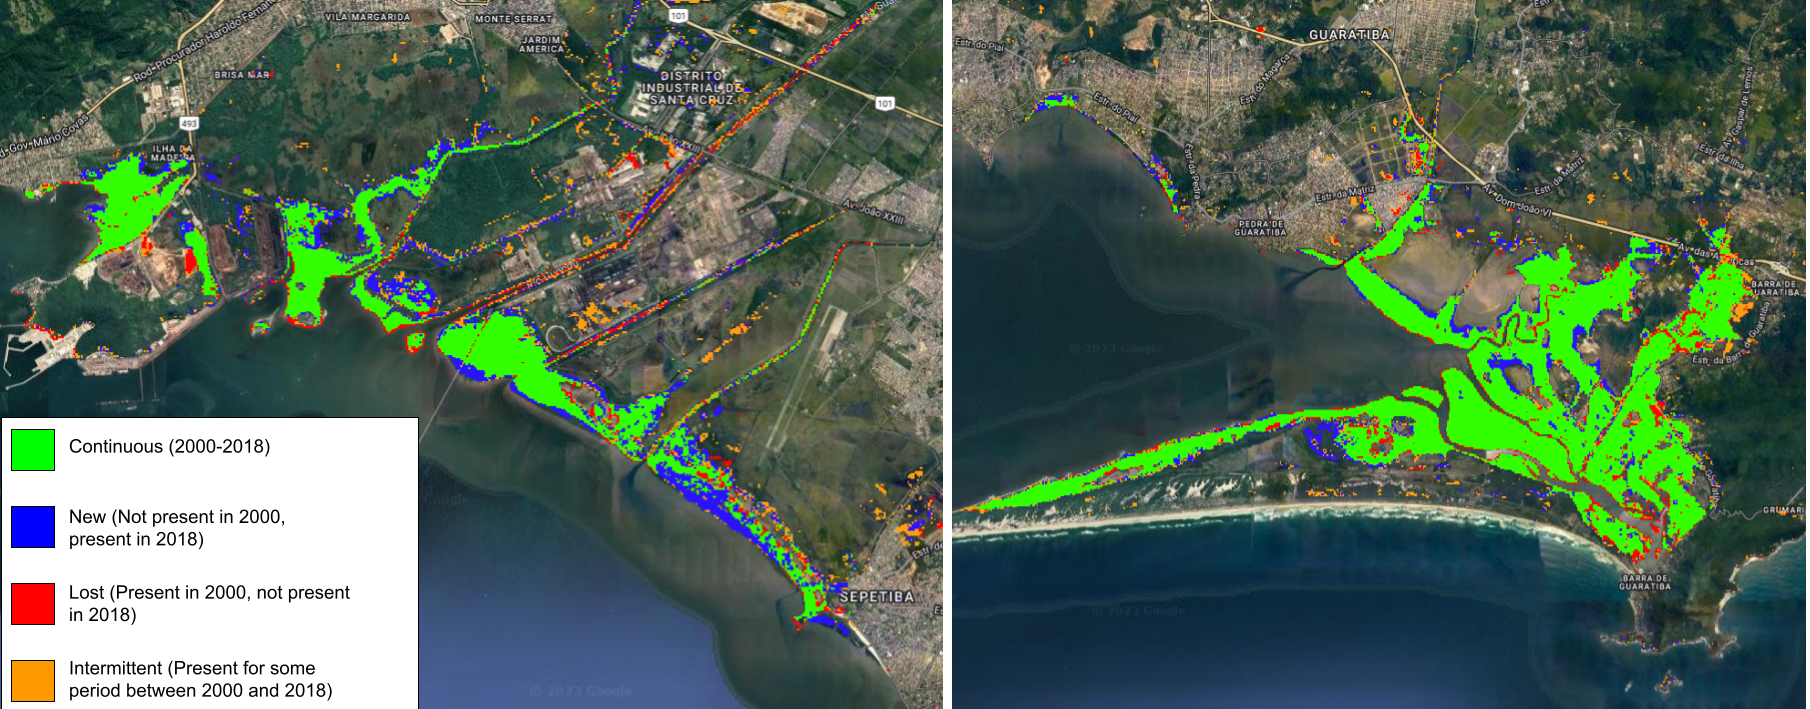
\includegraphics[width=0.95\textwidth]{Figures/chap4/extent_changes.png}
\caption[Changes in Mangrove Extent 2000-2018]{Changes in mangrove extent in western Rio de Janeiro from 2000 to 2018 as classified by the Landsat-only process. Left: Ilha da Madeira, Santa Cruz, and Sepetiba. Right: Guaratiba and Pedra de Guaratiba}
\label{fig:extent-changes}
\end{figure}

The net changes in extent can also be seen temporally rather than spatially in Figure \ref{fig:extent-over-time}. This graph also compares the three different classifier processes used, along with the Giri and \ac{gmw} maps. As is expected, both of the global maps provide lower estimates for mangrove extent. It is notable, however, that the \ac{gmw} maps indicate quite little changes over time, seeming to miss many of the local phenomena just discussed. That said, the estimates provided by the Landsat + \ac{palsar} classification suggest that the Landsat-only classification is somewhat overestimating mangrove extent. It does seem to confirm the general trend of  increasing extent from approximately 2005 to 2018, however.  

\begin{figure}[!htb] 
\centering
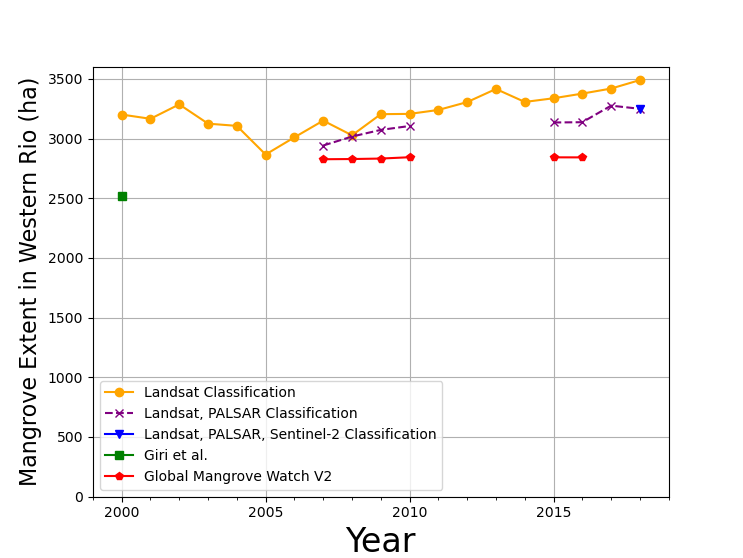
\includegraphics[width=0.95\textwidth]{Figures/chap4/extent_over_time.png}
\caption[Mangrove Extent Over Time]{Mangrove extent in western Rio de Janeiro from 2000 to 2018 as measured by several different classification methods.}
\label{fig:extent-over-time}
\end{figure}

The Landsat-only classifications for each year from 2000 to 2018 were used to construct an "all years inclusive" extent map that shows all areas that were classified as mangroves in at least one year. This was used as to identify the area for health tracking.

\paragraph{\hlc[cyan]{Mangrove Health}} \leavevmode\newline

We can see the median \ac{ndvi} values for the 1999-2001 reference period in Figure \ref{fig:reference_median}. As might be expected, the highest \ac{ndvi} values are present in the interior, mature ares of the forest, with lower \ac{ndvi} values lying along the edge. However, it cannot be determined from this image alone whether these lower value areas represent areas of new growth (young saplings in previously unoccupied land or water) or areas of degraded health / loss.  

\begin{figure}[!htb] 
\centering
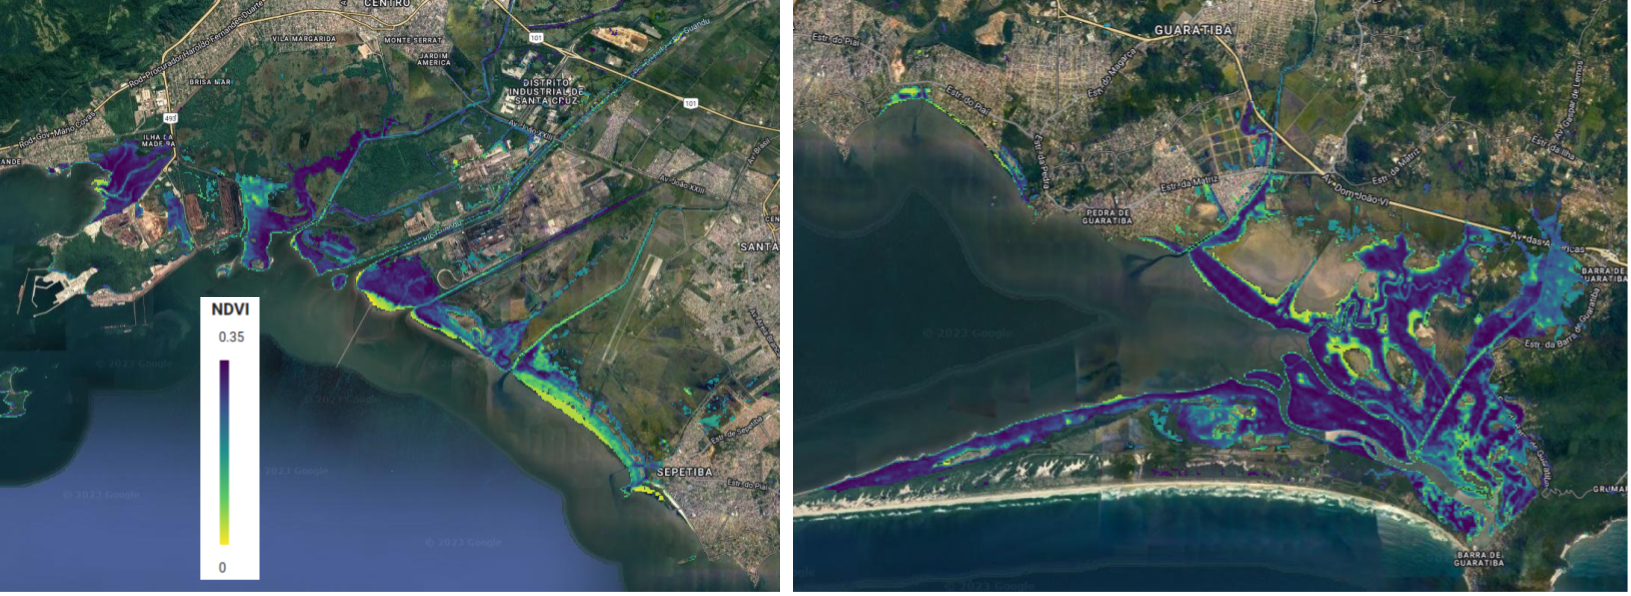
\includegraphics[width=0.95\textwidth]{Figures/chap4/reference_median.png}
\caption[Reference Median NDVI of Region]{Median NDVI for the reference period of 1999-01-01 through 2001-12-31. Left: Ilha da Madeira, Santa Cruz, and Sepetiba. Right: Guaratiba and Pedra de Guaratiba.}
\label{fig:reference_median}
\end{figure}

We can see the mean anomaly \ac{ndvi} in Figure \ref{fig:mean_anomaly_map}, which seems to corroborate the changes in classified extent presented in the previous section. In Guaratiba proper (in the right image), sustained increased in \ac{ndvi} are clearly evident along the interior apicum, while some (ambiguous) decreases are seen along the mangrove-human interface and the waterways. Similarly, in the left-hand image we can see the increases in \ac{ndvi} adjacent to the canal outlets and decreases along the canals themselves. In fact, it seems that, in addition to the noted increase in seaward extent noted previously, even the more interior mangroves downcurrent from the canal outlets have experienced significant growth. 

\begin{figure}[!htb] 
\centering
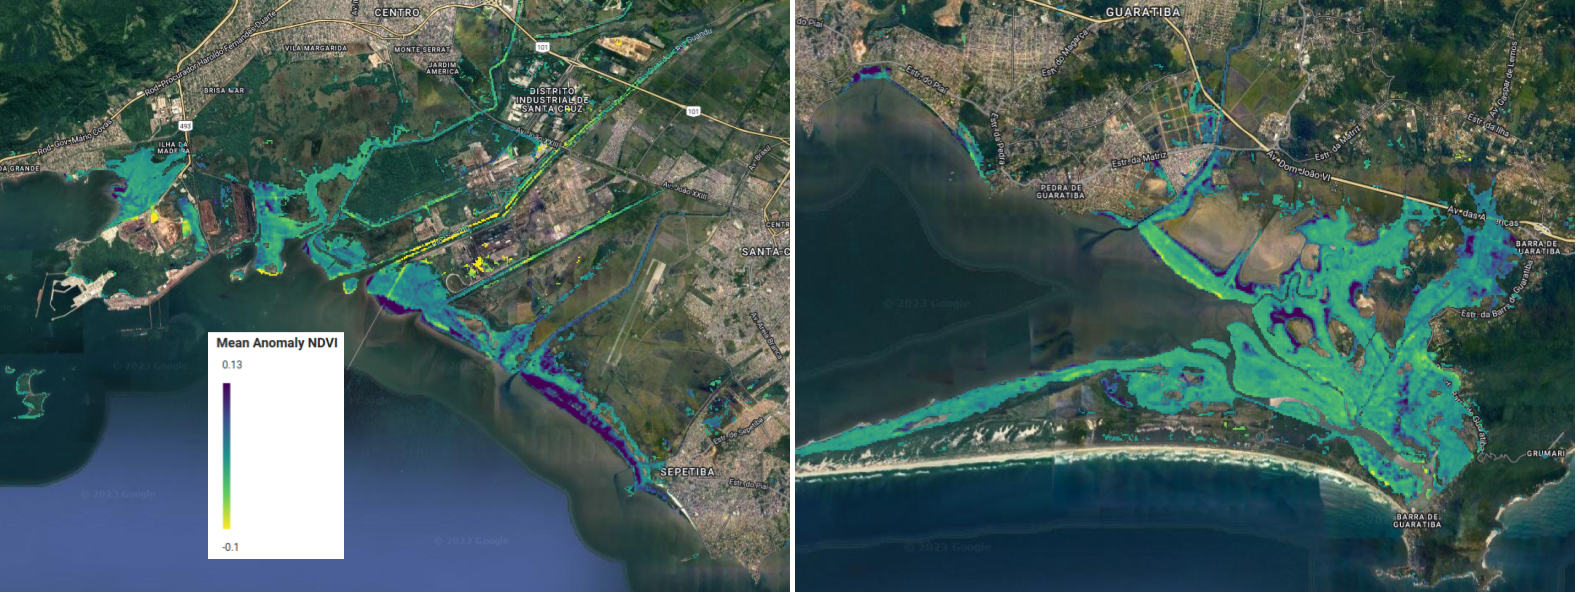
\includegraphics[width=0.95\textwidth]{Figures/chap4/mean_anomaly_map.png}
\caption[2000-2018 Mean Anomaly NDVI of Region]{2000-2018 Mean Anomaly \ac{ndvi}. Left: Ilha da Madeira, Santa Cruz, and Sepetiba. Right: Guaratiba and Pedra de Guaratiba.}
\label{fig:mean_anomaly_map}
\end{figure}

The areas of potential loss or damaged, as measured by changes in mean anomaly \ac{ndvi}, have been isolated in Figure \ref{fig:loss_map}, making the above noted changes more stark. In total these sum to approximately 108 ha of lost or damaged mangroves. In addition to the losses along the industrial canals, some loses can be seen in what is now the steel mill, representing its construction which began in the mid-2000s.  I visited many of the marked areas within the Guaratiba reserve (the right-hand image) during the August 2019 field visit and (non-systematically) confirmed that degradation was apparent in each of them, as can be seen in Figure \ref{fig:mangrove_photo}, though the causes of the degradation was not readily apparent.

\begin{figure}[!htb] 
\centering
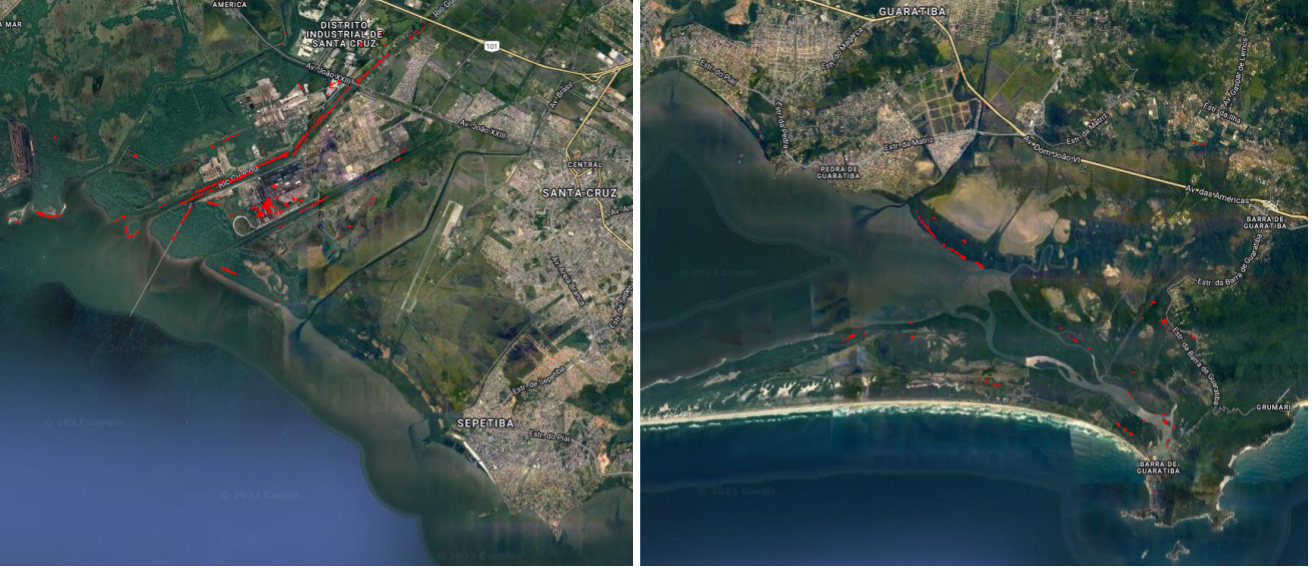
\includegraphics[width=0.95\textwidth]{Figures/chap4/loss_map.png}
\caption[Map of Mangrove Loss]{Map of Mangrove Loss from 2000 to 2018 as measured by Mean Anomaly \ac{ndvi}. Left: Ilha da Madeira, Santa Cruz, and Sepetiba. Right: Guaratiba and Pedra de Guaratiba.}
\label{fig:loss_map}
\end{figure}

\begin{figure}[!htb] 
\centering
\includegraphics[width=0.75\textwidth]{Figures/chap4/mangrove_photo.jpg}
\caption[Photo of Localized Mangrove Damage]{Photo of Localized Mangrove Damage. Taken by author during the August 2019 field visit.}
\label{fig:mangrove_photo}
\end{figure}


\paragraph{\hlc[cyan]{Mangrove Height}} \leavevmode\newline

The Simard et al. datasets were used to derive some general statistical information for the study area, including a distribution of heights, shown in \ref{fig:height_histogram}. Note that the $H_{max}$ values in particular contain a small number of outlier aberrations (no 40+ meter mangrove trees were visible during either of my field visits). Based on this data, the mean basal area weighted height of the mangroves in the study area is 7.4m while the mean maximum height is 11.6m. This compares to a mean height of 11.9m for the country of Brazil as a whole, according to Simard et al. \cite{simardMangroveCanopyHeight2019} suggesting that these trees are significantly shorter than those found in the northeastern Amazonian portion of the country.

\begin{figure}[!htb] 
\centering
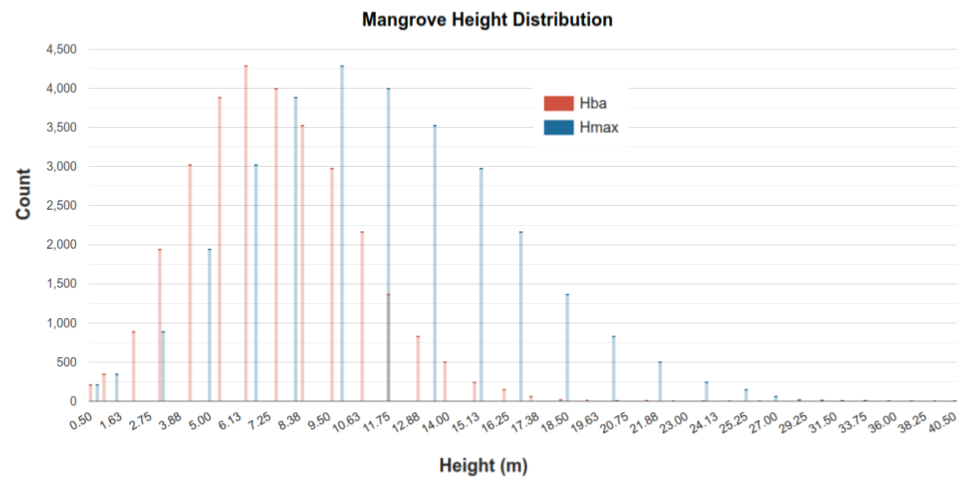
\includegraphics[width=0.95\textwidth]{Figures/chap4/height_histogram.png}
\caption[Histogram of Mangrove Height in Region]{Histogram of both the basal area weighted height ($H_{ba}$) and the maximum canopy height of each 30mx30m area ($H_{max}$).}
\label{fig:height_histogram}
\end{figure}

\paragraph{\hlc[cyan]{Mangrove Carbon Stocks and Sequestration}} \leavevmode\newline

As discussed in Section \ref{sec:rio-mangrove-carbon}, the above height data was used to estimate \ac{agb} and total carbon stocks for the region in 2018. The distribution of the total carbon stock density can be seen in Figure \ref{fig:carbon_density}, which roughly corresponds with the Figure \ref{fig:reference_median} map of median \ac{ndvi} during the reference period, as is to be expected. 

The calculation process resulted in an estimated total \ac{agb} for the region of 121000 MgC for the year 2000, compared to the Simard estimate of 95,000 MgC\footnote{Simard et al. do not specify whether they used the same allometric model to perform their \ac{rbag} calculations, as they propose several models. That said, I redid their calculations for the Guaratiba area and it does indeed seem that they used this same model.} \ac{agb} increased from to approximately 131,000 MgC (an 8.5\% increase). Total carbon meanwhile increased from 1,045,000 to 1,138,000 MgC (an 8.9\% increase). It should be noted that the \ac{agb} estimate is significantly lower than the estimate of 193,168 for the \ac{rbag} alone in Estrada et al. \cite{estradaEconomicEvaluationCarbon2015}. This estimate, which was based on an extent estimate for the year 2002 that are only slightly higher than that presented here, seems to differ primarily due to different allometric models. It is not implausible that these models, which were developed based on samples from within the \ac{rbag} are more accurate for this study area than the Americas generic power allometric model from Simard et al. \cite{simardMangroveCanopyHeight2019}. Unfortunately, Estrada et al.'s models are based on diamater at breast height, not height, and were only published for individual trees, not based on areal extent, making it difficult to replicate their calculation method or extend it to study changes over time. 

\begin{figure}[!htb] 
\centering
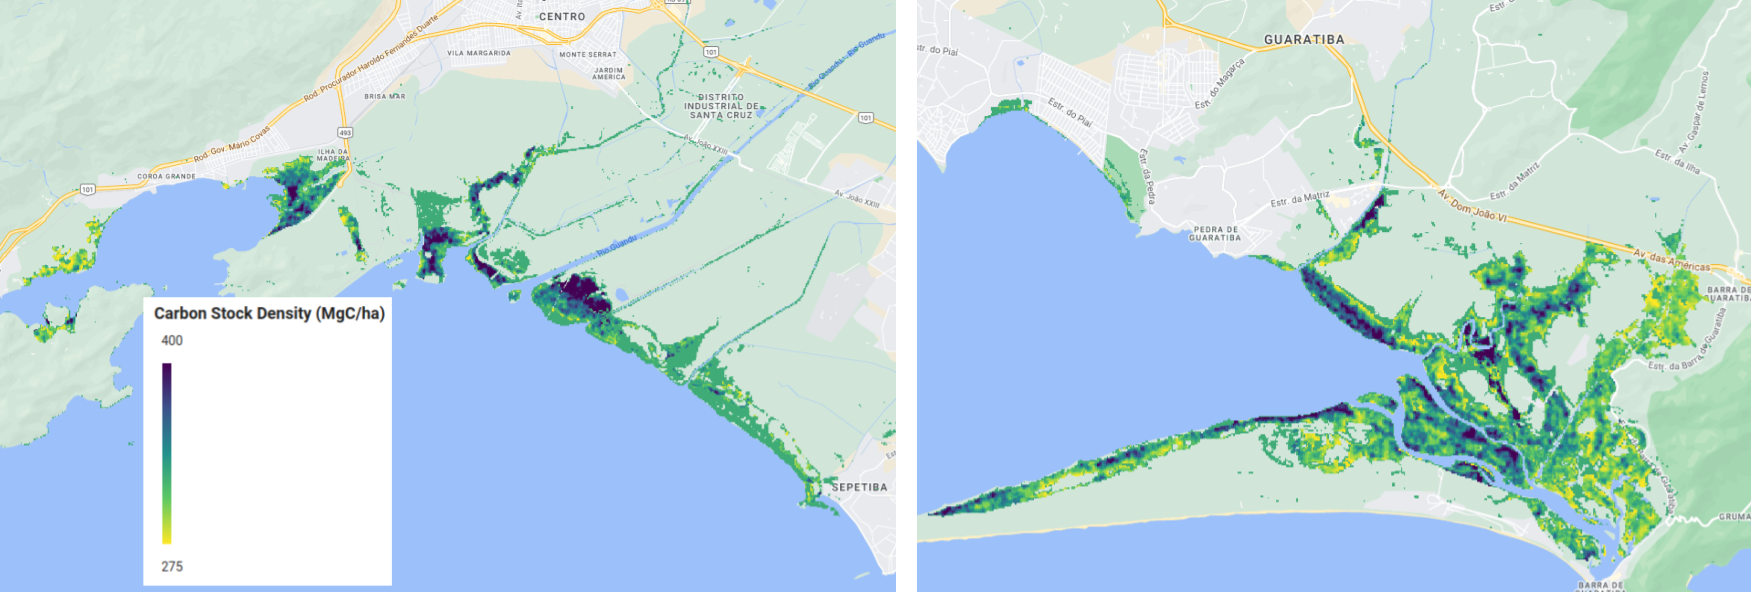
\includegraphics[width=0.95\textwidth]{Figures/chap4/carbon_density.png}
\caption[Mangrove Carbon Stock Distribution]{Mangrove carbon stock distribution for the 2018 extent. Left: Ilha da Madeira, Santa Cruz, and Sepetiba. Right: Guaratiba and Pedra de Guaratiba.}
\label{fig:carbon_density}
\end{figure}

Total carbon sequestration for the year 2018 is estimated at 20400 MgC. The lost 108 ha of mangroves represent 631 MgC/year or 3\% of the total. 

\subsubsection{\hlc[cyan]{Vulnerability}} 

\paragraph{\hlc[cyan]{Socioeconomic Situation}} \leavevmode\newline

In 2016 Guaratiba ranked 28 out of 32 of the \acp{ra} on the \ac{ips} with a score of 45.27 compared to the city-wide score of 60.77. This score is based on 36 indicators which are divided into three dimensions: Basic Human Necessities, Fundamentals of Well Being, and Opportunities. Figures \ref{fig:social_progress_indicator} and \ref{fig:ips_maps} shows how Guaratiba scores on each of these three dimensions relative to the other \acp{ra} of the city. The data that these scores are based on is available in \cite{institutopereirapassosBaseDadosIndice2022} and the methodology in \cite{puliciRelatorioMetodologicoIndice2016}.

\begin{figure}[!htb] 
\centering
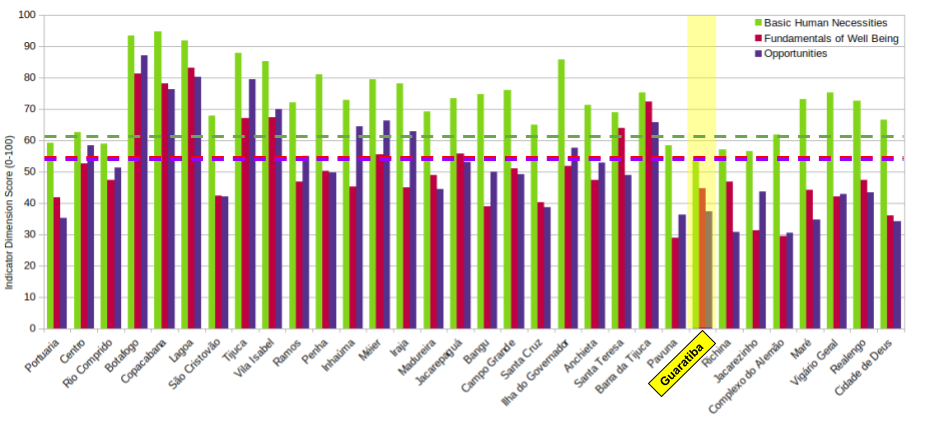
\includegraphics[width=0.95\textwidth]{Figures/chap4/social_progress_indicator.png}
\caption[Graph of Social Progress Indicator for Rio de Janeiro]{The \acf{ips} dimension scores for each \ac{ra} in Rio de Janeiro, with Guaratiba highlighted. Dashed lines indicate the city-wide score for the respective dimension.}
\label{fig:social_progress_indicator}
\end{figure}

\begin{figure}[!htb] 
\centering
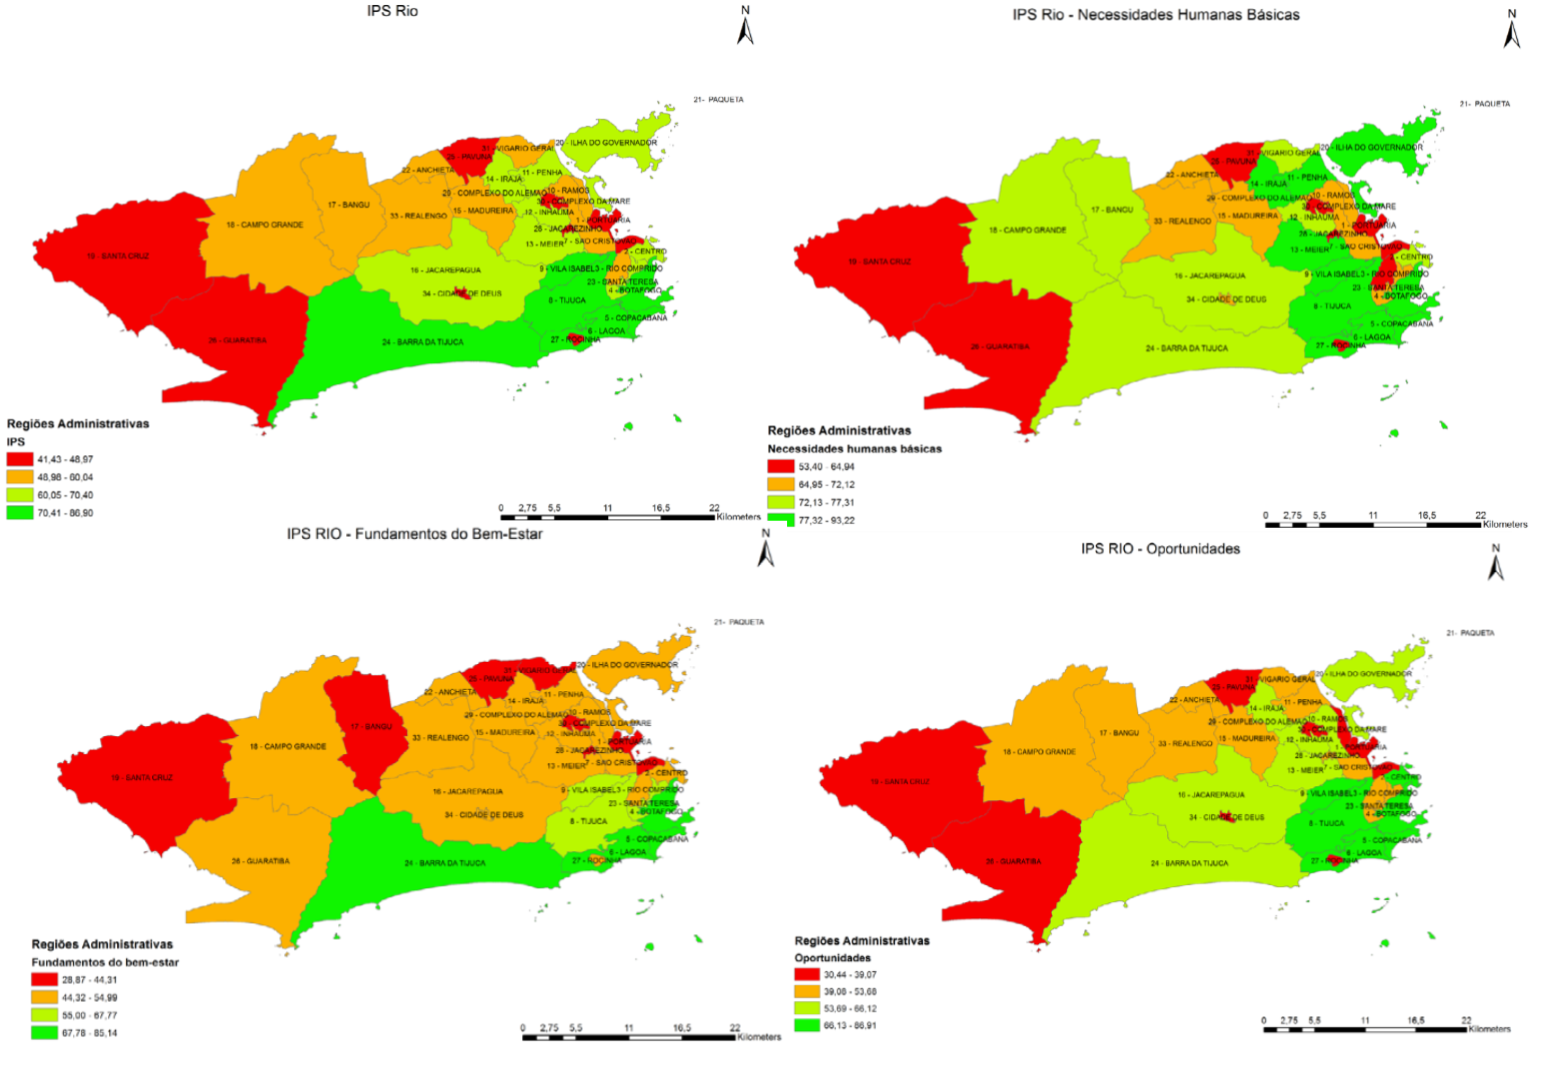
\includegraphics[width=0.95\textwidth]{Figures/chap4/ips_maps.png}
\caption[Map of Social Progress Indicator for Rio de Janeiro]{The \acf{ips} and dimension scores for each \ac{ra} in Rio de Janeiro. Guaratiba is visible in the bottom left of each map.}
\label{fig:ips_maps}
\end{figure}

Figure \ref{fig:agriculture_employment} meanwhile shows the rates of agricultural employment (relative to all forms of employment) in each bairro of the city. The bairros of Guaratiba and Barra de Guaratiba have rates of 5\% and 4\% respectively, well higher than the city-wide average of 0.01\% (acknowldging that these statistics do not capture all informal or subsistence activity). Overall this and the \ac{ips} scores indicate that Guaratiba is a socioeconomically vulnerable area with a likely heavy dependence on the natural environment. The following subsections will seek to determine the scale of this dependence on ecosystem services.

\begin{figure}[!htb] 
\centering
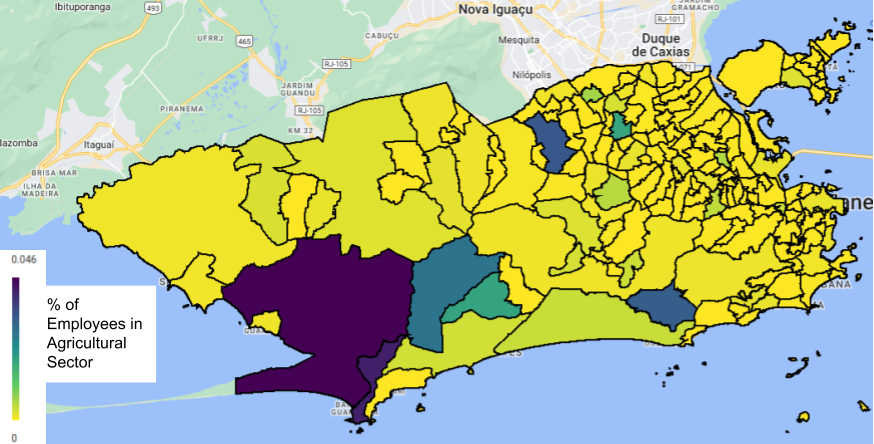
\includegraphics[width=0.95\textwidth]{Figures/chap4/agriculture_employment.png}
\caption[Agricultural Employment Across Rio de Janeiro]{Rates of Agricultural employment (relative to all employment) in each bairro in Rio de Janeiro for the year 2016.}
\label{fig:agriculture_employment}
\end{figure}

\paragraph{\hlc[cyan]{Carbon Regulation Ecosystem Services}} \leavevmode\newline

The estimated annual value of carbon sequestration for the study area over time can be seen in Figure \ref{fig:carbon_sequestration_value}. On average the mangroves sequester \$367K worth of carbon (in 2018 dollars) per year, for a total of \$6.97M USD (in 2018 dollars) for 2000 to 2018 period. This does not include the value of the stocks of carbon represented by the trees and soil itself, which are an estimated \$22.15M as of 2018, a \$1.82M increase compared to 2000.
    
\begin{figure}[!htb] 
\centering
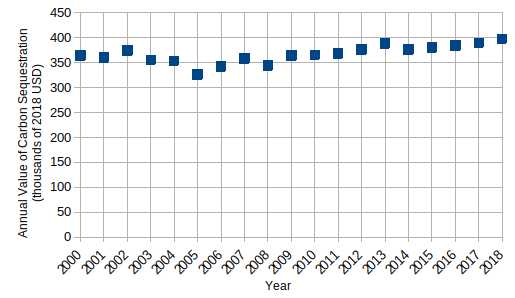
\includegraphics[width=0.95\textwidth]{Figures/chap4/carbon_sequestration_value.png}
\caption[Annual Value of Mangrove Carbon Sequestration]{Estimated annual value of mangrove carbon sequestration in the study area over time in thousands of 2018 USD.}
\label{fig:carbon_sequestration_value}
\end{figure}

\paragraph{\hlc[cyan]{Non-Carbon Ecosystem Services}} \leavevmode\newline


Using the ecosystem services rates from Souza \& Ramos e Silva \cite{souzaEcologicalEconomicValuation2011} for tourism, aquaculture, and tourism, meawhile, we find 2018 values of \$15.7K/year, \$33.9k/year, and \$60.3K/year, respectively, for a total of \$110M/year in non-carbon ecosystem services. How these values have changed over time, as well as a comparison to the value of the carbon stock that the mangroves represent in 2018 can be seen in Figure \ref{fig:annual_ecosystem_services}. Note that these do not include some other ecosystem services that are known to be present in the Guaratiba area, such as timber harvesting.

\begin{figure}[!htb] 
\centering
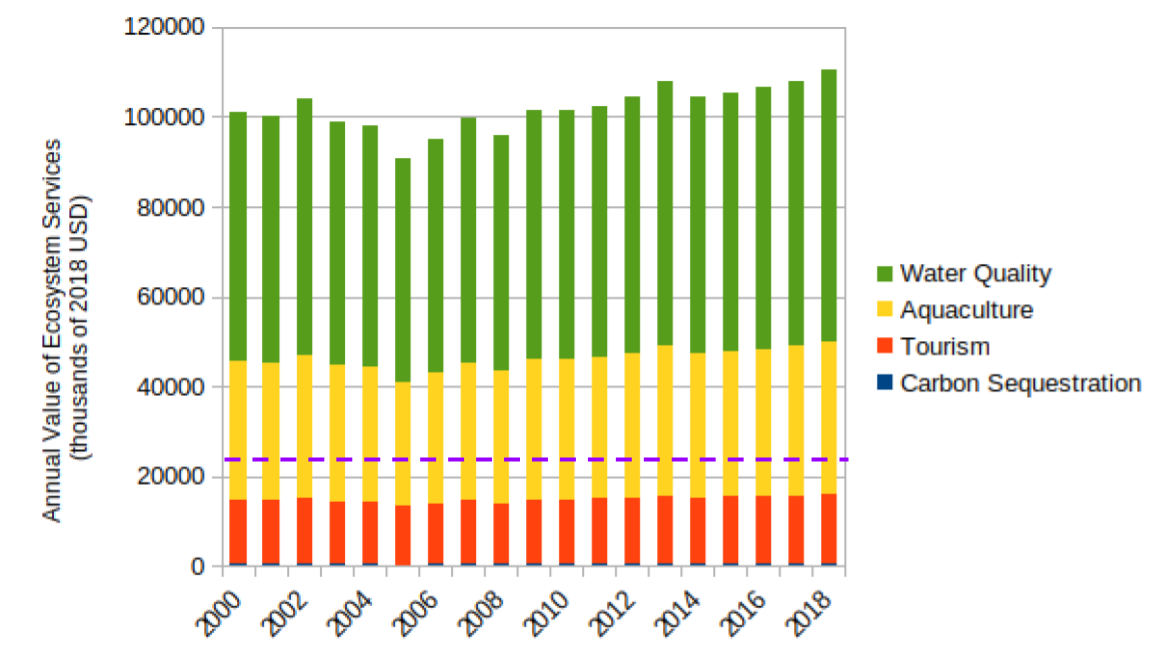
\includegraphics[width=0.7\textwidth]{Figures/chap4/annual_ecosystem_services.png}
\caption[Annual Value of Mangrove Ecosystem Services]{Estimated annual value of various mangrove ecosystem services in the study area over time in thousands of 2018 USD. The dashed line represents the estimated value of the mangrove carbon stocks in 2018.}
\label{fig:annual_ecosystem_services}
\end{figure}


\subsubsection{\hlc[cyan]{Decision-making}} \label{sec:rio-evdt-decision-results}

In order to discuss potential decisions regarding protected areas and zoning, or understand the impacts of such decisions, we must first understand their layout across the study area. \ac{smu} urban planning zones \cite{institutopereirapassosAreasProtegidas2021} and \ac{smac} environmentally protected areas \cite{institutopereirapassosSetores2022} are shown in Figure \ref{fig:zones}. These zone categories are based on the categories used by \ac{smu} with two primary differences. First, they are somewhat simplified. Each of these zone categories have various subcategories (e.g. Agriculture 1, Agriculture 2, etc.). I have reduced them to just \textit{Agriculture}. Similarly, \textit{Special and Misc.} is a synthetic category including special zones, areas of civil infrastructure construction, recycling centers, and much more. 

This leads to the second alternation that I made. Several of the coastal and near coastal zones are so-called ``Special Zones" that would by default be in the \textit{Special and Misc.} category. As this does would not be particularly useful for the purposes of this project, I reclassified some of them. Specifically the bulk of the mangroves of the \ac{rbag} are in ZE4 (Zona Especial 4). This is defined in law as essentially a tourism zone with certain alternations, namely that only single family residences are allowed, all buildings (except for hotels) will have a maximum of two floors, and development requires the approval of \ac{smu} \cite{prefeitodacidadedoriodejaneiroDecretoNo3221976}. For this reason, I reclassified it into the \textit{Tourism} category. ZE1 meanwhile includes all areas above a certain altitude (100m in this portion of the municipality). These are considered to be forest reserves and subject to federal jurisdiction \cite{prefeitodacidadedoriodejaneiroDecretoNo3221976}. I have thus reclassified them as \textit{Environmental Conservation}. ZE7 meanwhile refers to areas under the control of the Brazilian military. I have left this in \textit{Special and Misc.} but will note that this control results in some de facto levels of environmental protection, as discussed in Section \ref{sec:rio-jurisdictions}.

The environmental protection area categories meanwhile are unchanged from \ac{smac}'s systems. These categories are defined as:

\begin{itemize}[itemsep=0pt,parsep=0pt]
	\item{Proteção Integral: Literally ``comprehensive protection." Refers to environmentally significant areas in these areas little to no development or extractive activities are allowed.}
	\item{Tombamento: Literally ``asset area." Refers to areas that have important architectural, historical, or cultural importance. In this areas rules are in place to preserve whatever items or aspects warranted the classification.}
	\item{Zona de Amortecimento: Literally ``buffer zone." Refers to areas surrounding Proteção Integral areas in which certain (but not all) development and extractive activities are restricted to prevent impacting the adjacent environment.}
	\item{Uso Sustentável: Literally ``sustainable use." Refers to areas in which some development and extractive areas are restricted to reduce impact on the environment.}
\end{itemize}

\begin{figure}[!htb] 
\centering
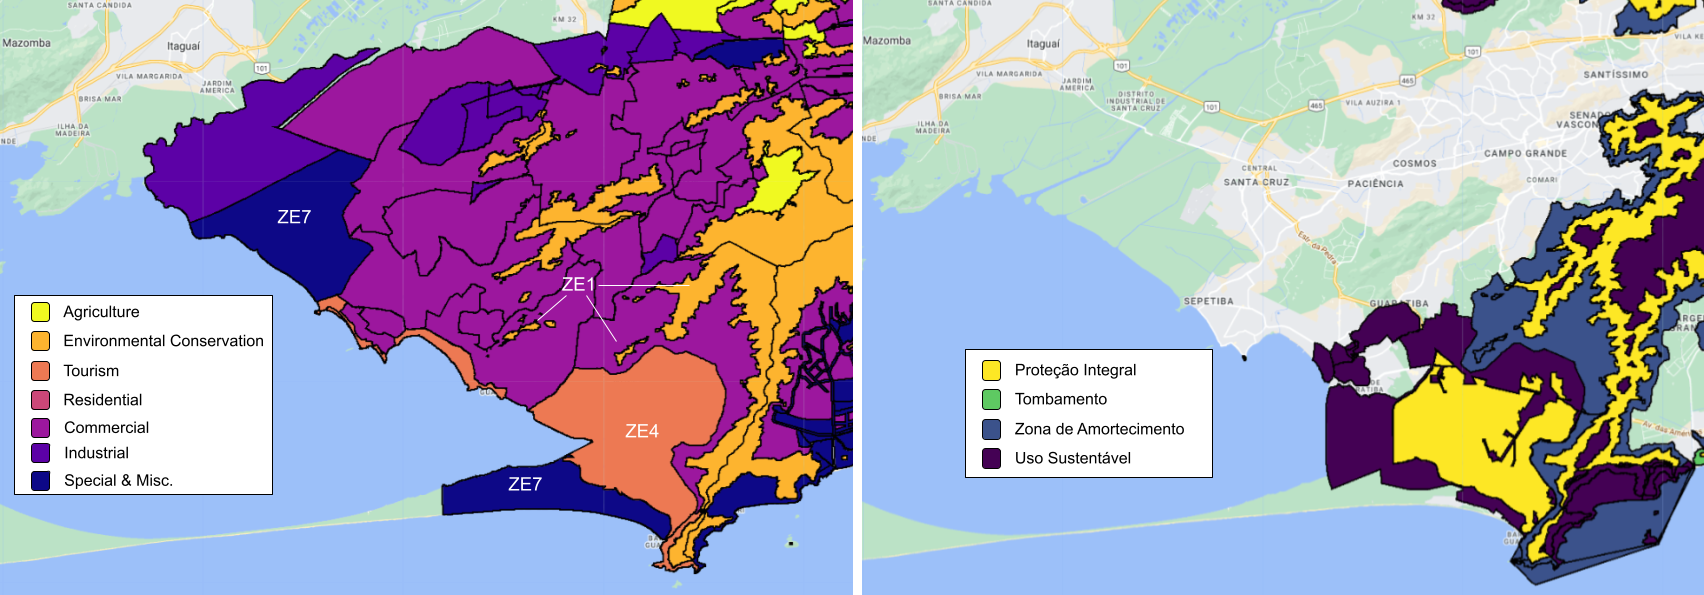
\includegraphics[width=0.95\textwidth]{Figures/chap4/planning_zones_and_protected_areas.png}
\caption[Planning Zones \& Protected Areas]{Left: Simplified map of the planning zones (governed by \ac{smu}). Right: Map of the environmentally protected areas (governed by \ac{smac}.}
\label{fig:zones}
\end{figure}

Tables \ref{tab:loss_area} and \ref{tab:loss_area_zone} show the extent, loss area, and relative loss of mangroves in each of the protected area and zone categories, respectively. For the protected areas, there does indeed seem to be a link between level of protection and prevention of loss, with the Proteção Integral and Tombamento areas experiencing the least losses (though there are so few mangroves in the Tombamento to begin with that they should be disregarded) and the Uso Sustentável and Zona de Amortecimento experiencing much higher loses. The gap between the these last two is the highest, suggesting a significant drop off in either policy restrictiveness or enforcement.

The zone categories should a similar trend, with \textit{Tourism} areas having the lowest losses and \textit{Industrial} areas having the highest. The relatively low losses of the \textit{Special \& Misc} category provide further evidence that military control of certain mangrove areas has a conservation effect, though not as much as explicitly protecting the mangroves.



\begin{table}[!htb]\centering
	\caption[Mangrove Extent and Loss by Protected Area Category]{Mangrove Extent and Loss by Protected Area Category.} \label{tab:loss_area}
	% \small
	\fontsize{8}{10}\selectfont
	\csvreader[tabular=|C{3cm}|C{2cm}|C{2cm}|C{2cm}|, 
		table head=\hline 
		\textbf{Protected Area Category} & \textbf{Mangrove Extent (ha)} & \textbf{Mangrove Loss (ha)} & \textbf{Relative Loss (\%)} \\ \hlinewd{2pt},
		table foot=\hline,
		late after line=\\\hline]
		{Figures/chap4/area_and_loss_by_protected_sums.csv}
		{1=\year,2=\type,3=\platform,4=\agency}
		{\textbf{\year} & \type & \platform & \agency}
\end{table}

\begin{table}[!htb]\centering
	\caption[Mangrove Extent and Loss by Zone Category]{Mangrove Extent and Loss by Zone Category.} \label{tab:loss_area_zone}
	% \small
	\fontsize{8}{10}\selectfont
	\csvreader[tabular=|C{3cm}|C{2cm}|C{2cm}|C{2cm}|, 
		table head=\hline 
		\textbf{Zone Category} & \textbf{Mangrove Extent (ha)} & \textbf{Mangrove Loss (ha)} & \textbf{Relative Loss (\%)} \\ \hlinewd{2pt},
		table foot=\hline,
		late after line=\\\hline]
		{Figures/chap4/area_and_loss_by_zone_sums.csv}
		{1=\year,2=\type,3=\platform,4=\agency}
		{\textbf{\year} & \type & \platform & \agency}
\end{table}



%[** consider adding in this figure and discussion somewhere]
%Figure \ref{fig:informal_settlements} shows the boundaries of informal settlements through the study area for the year 2017 \cite{LimiteFavelas20172019}.
%
%\begin{figure}[!htb] 
%\centering
%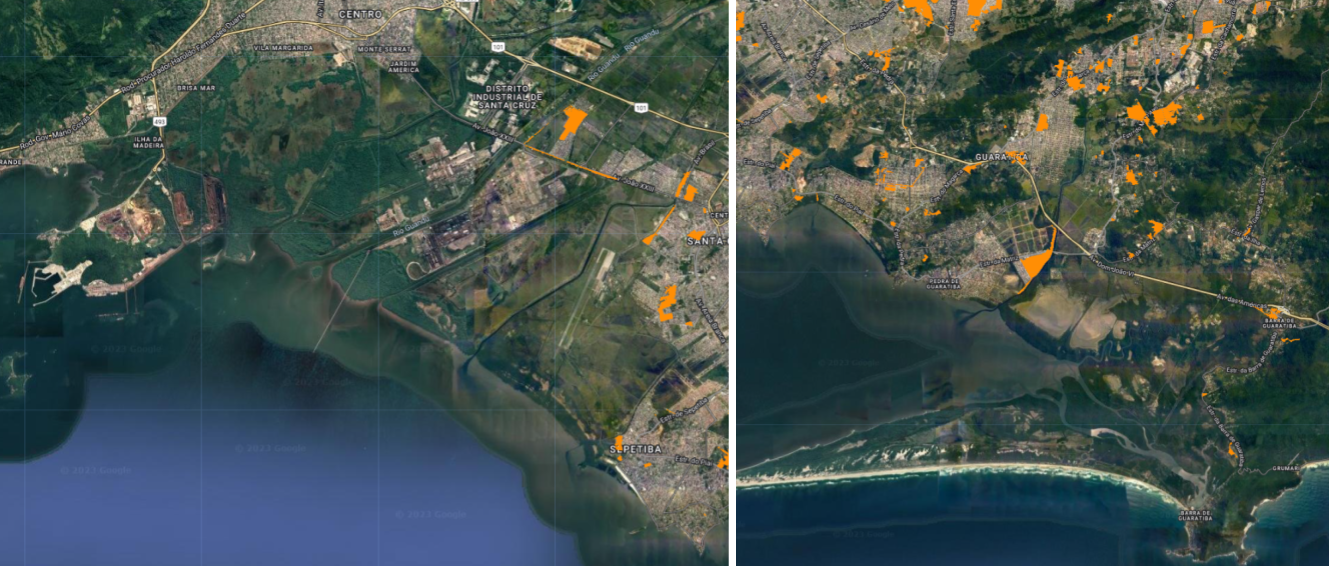
\includegraphics[width=0.7\textwidth]{Figures/chap4/informal_settlements.png}
%\caption[Informal Settlements]{Informal settlements throughout the study area in 2017. Left: Ilha da Madeira, Santa Cruz, and Sepetiba. Right: Guaratiba and Pedra de Guaratiba}
%\label{fig:informal_settlements}
%\end{figure}


\subsubsection{\hlc[cyan]{Technology}} 

The city government of Rio de Janeiro has made significant use of \ac{eo} data dating back to 1975, as can be seen in Table \ref{tab:history}, but it is only in recent years that this data usage has become fairly regular. This regularization roughly corresponds with the creation of \ac{ipp} in 1999. Even now, there has not been any particular consistency with the choice of imagery source, with the city switching back and forth between aerial and satellite surveys every few years. The primary use of this data, \acf{lclu} classification, was performed via a combination of updating previous \ac{lclu} maps, visual classification of the imagery, and in-situ surveys.

There have also been some efforts outside of remote observation. \ac{smac} has recently been experimenting with a process for integrating photos taken by cell phones into forest degradation monitoring. The ESPAÇO research group has been conducted \ac{uav} surveys of certain portions of mangrove forest, with particular interest in photogrammetry. 

Certain aspects of this use history are worth noting. First, there has been little to no active monitoring of the city or environment at anything approximating a real-time pace. Based on the stakeholder analysis conducted in Section \ref{sec:rio-saf}, this is likely due to a combination of lack of perceived need, cost, and lack of capacity (the last primarily being the result the former two). The pace at which a city government operates and at which many of the relevant environmental phenomena develop simply do not typically necessitate daily, weekly, or even monthly imagery.

Second, outside of the occasional use of Landsat series imagery by \ac{smac} for forest health monitoring via \ac{ndvi} (particularly deforestation and fire measurements), there has been a noticeable lack in the use of civil scientific satellites such as Landsat for mapping and decision-making purposes. This is partially a matter of spatial resolution. As can be seen in Table \ref{tab:history}, most of the imagery used has an order of magnitude finer resolution than the 30m of the Landsat series. This limitation of civil satellites for urban use is by no means unique to Rio de Janeiro or new, as was discussed in Section \ref{sec:remote}. That said, there are a variety of potentially useful analysis methods beyond manual visual classification or a basic \ac{ndvi} interpretation (including those used shown earlier in this chapter in Section \ref{sec:rio-evdt-e-method}). The lack of such methods may indicate either difficulty in accessing the civil imagery or a lack of capacity for working with them.

\begin{table}[!htb]\centering
	\caption[EO data use by Rio de Janeiro]{\ac{eo} data use by municipal government agencies of Rio de Janeiro}\label{tab:history}
	% \small
	\fontsize{8}{10}\selectfont
	\csvreader[tabular=|C{1.75cm}|L{3cm}|L{4cm}|C{1.75cm}|L{3cm}|, 
		table head=\hline 
		\textbf{Year(s)} & \textbf{Product} & \textbf{Platform} & \textbf{Collecting Agency} & \textbf{Primary Use} \\ \hline,
		table foot=\hline,
		late after line=\\\hline]
		{Figures/chap4/eo_history.csv}
		{1=\year,2=\type,3=\platform,4=\agency,5=\primary}
		{\year & \type & \platform & \agency & \primary}
\end{table}


\section{\hlc[cyan]{Decision Support System}} \label{sec:rio-dss}

The lessons, data, and analysis from the \ac{saf} (Section \ref{sec:rio-saf}) and the \ac{evdt} framing (Section \ref{sec:rio-evdt}) were used to design and develop a \acf{dss}. To revisit the System Functions, the primary functions of the \ac{dss} were to:

\begin{itemize}[itemsep=0pt,parsep=0pt]
    \item{\textbf{Descriptively model environmental phenomena}, in particular mangrove health trends over the past two decades. This will inform the current state of the environment and possible future trajectories.}
    \item{\textbf{Provide estimates of mangrove ecosystem services}, including both local and global services. This will help inform decision-making around mangroves by various stakeholders.}
    \item{\textbf{Generate potential future conservation scenarios.}}
\end{itemize}

Much of the development took place in fall of 2019 and spring of 2020, including some rapid iterations involving stakeholders during my March 2020 field visit. Both this field visit and the development of the \ac{dss} were cut short by the onset of the coronavirus pandemic. The \ac{dss} should thus be viewed as an incomplete product with significant room for improvement, as will be discussed further in Section \ref{sec:rio-discussion}.

\subsection{\hlc[cyan]{Overview of Components and Initialization}}

The \ac{dss} was created as an open-source desktop/laptop-based application written in the Python programming language and making heavy use of the tkinter package. This package allows for the creation of a Tk \ac{gui}, which enables a common user experience on Linux, Windows, and macOS. It can be run either by downloading and running the complete \ac{dss} Python package or through the use of an executable compiled with PyInstaller. All codes is available at [**insert code repository]. The display language is in Brazilian Portuguese as this is the most common language known to the stakeholders.

The \ac{dss} consists of three primary components:

\begin{enumerate}[label=\emph{\alph*},itemsep=0pt,parsep=0pt]
	\item{\textbf{A map display} capable of showing a variety of both raster and vector data including a a satellite view of the area, jurisdictional boundaries, chloropleth statistics, and mangrove extent and health. It is capable of zooming in and out on a user selected point. By default it includes most of the study area, stretching from Ilha da Madeira to Barra de Guaratiba.}
	\item{\textbf{A text display} of various demographic, economic, and environmental data at any location selected by the user.}
	\item{\textbf{A simulator} capable of generating future scenarios for the year 2028 and displaying them via the above two components. These scenarios were based the user selectively altering the categories of the protected areas and planning zones. Only a rudimentary such simulator was developed prior to the project cutoff.}
\end{enumerate}

All three such components are immediately presented to the user upon initialization, as seen in Figure \ref{fig:rio-dss-startup-screenshot}. The software steps that take place during this initialization are described in detail in Figure \ref{fig:ui_flowchart_initialization}. This layout and the underlying functions were developed in an iterative process with stakeholders, involving mockups, proofs-of-concepts, and quick revisions. Figure \ref{fig:mockup} shows two examples of such mockups, dating back to before the decision was made to display Portuguese instead of English. These were used to ensure user intelligibility and usability at each step of the development process. 

\begin{figure}[!htb] 
\centering
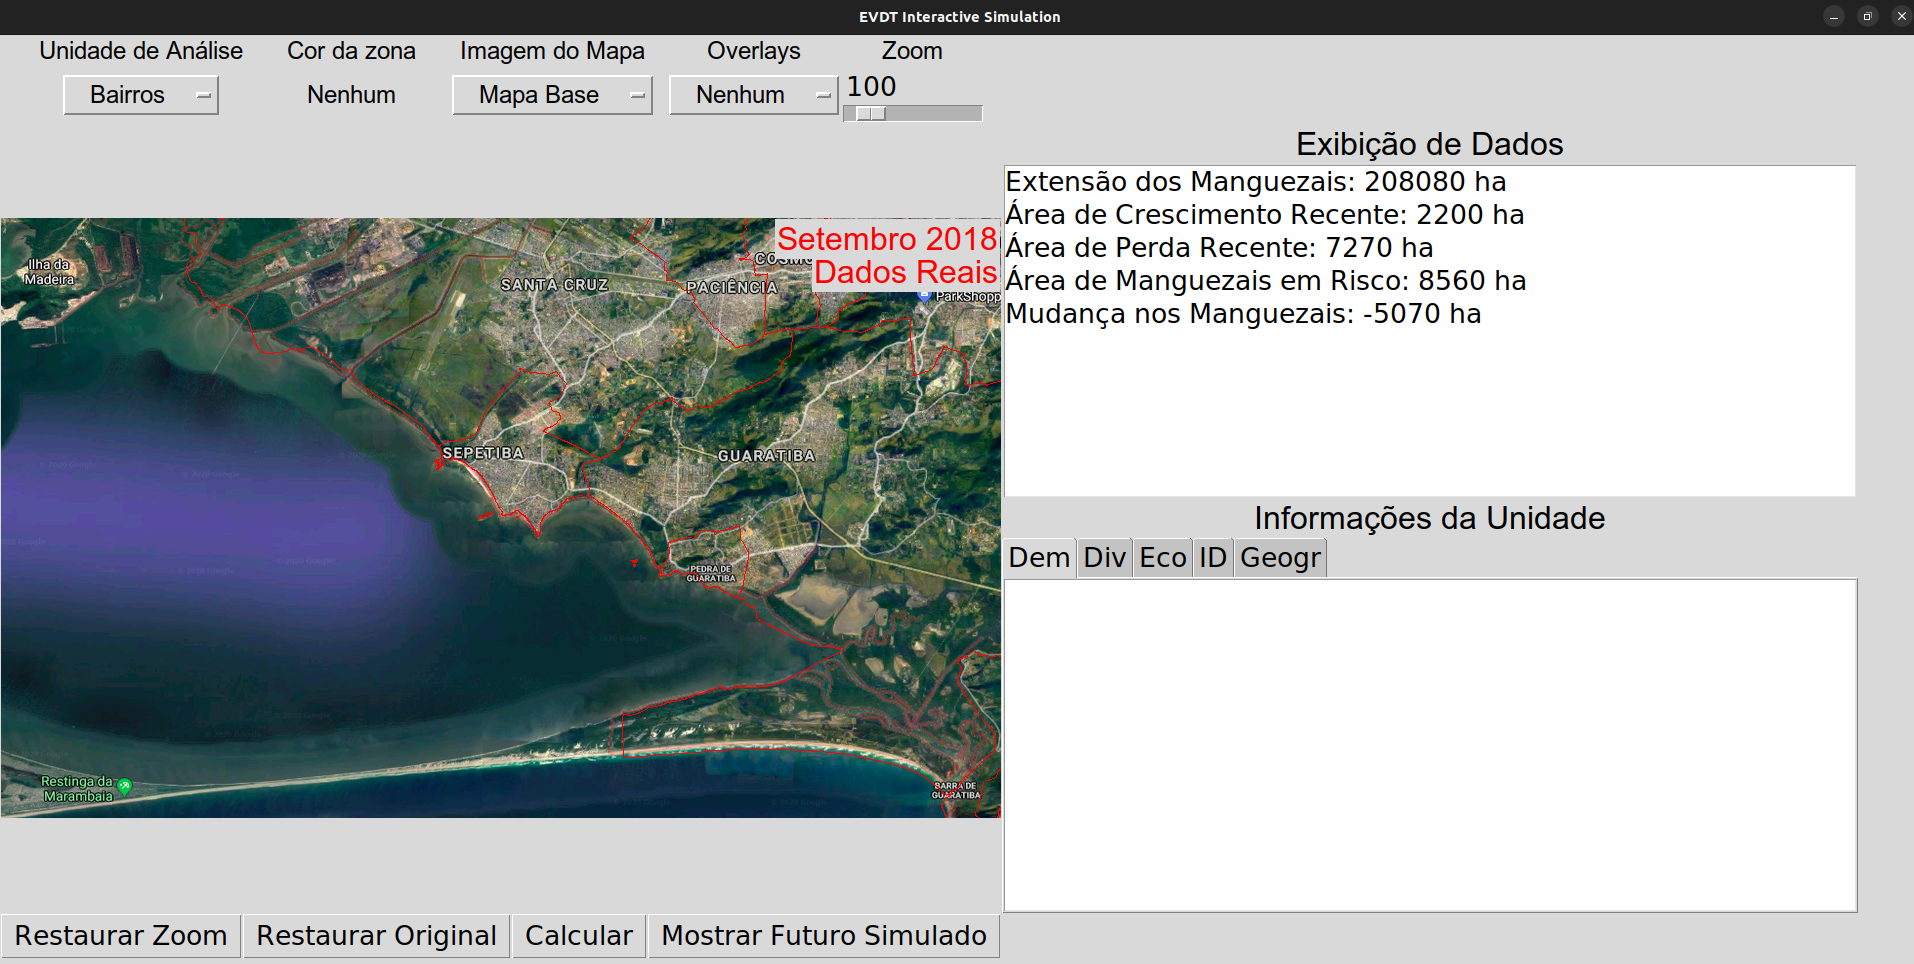
\includegraphics[width=0.95\textwidth]{Figures/chap4/rio-dss-startup-screenshot.png}
\caption[Screenshot of Startup Screen of the Rio de Janeiro DSS]{Screenshot of the \ac{dss} prototype's startup screen.}
\label{fig:rio-dss-startup-screenshot}
\end{figure}

\begin{figure}[!htb] 
\centering
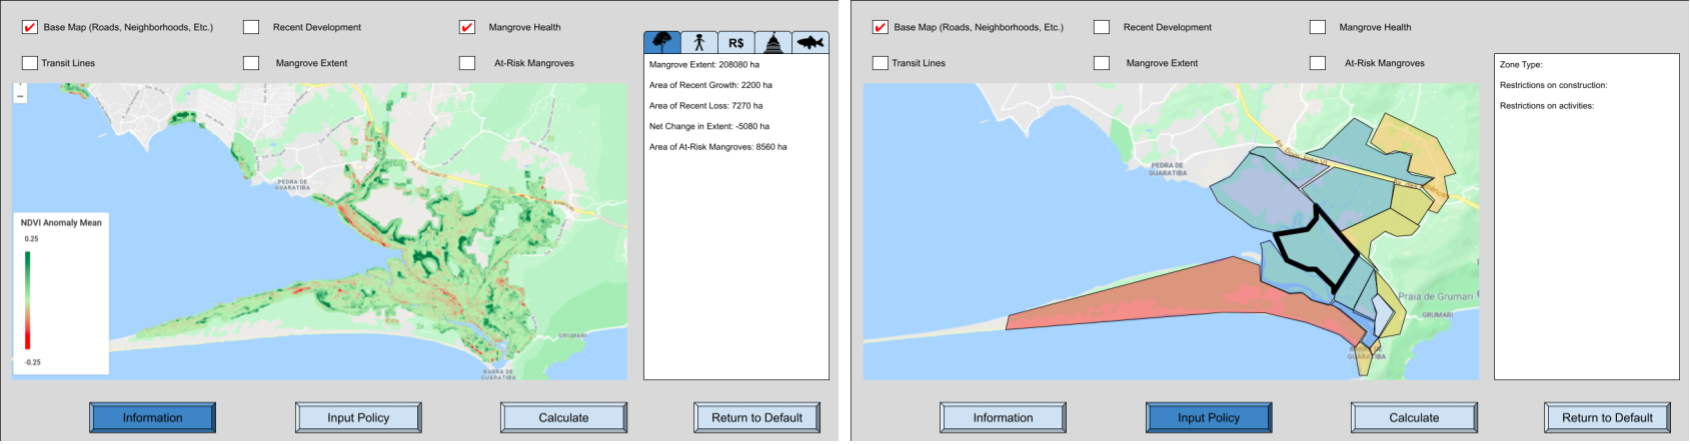
\includegraphics[width=0.95\textwidth]{Figures/chap4/display_and_input.png}
\caption[Rio DSS Mockups]{Mockups of the \ac{dss} used during the development process. Left: How both spatial and nonspatial information might be displayed. Right: How user inputs on protected areas and zoning might appear.}
\label{fig:mockup}
\end{figure}

\subsection{\hlc[cyan]{Spatial and Textual Data Display}}

In order to explain the various information display functions of the \ac{dss}, I will refer to the Figure \ref{fig:rio-dss-screenshot} screenshot, which represents the state of the \ac{dss} after the user has made various data selections. Drop-down menus in the top left allow the user to control:

\begin{itemize}[itemsep=0pt,parsep=0pt]
	\item{\textbf{Unidade de Análise:} The spatial unit of analysis. This dictates both what chloropleths are available and what information is available in the \textit{Informações da Unidade} box on the bottom right. Options are bairros (neighborhoods), Áreas Protegidas (the environmentally protected areas), and Zonas de Planejamento (the urban planning zones). In this screenshot, the Áreas Protegidas are selected, resulting in corresponding red outlines on the map.}
	\item{\textbf{Cor da zona:} The metric on which the chloropleth is based. What options are available depend on the Unidade de Análise selected. The full listing is shown in Table \ref{tab:rio-dss-data}. Here the classification of the protected areas, as defined in Section \ref{sec:rio-evdt-decision-results}, is selected, resulting in the various shades of green. It is also possible to select none, in which case the units of analysis will be transparent.}
	\item{\textbf{Imagem do Mapa:} The underlying image of the region. In this version the only two options where the Google Maps Satellite view (shown here) or none.}
	\item{\textbf{Overlays:} Data derived from spatial raster sources that can be overlain on the map. The options are mangrove health (as measured by \ac{ndvi} mean anomaly from 2000 to 2018), mangrove loss from 2000 to 2018, or none. Here mangrove health is selected.} 
\end{itemize}

\begin{figure}[!htb] 
\centering
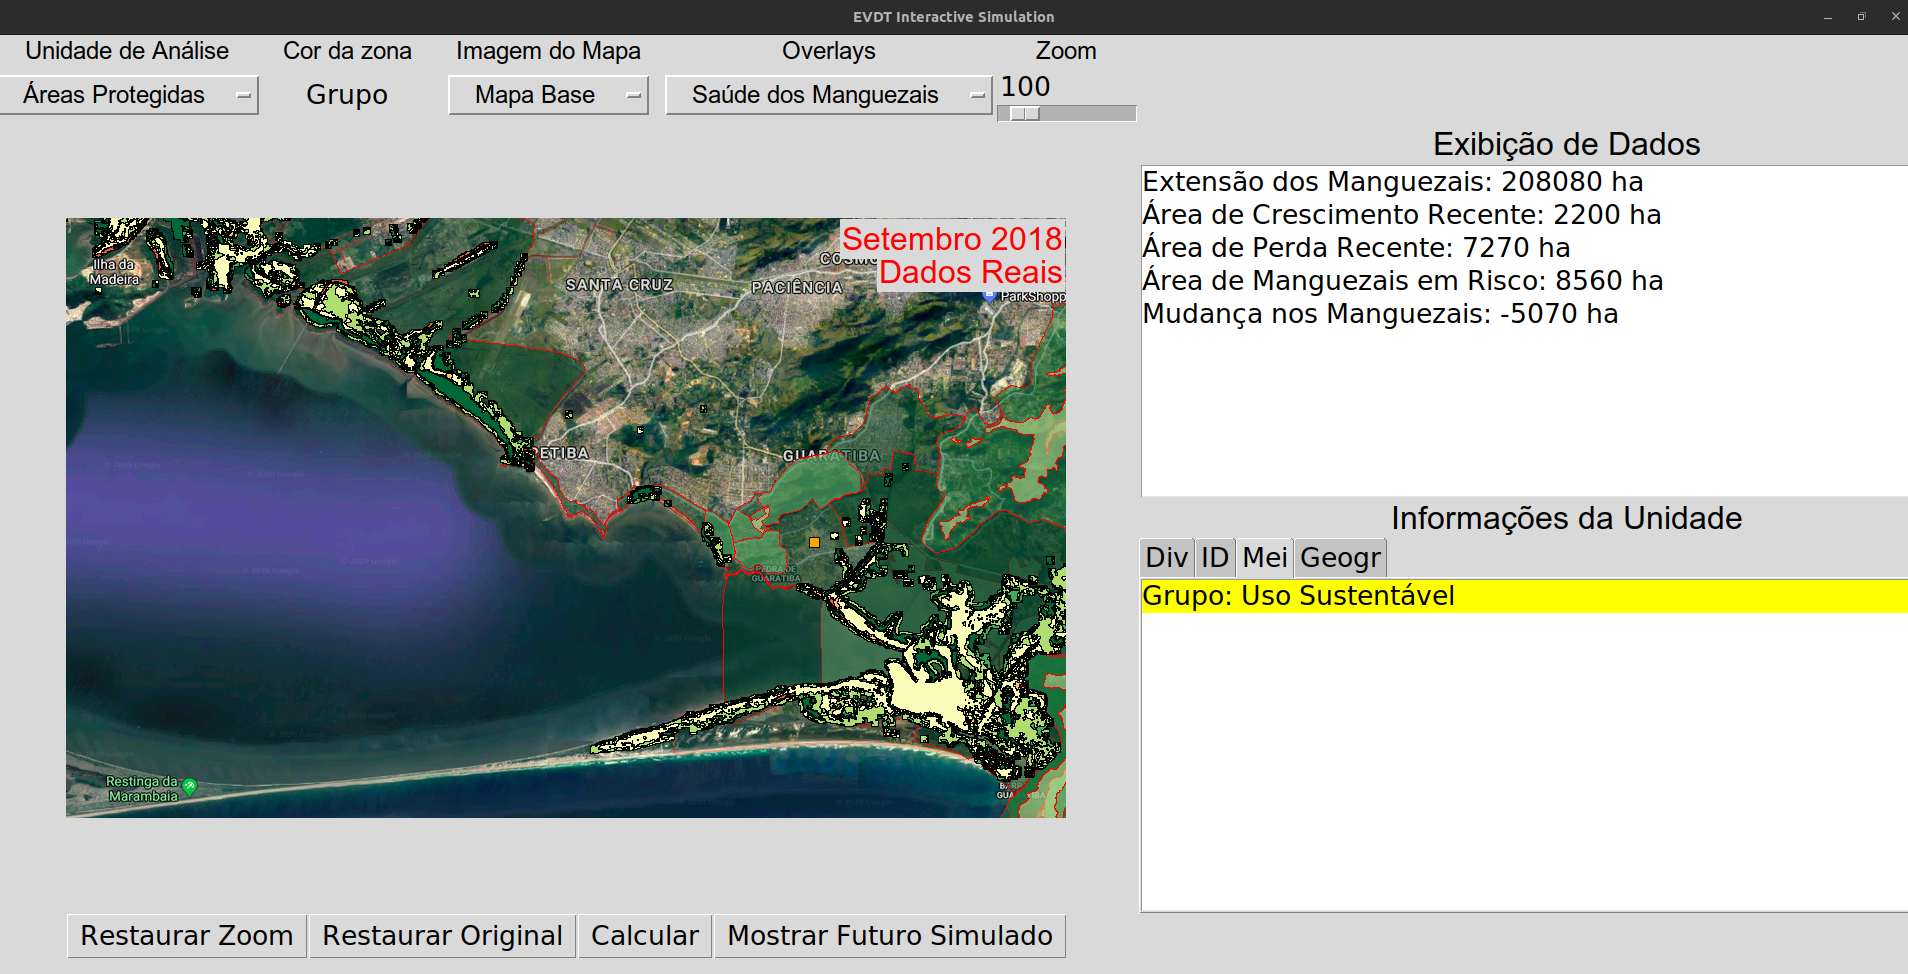
\includegraphics[width=0.95\textwidth]{Figures/chap4/rio-dss-screenshot.png}
\caption[Screenshot of Rio de Janeiro DSS]{Screenshot of the \ac{dss} prototype. The orange square indicates where the user has selected.}
\label{fig:rio-dss-screenshot}
\end{figure}

\begin{table}[!htb]
\caption[Data Displayed by the Rio DSS]{Data available for display by the \ac{dss}, sorted by the unit of analysis and the category of data. Bolded entries indicate what variables a user is able to edit for the purposes of scenario generation. This table is written in English and thus does not directly match the Portuguese labels seen in the screenshots of the actual \ac{dss}.}
\label{tab:rio-dss-data}
\begin{center}
\scriptsize
\begin{tabular}{| C{3cm} |  L{4cm} | L{4cm} |} \hline
 
\textbf{Unit of Analysis} & \textbf{Data Categories} & \textbf{Available Data}  \\ \hlinewd{2pt}

\multirow{11}{*}{Neighborhoods} & ID & Name \\ \hline
& \multirow{2}{*}{Demographics} & Population \\
& & Population Density \\ \hline
& \multirow{4}{*}{Economy} & 2017 Agriculture Workers \\
& & 2017 Number Employed \\
& & 2017 Proportion of Agriculture Jobs \\
& & 2017 Employment Rate \\ \hline
& \multirow{2}{*}{Geography} & Area of Unit \\ 
& & Mangrove Loss \\ \hline
& \multirow{2}{*}{Miscellaneous} & \acf{ra} \\
& & \acf{ap} \\ \hline

\multirow{7}{*}{Protected Areas} & ID & Name \\  \hline
& Environmental & \textbf{Group} \\  \hline
& \multirow{2}{*}{Geography} & Area of Unit \\ 
& & Mangrove Loss \\ \hline
& \multirow{3}{*}{Miscellaneous} & Jurisdiction (municipal, state, or federal) \\
& & Creation Method (municipal legislation, federal regulation, etc.) \\
& & Creation Number (statute, code, etc.) \\ \hline

\multirow{4}{*}{Planning Zones} & ID & Zone ID Number \\ \hline
& Economy & \textbf{Group} \\ \hline
& \multirow{2}{*}{Geography} & Area of Unit \\ 
& & Mangrove Loss \\ \hline
& Miscellaneous & Governing Legislation \\ \hline

\end{tabular}
\end{center}
\end{table}

The user can select any location on the map, resulting in an orange square indicator being placed there. Once this has been done, the user can zoom in or out using the slider in the top-center. The map zoom level and focus can be reset by clicking the \textit{Restaurar Zoom} button in the bottom left. Various data available for the selected unit of analysis will populate the different tabs of the \textit{Informações da Unidade} box on the bottom right. 

The \textit{Exibição de Dados} (Data Exhibit) in the top right shows a variety of information about the entire study area. In the Figure \ref{fig:rio-dss-screenshot}, this includes the 2018 mangrove extent, the area of recent growth, the area of recent loss, area of mangroves at risk of loss, and the net change in mangroves since 2000\footnote{This figures shown in this screenshot are from an older analysis and with a slightly different study area and period. They thus do not match the values reported in Section \ref{sec:rio-evdt-e-result}.}. 

\subsection{\hlc[cyan]{Scenario Generation}}

In order to generate a future scenario for the year 2028, the user simply clicks the \textit{Calcular} button in the bottom center of the interface. After a period of calculation, the \ac{dss} display will transition from showing real world data to simulated data, as seen in Figure \ref{fig:rio-dss-simulation}. Note that the redtext in the top right of the map specifies both the date of the displayed information and whether the information is real or simulated.

In this prototype, the scenario generation process consists of a highly simplistic toy model in which mangrove health increases, remains the same, or decreases depending on the combination of environmental protection area category and the planning area category that the mangrove is present in. The directionality and magnitude of these changes are roughly based on the correlations noted in Section \ref{sec:rio-evdt-decision-results}. 

\begin{figure}[!htb] 
\centering
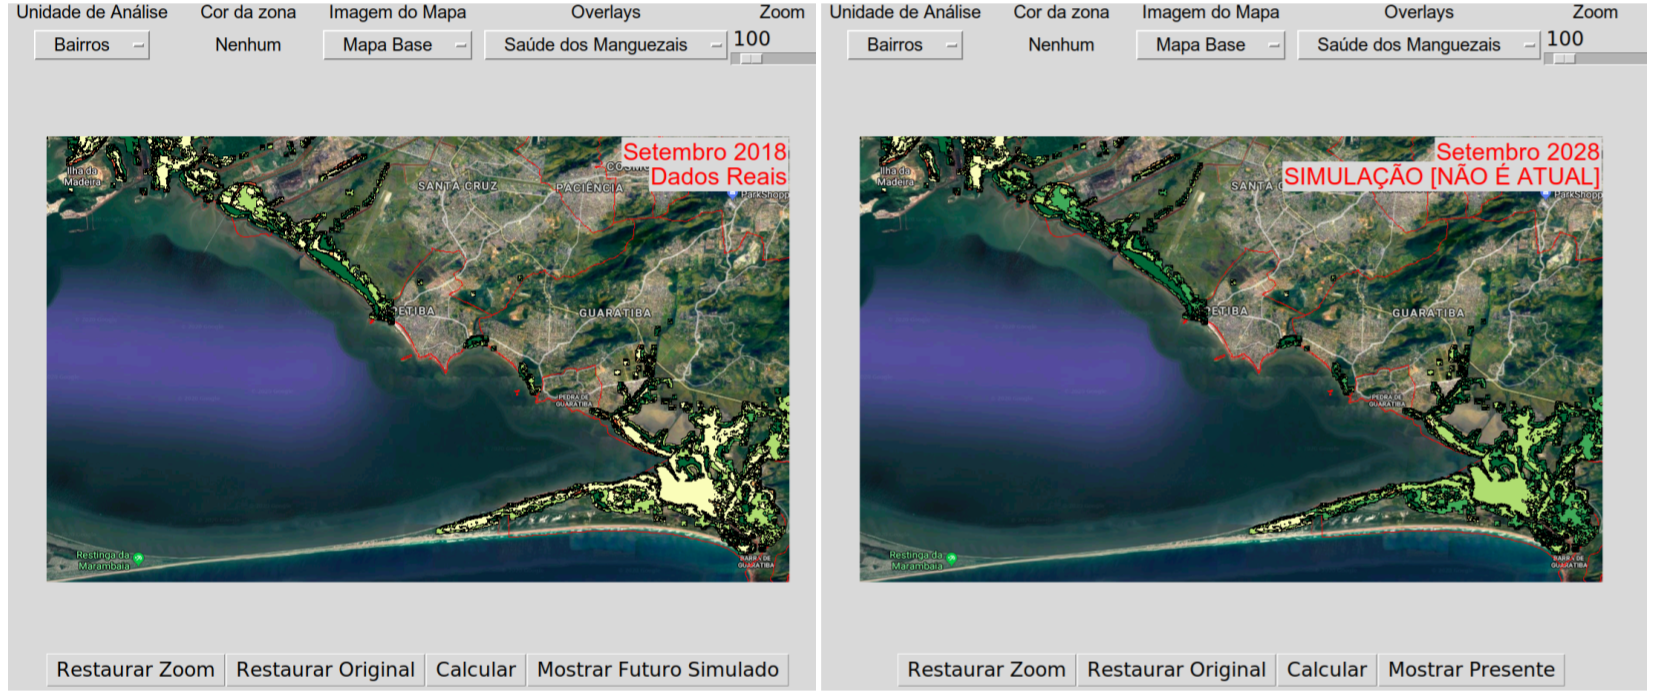
\includegraphics[width=0.95\textwidth]{Figures/chap4/rio-dss-simulation.png}
\caption[Demonstration of the Rio DSS Scenario Generation]{Left: A screenshot of the \ac{dss} prior to scenario generation. Right: A screenshot of the \ac{dss} after scenario generation.}
\label{fig:rio-dss-simulation}
\end{figure}

By default, the scenario generation process assumes that there are no policy changes (i.e. the types and boundaries of both the protected areas and planning zones do not change). The user can, however, alter the types of the protected areas and/or planning zones at their discretion. To accomplish this, the user must first switch the map to the appropriate unit of analysis type (using the \textit{Unidade de Análise} drop-down menu in the top-left), and then click on the particular desired unit on the map. Now, in the \textit{Informações da Unidade} box, the variables available for alteration will be highlighted in yellow, as seen in Figure \ref{fig:rio-dss-screenshot}. The user can click on such variables and change them to any of the other policy categories listed in Section \ref{sec:rio-evdt-decision-results}.

Once the user has altered the protected areas and planning zones to their desire, they can generate the new scenario by clicking on the \textit{Calcular} button. If they wish to go back and try different inputs, the \textit{Restaurar Original} resets the scenario back to 2018. If they wish to visually compare the real world 2018 data to the simulated 2028 scenario, the \textit{Mostrar Futuro Simulado / Mostrar Presente} button allows them to switch back and forth without having to repeat the scenario generation process.

The full set of user actions, along with the resulting software processes, are detailed in Figure \ref{fig:ui_flowchart_user_actions}.

\begin{landscape}

\begin{figure}[t] 
\centering

\includegraphics[scale=0.2]{Figures/chap4/ui_flowchart_initialization}
\caption[Flowchart of Rio DSS Initialization]{Flowchart showing the initialization process of the Rio \ac{dss}. Note: This figure is a vector image that should support significant zooming in the PDF version of this thesis.}
\label{fig:ui_flowchart_initialization}
\end{figure}

\begin{figure}[t] 
\centering
\includegraphics[scale=0.075]{Figures/chap4/ui_flowchart_user_actions}
\caption[Flowchart of Rio DSS Actions]{Flowchart showing the various actions that a user of the \ac{dss} can perform and how the system executes them. Note: This figure is a vector image that should support significant zooming in the PDF version of this thesis.}
\label{fig:ui_flowchart_user_actions}
\end{figure}
\end{landscape}

\section{\hlc[cyan]{Collaborative Development Process}} \label{sec:rio-collab}

As explained in Section \ref{sec:evdt-collab}, the \ac{evdt} Framework calls for stakeholder engagement, participation, and collaboration throughout the project. This starts with that initial contacts, meetings, discussions, and interviews that make up the Stakeholder Analysis step of the \ac{saf}. Such activities for this case study were detailed previously in Section \ref{sec:rio-saf}. Collaboration does not end there, however, and several other forms of stakeholder involvement were relied upon for this project.

With \ac{ipp}, regular one-on-one meetings were held with myself and Felipe Mandarino throughout this project and the Vida project detailed in Chapter \ref{ch:vida}. The frequency of these meetings fluctuated from weekly to monthly depending on the needs of this project and our other professional responsibilities. These meetings were used to demonstrate and critique prototypes of the \ac{dss}, discuss potential additional datasets, and plan ways of engaging other stakeholders.

During my field visits in 2019 and 2020, I also spent significant time in the offices / workspace of \ac{ipp}, ESPAÇO, and \ac{smac}. This enabled me to observe the day-to-day work life of these stakeholders, learn more about the work that they do (both relevant to this project and not), and get direct input and feedback on the \ac{dss} and \ac{evdt} analyses. 

During these visits, I also had the opportunity to visit the mangroves of Guaratiba and the surrounding communities multiple times. One of these trips involved an ESPAÇO-led tour of the \ac{rbag} and an \ac{uav} photogrammetry survey of a portion of the mangrove forest near the Araçatiba settlement. A later trip involved a tour led by a local fisher of Pedra de Guaratiba, the eastern portion of the Sepetiba bay, and some of the mangroves surrounding the bay. Over the course of both of these visits, stakeholders shared information about their socioeconomic status, their relationship with the mangroves, and their hopes for the future. I was also able to directly observe how the mangroves and their associated environment was being used.

Additional correspondence with \ac{smac}, \ac{smu}, ESPAÇO, and \ac{ipp} took place over email and video conference calls throughout the duration of the project. Finally, various stakeholders were invited to participate (and in fact did so) with the monthly \ac{evdt} community meetings once those began in 2022 (see Chapter \ref{ch:vida} for more discussion of these meetings). 

It is recognized that this level of collaboration fell short of what was originally envisioned at the onset of this project. Part of this was the onset of the coronavirus pandemic which cut short the project and resulted in my departure from the second visit early. This prevented a series of future rounds of interviews and workshops with stakeholders. The first of these would have revisited each of the stakeholders, presented them with potential functions of a \ac{dss}, and had them select their preferences in a systematic way (such as through pairwise comparison or weights). A round would have presented them with a \ac{dss} prototype itself as part of some initial user trials.

I also failed to recruit any of the Cariocans to directly work on the \ac{dss} code or the \ac{evdt} analyses. I believe that this limited both the capacity building of this project and the likelihood of the \ac{dss} being further developed and put into practice. This is not to say that either of these problems (pandemic-caused cancellation of interviews/workshops or lack of direct participation on coding) were irresolvable. Potential means by how I could have done so are presented in Section \ref{sec:rio-discuss-stakeholder} of the Discussion below.

\section{\hlc[cyan]{Discussion}} \label{sec:rio-discussion}

This section will discuss the results and lessons of the previous sections of this chapter. It starts by considering what implications this work have for the Guaratiba community and its mangroves. Then I will consider the various limitations of this work and the potential for future work. Finally I will conclude with the lessons this project have for the \ac{evdt} Framework in general.

\subsection{\hlc[cyan]{The State and Future of the Guaratiba Socio-environmental System}} 

The information gathered during the \ac{saf} process (Section \ref{sec:rio-saf} and the analyses conducted as part of the \ac{evdt} framing (Section \ref{sec:rio-evdt}) show that both the people and the environment of coastal Guaratiba are under active threat from a multitude of directions. Local environmentalists have a saying about this: “Guanabara is the past, Guaratiba is the present, Paraty is the future.” By this they mean that Guanabara Bay, which downtown Rio de Janeiro sits upon, is a lost environmental cause. Paraty, an area approximately 230km to the west of Rio de Janeiro, is relatively well preserved and unlikely to face serious human pressures in the next few decades. Guaratiba is where the current fight is. 

But while those who use this phrase are typically referring solely to the environment, it seems to be true for the people of Guaratiba as well. The local communities around Sepetiba Bay, and particularly in Guaratiba, are highly dependent on ecosystem services provided by the region's mangrove forests and are vulnerable to losses of these mangroves caused by sea level rise or urban development.  And the city, caught up in its grand Rio-wide plans for cleaning up the east and developing the north, seems not to have realized this. As one community leader recounted about an interaction with the mayor in 2018: ``The mayor looked at me and asked, `Where is Araçatiba? I don’t know.’ I said, `By Barra da Guaratiba.’ And he said, `Where is Barra da Guaratiba?'" \cite{stroblFollowingRecentEviction2018}. 

While the local residents have by no means led zero-impact lives, they at least had direct economic incentive in the preservation of the flora and fauna of their region. Their vulnerability to the loss of ecosystem services is thus certainly not news to them. The local fishers sent a delegation to the EU to protest the expansion of the Ternium steel mill, successfully negotiating a mitigation of mangrove losses. They have also protested locally, tying their boats to a local dam associated with the steel mill that was impeding navigability \cite{institutopacsSemPeixeSem2021}. Estimating annual economic value of \$110M of these ecosystem services, as was done in Section \ref{sec:rio-evdt-result}, may help to provide additional leverage in future negotiations and policymaking.

The Decision-making analysis also suggests that designating certain areas as protected via either environmentally policy or municipal planning zones has a material impact on reducing losses of mangroves. This is in agreement with Cavalcanti et al., who found that designating certain forests just to the east of Rio de Janeiro as federally protected resulted in higher structural development \cite{cavalcantiEvaluatingMangroveConservation2009}. The city could thus promote mangrove conservation by either defining new protected areas or by changing some of the current planning zones. 

There is, in fact, efforts being made in this direction. Another planned protected area that has been decreed by the municipal legislature, the \ac{apa} da Orla da Baía de Sepetiba. At the time of writing in 2022, the exact boundaries of it have not been set, though tentative boundaries are shown in Figure \ref{fig:apa_sepetiba}, nor have the category or set of protections been determined. It includes the \ac{rbag}, but also much of the coast of Sepetiba bay and several inland areas that are currently in the Uso Sustentável and Zona de Amortecimento categories. 

\begin{figure}[!htb] 
\centering
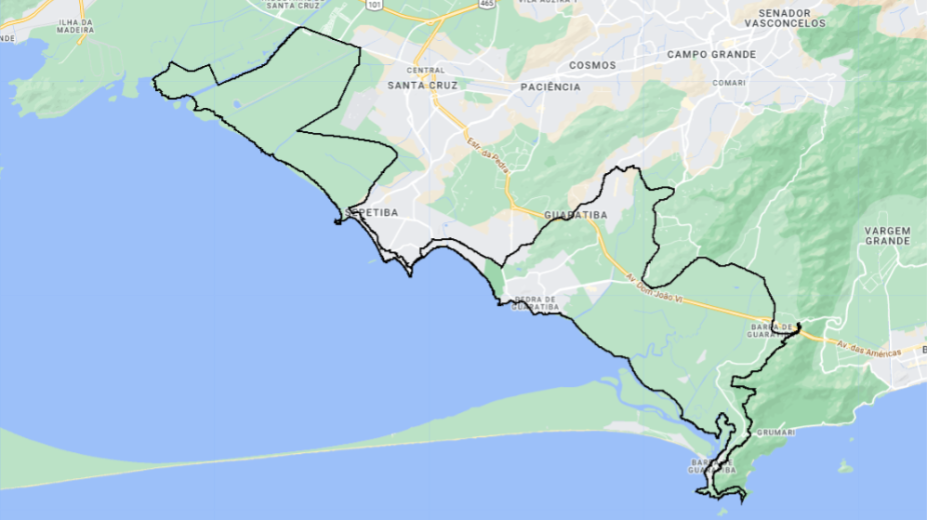
\includegraphics[width=0.7\textwidth]{Figures/chap4/apa_sepetiba.png}
\caption[APA da Orla da Baía de Sepetiba]{Tentative boundaries of the proposed planned \ac{apa} da Orla da Baía de Sepetiba.}
\label{fig:apa_sepetiba}
\end{figure}


Beyond the work presented in this chapter, analysis and reports have been commissioned on a variety of specific topics in the Guaratiba area, from reforming the educational system \cite{pizzolatoLOCALIZACAOESCOLASPUBLICAS2013} to the installation of green infrastructure \cite{herzogGuaratibaVerdeSubsidios2009} to means of protecting both the marine life and the artisan fishers of the area \cite{lopesTerritorialidadesEmConflitos2013}. A comparison of such reports does bring to light certain key themes, some high priority action items that the city or region could pursue. These include:

\begin{itemize}[itemsep=0pt,parsep=0pt]
	\item{Create a proper sewage and water treatment system. This would improve the health of both the people and the environment and could make use of the natural drainage geography of the Guaratiba basin.}
	\item{Create a tiered licensing authority to permit certain low-impact artisanal activities in protected areas, while maintaining restrictions on higher impact activities. Once again, this helps the environment while also providing some degree of economic security for the historical residents.}
	\item{Strengthen environmental protections in forest-adjacent areas, such as construction limits in the Barra de Guaratiba neighborhood. This would prevent indirect pressures on the mangroves and slow both real estate speculation and commercial development, thereby preventing existing residents from being forced out.}
\end{itemize}

These items are merely specific, ad hoc solutions to a broader, meta-problem. Despite the overabundance of municipal, state, and federal government agencies operating in the area, there is no cohesive governance of the environment, the local residents (largely informal settlers), and their interactions. Without this, it is unlikely the any of these ideas will be properly implemented and broader economic forces healthily channeled. There are multiple options for such a governance structure. It could be a top-down entity, one that manages the entire drainage basin, such as the Tennessee Valley Authority or any of its numerous imitators around the world. It could also be a bottoms-up, mass participatory effort by the various communities of the area. Either way, such an entity would be able to not only implement these high priority items, but a host of others as well, such as managing the currently ad hoc diverting of the numerous regional waterways by government agencies, companies, and individuals, much to the detriment of the people and mangroves living downstream.

Unfortunately, neither option seems particularly likely at this time. As mentioned earlier, the city, state, and federal governments are either focused on other things or actively inamicable to such an effort. The residents, for the most part, seem to have little tradition of collective action outside of their profession (such as the protests of the steel mill by fishers) or their immediate neighborhood (such as Araçatiba-based advocacy for formal recognition). 

The author does not have the expertise or the experience with the region necessary to either recommend a specific course of action or predict the likely outcome these ongoing changes in Guaratiba. What can be said with certainty is that there is a real need for awareness raising in the area.

\subsection{\hlc[cyan]{Methodological Limitations and Potential Improvements}} \label{sec:rio-limitations}

This project was by no means a flawless execution of the \ac{evdt} Framework, nor does it resolve all the questions the stakeholders have. This section will review such limitations and consider opportunities for future projects (\ac{evdt} or otherwise) in the area. 

\subsubsection{\hlc[cyan]{Environment}}

The assessment of mangrove extent, health, height, and \ac{agb} involved various simplifications and assumptions, some of which were briefly noted in Sections \ref{sec:rio-evdt-e-method} and \ref{sec:rio-evdt-e-result}. 

First, as noted in Table \ref{tab:rio-environment-sources}, the \ac{gmw}v2 extent map was used for as a point of comparison and to assist selection of training data. Since this work was originally performed, \ac{gmw} has since released a v3 that includes annual extent maps for 2017-2020 and fixes various errors in previous version \cite{buntingGlobalMangroveExtent2022}.If this analysis were to be preformed again, it should be updated to the most current version of the \ac{gmw} dataset.

Second, the Rio de Janeiro area contains three different species of mangroves (\textit{Avicennia schaueriana}, \textit{Laguncularia racemosa}, \textit{Rhizophora mangle}), each of which have somewhat different spectral reflectance properties. This can introduce additional errors into identification and health.

As mentioned in Section \ref{sec:rio-evdt-e-method}, \ac{ndvi} is not a perfect measure of mangrove health in a multi-species ecosystem, but it is broadly accurate. With greater number of bands (more than 10) in the visual spectrum, it is sometimes possible to differentiate vegetation species in some cases, but existing free hyperspectral platforms have some combination of poor spatial resolution and insufficient coverage, making them inadequate for this application \cite{mousivandGlobalSensitivityAnalysis2014}. The upcoming launch of the Planet Tanager constellation may alter this situation \cite{planetlabspbcPlanetAnnouncesNew2022}. In the future, such hyperspectral imagery may allow for distinguishing one species of mangrove overtaking another from changes in mangrove health. 

Next, the analyses in this case study relied upon Simard et al.'s \ac{srtm}-based height estimation from a particular year \cite{simardMangroveCanopyHeight2019}. It is possible to gather height information on additional years or at improved spatial resolution using aerial photogrammetry or \ac{lidar} \cite{olagokeIndividualMangroveTree2015}. Rio de Janeiro has recently conducted such a survey of the entire municipality, though the data was not available in time for this work. Future work though could make use such data, providing at least one additional point in time. Historical height data can also be estimated using space-based \ac{lidar} and \ac{sar} data \cite{lagomasinoComparisonMangroveCanopy2016}, though this method lacks the spatial resolution of aerial methods.

Finally, in Section \ref{sec:rio-evdt-e-result} I noted substantial differences in this estimate of \ac{agb} (based on one of Simard et al.'s allometric models) to those of Estrada et al. \cite{estradaEconomicEvaluationCarbon2015}. Hyperspectral-based species differentiation and higher resolution height measurements could enable a refinement of the allometric models used, improving \ac{agb} estimates. 

\subsubsection{\hlc[cyan]{Vulnerability}}

Despite the limitations in the environmental data discussed just above, its spatial and temporal resolutions were actually quite fine compared to the bulk of the socioeconomic data used in this study. Most employment and population data was available only on a decennial basis and much of it was at the neighborhood or \ac{ra} level, rather than the 30m of much of the satellite data. 

There are multiple potential ways to overcome this. One method is to get access to finer grain socioeconomic data collected by \ac{ibge}, Brazil's national statistical agency. \ac{ibge} does in fact have a process for this though it requires pre-approval of the analysis method and the data to be used, for the analysis to take place in-person at a particular \ac{ibge} office, and that only anonymized, aggregate statistics are removed from the site \cite{institutobrasileirodegeografiaeestatisticaPedidosComoFazer2014}. Conveniently enough, this facility is located in the city of Rio de Janeiro. Several collaborators and I were considering just such an option, including sketching out what kind of analysis would be most useful to support the \ac{dss}, when the onset of the pandemic resulted in the closure of such nonessential government facilities and sent me back to the US. 

Another method would be to simply ask, that is to conduct household surveys or surveys of local tourism and aquaculture businesses. This could have not only provided the useful socioeconomic data, but also could have furnished useful information on how local stakeholders valued ecosystem services and the local mangroves. Such surveys could have involved direct reporting or more sophisticated choice experiments. I consulted with Suhyun Jung, an ecosystem services economist with experience with such approaches \cite{jungBrazilNationalEnvironmental2017, jungPartnershipsPreventDeforestation2018, jungEvidenceWealthImprovingEffects2019a}, about doing just this. This resulted in an ongoing collaboration, sadly beyond the scope of this thesis, to better understand and quantify the dynamics linking mangrove health and conservation policies with local socioeconomic impact. In this study historical data and potentially household surveys will be used in conjunction with the mangrove health history to estimate the "Carbon and Raw Material Impact" and "Local Socioeconomic Impact of Mangrove Loss," as shown in Figure \ref{fig:method}. This represents a refinement of the \ac{evdt} analyses performed in this chapter. Once these historical dynamics are better understood, we can progress to predictive simulation of vulnerability.

\begin{figure}[!htb] 
\centering
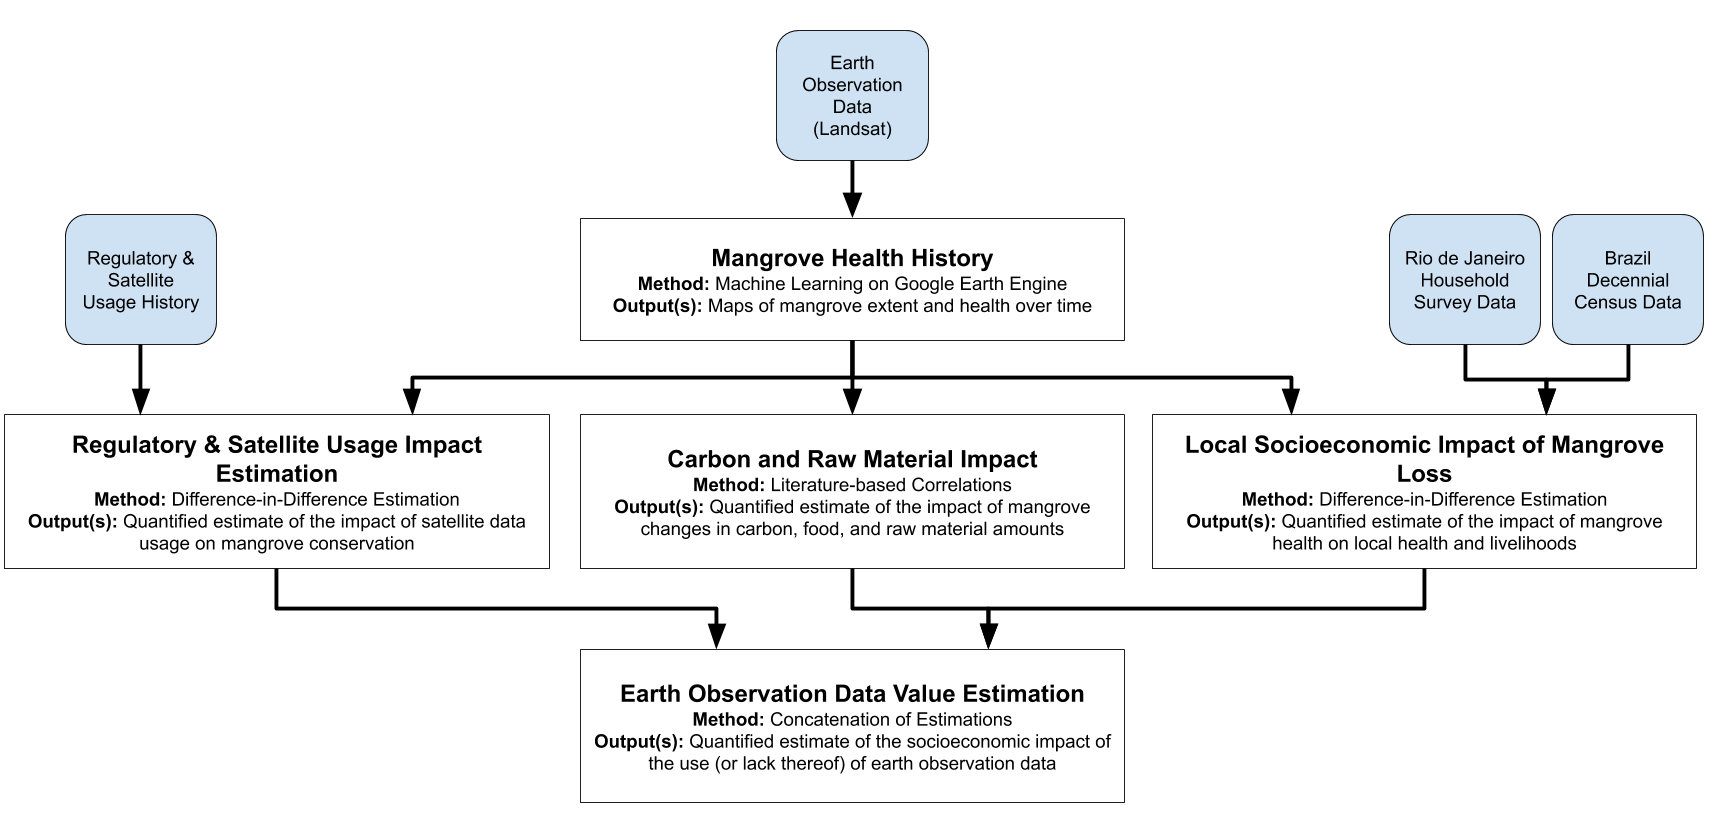
\includegraphics[width=0.9\textwidth]{Figures/chap4/Method_Flowchart.png}
\caption{Flowchart indicated various ways of estimating causal impact of one EVDT component on another}
\label{fig:method}
\end{figure}

A more novel method would have been to apply a similar kind of remote observation analysis used to assess the mangroves to assess the socioeconomic state of the region. Salas et al. have recently demonstrated the viability of using fine-grained census data in combination with Landsat imagery to train a deep learning model to estimate various forms of socioeconomic vulnerability in Mexico \cite{salasFineGrainedLargeScaleVulnerable2021}. Such a method could be used to generate annual assessments between decennial census data.

\subsubsection{\hlc[cyan]{Decision-Making}}

Only a rudimentary analysis of the relationship between environmentally protected areas and planning zones with mangrove health and extent was conducted in this chapter. The aforementioned collaboration with Jung (Figure \ref{fig:method}, could help expand this analysis. Further improvements could be obtained by examining when changes in policy occurred (such as the creation of a protected area) to see if a natural experiment could be constructed. This might help not only determine the directionality of the casual impact of such policies on the mangroves, but perhaps even to measure the magnitude. 

Other potential improvements could involve considering enforcement of the policy decisions. During each of my visits to the \ac{rbag}, I witnessed locals fishing among the mangroves, an activity that is nominally prohibited within the reserve. The number of informal settlements throughout Rio de Janeiro similarly suggest that planning zones are not always strictly adhered to. If enforcement of these policies has varied over time, particularly if such variation has gone unrecorded, it could muddy the waters when seeking to determine what impact different policies have on the mangroves.

On the other hand, studying such variations in enforcement could provide insight onto which aspects of protected areas and planning zones (each of which are essentially a bundle of many different regulations) are actually most relevant for protected mangroves. It is entirely possible that small-scale, artisanal fishing and timber harvesting (important ecosystem services) within the \ac{rbag} would not harm the mangroves or their ecosystem. If this is the case, such sustainable use of the forests could be officially licensed, providing additional legal and economic security to the local communities. Future work could examine this very question.

In addition to conservation, there is the potential for replanting and restoration of mangroves. Numerous replanting and restoration projects have taken place in the Rio de Janeiro area in recent years, both in dedicated conservation areas \cite{granadoAssessingGeneticDiversity2018} and in more urban and peri-urban areas \cite{rioprefeituraEnvironmentalRecoveryRodrigo2019, soaresEstruturaVegetalGrau1999}. There is evidence that such replanting projects can cause the soil to rapidly regain carbon storage and sequestration capacity \cite{jimenezRecoverySoilProcesses2022}.

Siting of these restoration areas ideally depends both on the environmental viability of a potential site and its likely ecosystem service impacts. As discussed in Section \ref{sec:rio-saf-objectives-result}, some government initiatives have replaced mangroves lost to development with replanting projects elsewhere in the region. The local fishing community, who more directly rely upon the local non-carbon ecosystem services, would prefer to have more control over where such replanting efforts occur. There is potential for an \ac{evdt} project aimed specifically at balancing such stakeholder concerns when siting restoration areas.


\subsubsection{\hlc[cyan]{Technology}}

The technology component in this case study was the most underdeveloped of the four \ac{evdt} components. Two potential expansions are readily apparent. The first would be a more detailed study of the historical relationships between the use of \ac{eo} data and environmental or socioeconomic phenomena. Does increased use of such data result in better outcomes? The project with Jung, shown earlier in Figure \ref{fig:method}, would attempt to partially address this via its ``Earth Observation Data Value Estimation." This would be accomplished both by studying variations in the use of \ac{eo} data by Rio de Janeiro over time and by comparison to other nearby municipalities that either do or do not make use of such data. 

Another method would be to integrate choice of sensing technologies into the \ac{dss}, turning it into a kind of urban planning \ac{osse}. This was considered in early phases of this project. The concept was that, when the \ac{dss} was initialized, the user would be presented with a screen asking them to select what datasets they wished to rely upon. Figure \ref{fig:data_source_selection_panel} shows a mockup of such a screen from when this was being considered. The \ac{dss} would then adjust the spatial and temporal resolution of both the real world data presented and the generated scenarios. By comparing their ability to make informed decisions under each of these different data source situations, the user could start to assess how valuable each sensing technology was. 

Either of these two methods could help inform stakeholders as to the extent to which they should prioritize integrating \ac{eo} into their decision-making processes, either in terms of money or capacity building. For instance, they could determine whether freely available Landsat imagery was sufficient for their needs or whether commissioned high resolution Worldview surveys were necessary. 

Ultimately, however, neither of these two methods were pursued during this case study itself. This was essentially because making such \ac{eo} data acquisition decisions was only relevant to a subset of stakeholders (primarily \ac{ipp} and \ac{smac}, secondarily to \ac{smu}) and even to them it was considered a lower priority than using currently available data more effectively. Both approaches remain intriguing possibilities for future work, however.


\begin{figure}[!htb] 
\centering
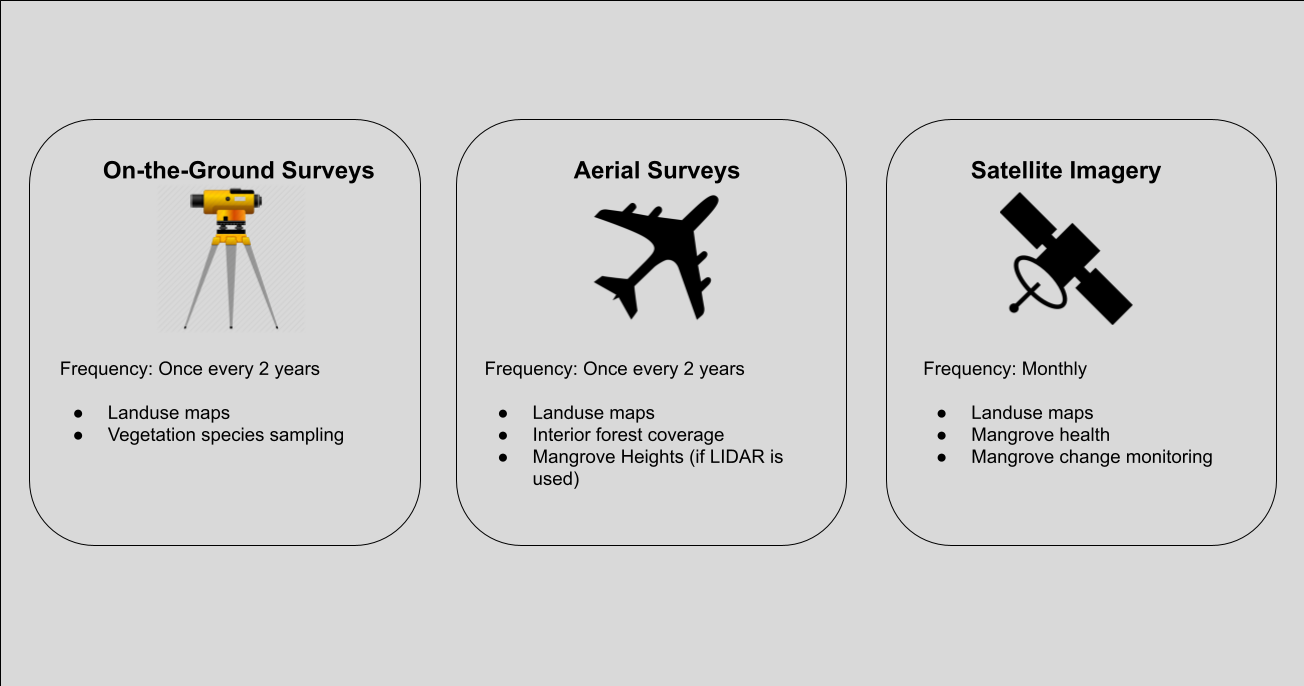
\includegraphics[width=0.9\textwidth]{Figures/chap4/data_source_selection_panel.png}
\caption[Mockup of Rio DSS Data Source Selection]{Mockup of a proposed data source selection panel in the \ac{dss}.}
\label{fig:data_source_selection_panel}
\end{figure}
	

\subsubsection{\hlc[cyan]{Stakeholder Collaboration and Engagement}} \label{sec:rio-discuss-stakeholder}

As stated in Section \ref{sec:rio-collab}, stakeholder participation and collaboration was less than desired or planned for in multiple ways, reducing the impact of this project. While this is partially attributable to the pandemic, other actions could have been taken to minimize such impacts. I could have switched to conducting remote interviews over platforms such as Zoom and could have reconfigured the planned user study workshops to function in a virtual or hybrid environment. It is unlikely that these would have been able to reach all of the involved stakeholders, as both internet access and familiarity with computers vary across the city, but I would have been able to maintain a higher level of stakeholder participation.

There was also a missed opportunity to engage at least some of the stakeholders in direct coding of the \ac{dss} or \ac{evdt} analysis. Out of desire to increase accessibility to a variety of stakeholders, I placed an emphasis on the \ac{dss} being written from the ground up in Python as a free and open-source project. Similarly, I conducted much of the analysis using the free (though not entirely open-source) \ac{gee}. This failed to recognize that the stakeholders most likely to directly participate in the coding and analysis (\ac{ipp} and ESPAÇO) were not familiar with either Python or \ac{gee}. Instead they were familiar with and active users of ESRI's ArcGIS products (which are notably neither free nor open-source). It may have been more worthwhile to focus efforts on software and processes that could be more easily integrated into existing processes. That said, such a course of action would raise the potential for merely confirming existing processes (particularly governmental processes) at the expense of less digitally enfranchised stakeholders. 

Additionally this case study did not contact or seek to involve certain stakeholders not in regular communication with the network shown in Figure \ref{fig:rio_stakemap}. Among these are the \ac{inpe}, Brazil's space agency. I had originally planned on contacting them with regards to this project and including them as a secondary stakeholder, including to go as far as to sketch out a potential user experience \ref{fig:concept_flow}. Ultimately it became clear that \ac{inpe} is primarily focused on the Amazon rainforest and does not generally involve itself in municipal affairs. The primary envisioned role of \ac{inpe} was in selecting or even designing new \ac{eo} platforms as part of the Technology component, along the lines of the \ac{cbers} program. When this component was de-prioritized (as discussed in the previous section, I was de-prioritized contacting \ac{inpe}. 

Another potential contacted stakeholder would be officials in the EU legislatures, regulatory bodies, or investors. During initial stakeholder outreach, a member of the Pedra de Guaratiba Fishers Association mentioned that a number of years ago, they sent a delegation to protest the expansion of the (EU-headquartered) steel mill before such bodies. Presenting the ecosystem services impact of such projects could be another use of the analysis here or a properly designed \ac{dss}. 

\subsubsection{\hlc[cyan]{Decision Support System}}

As stated in Section \ref{sec:rio-dss}, certain aspects of the \ac{dss} system remain undone and many others remain largely untested. Not all of the data and results presented in Section \ref{sec:rio-evdt-result} were integrated into the \ac{dss}. One of the most notable such items were the ecosystem services value estimations. Ideally these would have been presented both in total in the \textit{Exibição de Dados} and spatially on a per bairro basis (and/or the other units of analysis).

Another unimplemented feature is, beyond changing the category of protected areas or planning zones, the ability to alter their boundaries or define entirely new such areas. This would have been particularly relevant for using the \ac{dss} for defining the boundaries or policies of the new \ac{apa} da Orla da Baía de Sepetiba (discussed earlier in this section). In the fall of 2022, I discussed with individuals at \ac{ipp} and \ac{smac} the prospect of renewing this project with specifically this purpose in mind. Ultimately it was decided that the time scale for such endeavors would put it outside the conclusion of this doctoral program. That said, it remains a potential future \ac{evdt} project for another student or researcher. 

Another point worth noting is that there were significant drawbacks to having a desktop-based system rather than an online system. While there were reasons for this choice (see Section \ref{sec:rio-dss}), in retrospect it seems to have limited both the usability of the \ac{dss} and the ability to receive prompt feedback, particularly once the pandemic set it. Such issues were seen again in the Vida project (Chapter \ref{ch:vida}). Based on both of those experiences, I can state that hosting the \ac{dss} online is generally to be preferred and more recent \ac{evdt} projects informed by this experience, such as Jaffe's thesis work \cite{jaffeEnvironmentalEconomicSystems2022}, seem to have performed better.  

\subsection{\hlc[cyan]{Lessons Learned for the EVDT Framework}} \label{sec:rio-lessons-learned}

This case study was one of the first full implementation of the \ac{evdt} Framework, or at least its initial version of it, alongside Ovienmhada's water hyacinth project in Benin \cite{ovienmhadaInclusiveDesignEarth2021}. As such it, both its successes and shortcomings (many of which were noted above) directly informed revisions of the framework, leading to the version presented in Chapter \ref{ch:evdt}. It is worth detailing some of these specific lessons learned.


\textbf{The need for the two separate iterations of the \ac{saf}.} Earlier version of the \ac{evdt} Framework where not as strictly linear as Figure \ref{fig:evdt_framework}. Both the \ac{saf} and the \ac{evdt} components were viewed as spanning the entire project and not being particularly distinct, with only one iteration of the \ac{saf} explicitly called for. 

This led to ambiguity about whether the \ac{evdt} practitioner should be focusing the \ac{saf} process on the existing {sets} that the community is operating in or on the \ac{dss} that was to be developed. Lombardo et al., working on coastal flooding in Indonesia, situate the Space Enabled researchers as the primary stakeholder, the \ac{evdt} components as the System Form, and the \ac{dss} as the output of the process \cite{lombardoEnvironmentVulnerabilityDecisionTechnologyFrameworkDecision2022}.   Jaffe meanwhile situated herself as a secondary stakeholder (advising the primary stakeholders involved in cranberry farming and restoration in Massachusetts) but still focused the \ac{saf} process on defining requirements for the \ac{dss} \cite{jaffeEnvironmentalEconomicSystems2022}. Ovienmhada et al. took the time to define the forms and functions of the existing water hyacinth harvesting \ac{sets} in Benin prior to embarking on the design of the \ac{dss} \cite{ovienmhadaInclusiveDesignEarth2021}. Even this case study did not clearly separate the two (note that there is only one \ac{saf} section in this chapter). 

Through this case study and through comparison with the above cited peers of mine, we realized that it is important to first use the \ac{saf} to define and provide information on the existing \ac{sets} that stakeholders live in, then frame that \ac{sets} using the \ac{evdt} components, and only then embark on the design of a \ac{dss} using the \ac{saf}. This helps to avoid putting the cart before the horse and forcing a particular pre-conceived solution architecture upon the stakeholders. 

\textbf{The importance of Local Context Experts.} While stakeholder participation and collaboration was key to the \ac{evdt} framework in even its earliest versions, the importance of Local Context Experts as discussed in Section \ref{sec:intended} was not fully appreciated. 

In particular the importance of having firm connections to multiple stakeholders can be critical to properly involving as many stakeholders as possible. In this project, \ac{ipp} is situated as a reasonably neutral data provider and occasional mediator between other, sometimes rivalrous government agencies. Having introductions furnished by \ac{ipp} enabled for serious and engaged discussions with both \ac{smac} and \ac{smu}, for instance, where otherwise I may have been typecast as aligned with one or the other and dismissed accordingly.  

Similarly working with ESPAÇO, a local university research group with close ties to the Guaratiba area and its communities, enabled interactions with stakeholders that would have been difficult if not impossible if arranged by government officials. Even so, I was not able to contact some more explicitly activism-oriented groups, as noted in Table \ref{tab:rio-contacts}.

Sometimes, however, such alignment with certain stakeholders is desirable even if it runs the risk of alienating others, but such a decision should be consciously and explicitly made. Ovienmhada et al., for example, working on environmental justice in carceral landscapes of the US, intentionally positioned the project as a social justice endeavor that was aligned with prison abolition activists \cite{ovienmhadaEnvironmentVulnerabilityDecisionTechnologyModelingFramework2021}. 

\textbf{The importance of appropriately scoping an \ac{evdt} project.} Involving as many stakeholders as possible and taking the multidisciplinary approach called for by the \ac{evdt} Framework can quickly cause a project to balloon out of the realm of feasibility. As noted in Section \ref{sec:rio-limitations}, there were innumerable other avenues that this project could have taken (and could still take in the future!). 

This problem was exacerbated in this case by this being the initial trial of a new framework, being run by a new research group. As a result, there was not an abundance of reference materials and code, nor was there experience and institutional knowledge. Hopefully future projects, able to learn and build upon the experience of this and the other first generation of \ac{evdt} projects, will be able to more quickly identify a path and implement it.


\section{\hlc[cyan]{Conclusion}}

This chapter presented one of the first implementations of the \ac{evdt} Framework: supporting decision-making regarding the mangroves of Sepetiba Bay and the communities that live near them. I detailed the history of the Guaratiba \acl{sets} and its complicated network of stakeholders before presenting a series of analyses on mangrove health, carbon sequestration, ecosystem services, and sensitivity to government policy decisions. These were used to construct a prototype \ac{dss} for setting environmental protected areas and planning zones. 

In doing so, this case study not only supported stakeholders' decision-making, but it also provided a demonstrated of the \ac{evdt} Framework, thereby helping to respond to Research Question 2: ``What are the sustainability benefits of collaborative development of \acp{dss} using the \acf{evdt} Modeling Framework in complex \acf{sets}?"

This implementation was not without its flaws and this experience informed refinements of the \ac{evdt} Framework. The following chapter will repeat this process for another case study, the Vida \ac{dss} International Network. This will be followed by Chapter \ref{ch:discussion} in which both case studies and the framework itself will be reviewed and future improvements and opportunities will be noted.




